\clearpage
\section{Method evaluation}
\label{sec:methodEvaluationChapter1}
In this section we perform a full evaluation of the presented methods, under different parametrizations, on several shift-estimation tasks. For experimentation, all experiments were done using a high-resolution satellite image of the city of Cannes \ref{fig:CannesChapter1}. In a simulated environment, $I_1$ was generated by taking a $50 \times 50$ subimage from a random location, while $I_2$ was obtained by shifting the high-resolution image in the Fourier domain using Eq.~\eqref{eq:FourierShiftTheoremComplete} followed by taking a subimage with the same size and from the same location. All shift estimation errors were computed as the root mean squared error (RMSE) and are in pixels. This implies that if $\bv$ and $\hat{\bv}$ are the real shift and the estimated shift, then the error obtained is
\begin{equation}
	E(\hat{\bv}) = \sqrt{\frac{(v_x - \hat{v}_x)^2 + (v_y - \hat{v}_y)^2}{2}}.
\end{equation}
Results presented in this evaluation are, in every case, obtained by averaging 100 realizations.

\begin{figure}[htpb]
\centering
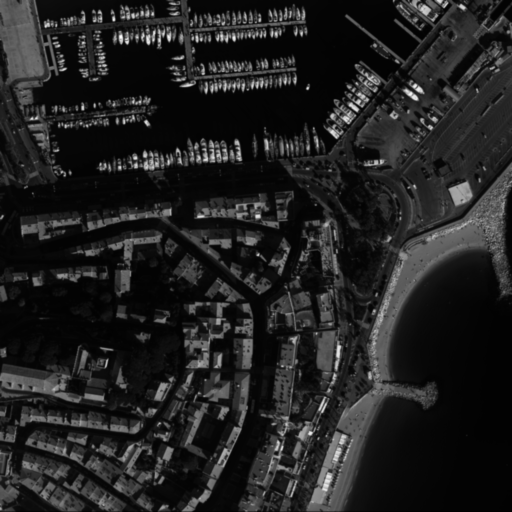
\includegraphics[width=.5\textwidth]{img/Cannes}
\caption{Input image used for simulation.}
\label{fig:CannesChapter1}
\end{figure}

Apart from the most important shift-estimation methods introduced in the previous section, five more approaches coming from the remote sensing community were also evaluated. Three of these methods (SDF, ADF and ADF2 \cite{lofdahl2010evaluation}) are loosely based on correlating both images followed by fitting a conic section in the 2D neighbourhood around the peak, while ACC \cite{Sidick2007} and APC \cite{Sidick2011} are two iterative methods, the former being based on the method of Stone \cite{Stone_2001} while the latter is based on a periodic correlation technique.

Due to the extensive amount of evaluated methods and variants, we defined a nomenclature to refer to each of them. In Table \ref{tab:nomenclatureForShiftEstimation} we observe all evaluated methods together with their parameters. For every method, parameter \itParam \ refers to the amount of iterations ($\itParam \in [1,2,3,4]$ in our experiments), \grParam \ to a gradient estimation method presented in section \ref{sec:gradEstimationGBSE} (Table \ref{tab:gradEstimationGBSE}), \intParam  \ to an interpolation method presented in section \ref{sec:interpolationChapter1}  (Table \ref{tab:interpolationMethodsGBSE}), \spParam \ to the support size, \emph{\textbf{up}} \  to the upsampling factor, \winParam \ to the apodization window used (Table \ref{tab:ApodizationWindows}) and \dParam \ to the dimensionality of the solution ($\dParam \in [1,2]$). 

For the multiscale GBSE method (MS), we first put the amount scales followed by a coma. Then we specify its configuration by putting for each scale the amount of iterations \itParam \ followed by the interpolation method \intParam \ used in each scale from the finest to the coarsest scale. For example, MS-3,321-IdssGh represents three scales, with a single iteration and spline interpolation on the coarsest scale, followed by two iterations and spline interpolation in the intermediate scale, and finally doing three iterations and DFT interpolation with symmetrization in the original scale, and where the image gradients are always computed using the hypomode.
\begin{table}[htpb]
\centering
\footnotesize
\begin{tabular}{c|l|l|c}
Code & Parameters & Method & Reference\\ \hline
LS & LS-\itParam-I\intParam-G\grParam & Least Squares GBSE & Alg.~\ref{algo:iterativeGBSEChapterShift}\\
TLS & TLS-\itParam-I\intParam-G\grParam & Total Least Squares GBSE & Eq.~\eqref{eq:tlsSolution} \\
CLS & CLS-\itParam-I\intParam-G\grParam & Corrected Least Squares GBSE & Eq.~\eqref{eq:CLS} \\
ULS & ULS-G\grParam & Bidirectional bias correction GBSE & \cite{pham2008} \\ \hline
MS & MS-\scParam,\itParam-I\intParam G\grParam & Multiscale GBSE & Alg.~\ref{algo:MSChapterShift} \\ \hline
INT & INT-\spParam & Interpolation method & Sec.~\ref{sec:interpolationMethod2013} \\ \hline
PC-GUIZAR & PC-GUIZAR-\emph{\textbf{up}} & Zero-fitting the cross-power spectrum  & \cite{Guizar-Sicairos08}\\
PCSTONE & PCSTONE-W\winParam & Robust plane fitting on the phase difference matrix & \cite{Stone_2001}\\
PC-QUADFIT & PC-QUADFIT-W\winParam & Quadratic fitting on the phase correlation surface & \cite{Abdou1998} \\
PC-GAUSSFIT & PC-GAUSSFIT-W\winParam & Gaussian fitting on the phase correlation surface & \cite{Abdou1998} \\
PCFOO & PCFOO-W\winParam & Max. of sinc approx. to phase correlation surface & \cite{Foroosh2002} \\
PC-SINC & PC-SINC-W\winParam & Sinc fitting on the phase correlation surface & \cite{Argyriou2006} \\
PC-ESINC & PC-ESINC-W\winParam & E-Sinc fitting on the phase correlation surface & \cite{Argyriou2006} \\
PC-LCM & PC-LCM-\dParam D\spParam & \dParam-dimensional local center of mass of the PCS  & \cite{Alba_2015} \\
PC-REN2010 & PC-REN2010-W\winParam & Difference between both side-peaks of the PCS & \cite{Ren_2010} \\ \hline
SS-HOGE & SS-HOGE-W\winParam & Subspace method by Rank-1 approximation & \cite{Hoge_2003} \\
SS-ROBINSON & SS-ROBINSON-W\winParam & Projection-based subspace phase correlation & \cite{Robinson_2001} \\
SS-REN2014 & SS-REN2014-W\winParam & Projection-based subspace gradient correlation & \cite{Ren_2014} \\ \hline
GC04 & GC04-G\grParam & Gradient Correlation & \cite{Argyriou2004} \\
GC11 & GC11-G\grParam & Kernelized Gradient Correlation & \cite{Tzimiropoulos2011}\\ 
NGC04 & NGC04-G\grParam & Normalized Gradient Correlation & \cite{Argyriou2004} \\
NGC11 & NGC11-G\grParam & Kernelized Normalized Gradient Correlation & \cite{Tzimiropoulos2011}\\ \hline
SDF & SDF-2QI & Sum of squared differences  & \cite{lofdahl2010evaluation}\\
ADF & ADF-2QI & Sum of absolute differences differences & \cite{lofdahl2010evaluation}\\
ADF2 & ADF2-2QI & Sum of squared absolute differences differences & \cite{lofdahl2010evaluation}\\
ACC & ACC-\itParam It & Adaptive Cross-Correlation & \cite{Sidick2007}\\
APC & APC-\itParam It & Adaptive Periodic-Correlation & \cite{Sidick2011}\\ \hline
\end{tabular}
\caption{Method references for this evaluation section.}
\label{tab:nomenclatureForShiftEstimation}
\end{table}

\begin{table}[htpb]
\centering
\scriptsize
\begin{minipage}[t]{.38\textwidth}
\vspace{0pt}
\begin{tabular}{c|l}
Code & Name\\ \hline
h & Hypomode \\
g0.3 & $3 \times 3$ Gaussian derivative $\sigma=0.3$\\
g0.6 & $5 \times 5$ Gaussian derivative $\sigma=0.6$\\
g1 & $7 \times 7$ Gaussian derivative $\sigma=1$\\
sim3 & $3 \times 3$ Simoncelli derivative \\
sim5 & $5 \times 5$ Simoncelli derivative \\
sim7 & $7 \times 7$ Simoncelli derivative \\
fa3 & $3 \times 3$ Farid derivative \\
fa5 & $5 \times 5$ Farid derivative \\
fa7 & $7 \times 7$ Farid derivative \\
ch1 & 1st order Christmas derivative \\
ch2 & 2nd order Christmas derivative \\
ch3 & 3rd order Christmas derivative \\ \hline	
\end{tabular}
\caption{\scriptsize{Evaluated gradient estimation method codes \grParam.}}	
\label{tab:gradEstimationGBSE}
\end{minipage}%
\begin{minipage}[t]{.25\textwidth}
\vspace{0pt}
\begin{tabular}{c|l}
Code & Name\\ \hline
nw & No Window\\
ex & Image zero-padding\\
bm & Blackman\\
bh & Blackman-Harris \\
bl & Bartlett \\
bw & barthann  \\
cw & Chebyshev\\
gw & Gaussian\\
hw & Hamming \\
tw & Tukey \\
ft & Flat-top\\ \hline	
\end{tabular}
\caption{\scriptsize{Window codes \winParam \ used for apodization.}}	
\label{tab:ApodizationWindows}
\end{minipage}\hspace{0.7em}
\begin{minipage}[t]{.35\textwidth}
\vspace{0pt}
\begin{tabular}{c|l}
Code & Name\\ \hline
l & Bilinear interpolation\\
c & Bicubic interpolation\\
s & 3rd order spline interpolation\\
f & FFT interpolation\\
d & FFT with symmetrization int.\\ \hline	
\end{tabular}
\caption{\scriptsize{Evaluated interpolation method codes \intParam.}}
\label{tab:interpolationMethodsGBSE}
\end{minipage}%
\end{table}

As mentioned in section \ref{sec:introShiftEstimation}, when evaluating the methods in the presence of noise, we assumed white Gaussian noise uncorrelated with the signal. Simulating Ren \emph{et al.} \cite{Ren_2010}, we discretized the noise into five distinct levels (five different values for the noise standard deviation $\sigma_N$), shown in Table \ref{tab:noiseLevels}, and used this categorization to evaluate the methods.

\begin{table}[ht!]
\centering
\begin{tabular}{|c|c|c|c|c|c|} 
	\hline
	Level & 1 & 2 & 3 & 4 & 5\\ \hline
	$\sigma_N$ & 0.000 & 0.005 & 0.015 & 0.025 & 0.055\\ \hline
\end{tabular}
\caption{Std. dev. of white Gaussian noise for each noise level injected to the simulated images.}
\label{tab:noiseLevels}
\end{table}

In the same manner, all evaluated displacements were grouped into four categories. The reason behind this distinction is that some methods are more suited than others for each designated category. The ranges for each shift magnitude level are as shown in Table \ref{tab:shiftMagnitudeCategories}. In the first category, extremely small sub-pixel shifts were considered, as they could exist in several applications. We also include as a fourth category, magnitudes larger than 1.1 pixels. By design, all non-multiscale GBSE methods as well as the phase correlation method from Stone \cite{Stone_2001} fail under this category. Due to this reason, although being shown for completeness, this shift magnitude is excluded from the general averages on every table.

\begin{table}[htpb]
\centering
\begin{tabular}{|c|c|c|c|c|} 
	\hline
	Level & 1 & 2 & 3 & 4 \\ \hline
	Range & $\norm{\bv} \leq 0.1$ & $0.1 < \norm{\bv} \leq 0.5$ & $0.5 < \norm{\bv} \leq 1.1$ & $\norm{\bv} > 1.1$ \\ \hline
\end{tabular}
\caption{Shift magnitude ($\norm{\bv}$) ranges for each evaluated category.}
\label{tab:shiftMagnitudeCategories}
\end{table}

%To verify the performance of each method, the CRLB is calculated for every estimation, and a threshold of 0.04 determines if a shift estimation is preconsidered valid or not. Hence, results are divided into two groups: results including all estimations and results only including valid configurations. Tables \ref{tab:1it}, \ref{tab:2itL}, \ref{tab:2itC}, \ref{tab:3itL}, \ref{tab:3itC}, \ref{tab:3itS}, \ref{tab:4itS} and \ref{tab:ULS} shows the results for every evaluated method averaging over all evaluated noise levels and simulated shifts.

We begin our evaluation by studying the impact of gradient estimation methods on GBSE approaches.

\subsection{Influence of gradient estimation on GBSE methods}
Since GBSE methods are gradient-based, their performance obviously depends on the method used to estimate the image gradient. To this end, we evaluated several gradient estimation methods using the original least-squares approach as explained in section \ref{sec:gradEstimationGBSE}.  Emulating Ren \emph{et al.} \cite{Ren_2010}, we used all possible shifts obtained by taking two values from $[-0.875, -0.75, -0.5, -0.25, -0.125, -0.07, -0.02, 0, 0.03, 0.125, 0.25, 0.5, 0.75, 0.875]$. In total, this represented 196 shifts, from which for each experiment, a random sub	image was obtained and shifted in the frequency domain using the Fourier shift theorem. The average error obtained for all 196 shifts is shown in Fig.~\ref{fig:gradEvaluation} as the noise increases (left) or by varying shift magnitude (right) , using the five noise levels shown in Table \ref{tab:noiseLevels} and the four shift magnitudes of Table \ref{tab:shiftMagnitudeCategories}. 

Several conclusions are drawn following the preceding experiment. 
\begin{itemize}
	\item First, the most accurate gradient estimation method for GBSE proved to be the method of Farid \cite{farid2004differentiation}, followed by the approach of Simoncelli \cite{Simoncelli_1994}. 
	\item Second, the kernel support size should be set larger $(7 \times 7)$ under higher noise scenarios, and shorter ($3 \times 3$) when the SNR is high. 
	\item Third, using $\sigma=0.6$ for the Gaussian kernel always obtained the best results, however the performance using $\sigma=1$ seems less affected by higher noise situations, and should be considered in those cases. A more in-depth study on Gaussian gradient estimation performance for GBSE methods is given in the following section. 
	\item Finally, even though computationally cheap, the hypomode gradient estimation should be avoided when shift estimation is done on all possible shift magnitudes between the [-1,1] interval. Nevertheless, under low shift magnitudes and high noise, the hypomode becomes the most accurate method, as seen in Table \ref{tab:gradientEvaluationChapter1}, where the top 10 gradient estimation methods are shown depending on both the shift magnitude and the noise.
\end{itemize}

\begin{figure}[htpb]
\centering
\begin{subfigure}{.5\textwidth}
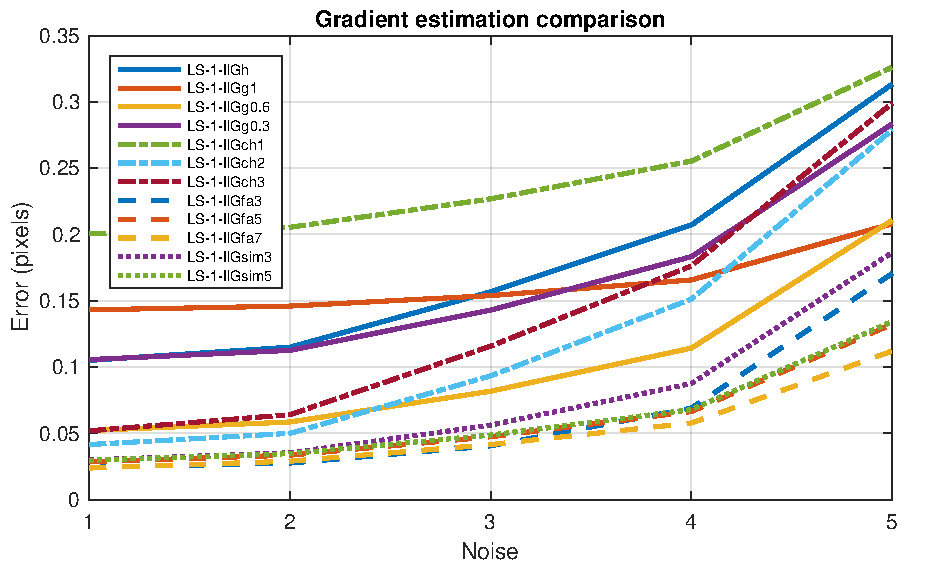
\includegraphics[width=\textwidth]{img/gradientEvaluation}
\end{subfigure}%
\begin{subfigure}{.5\textwidth}
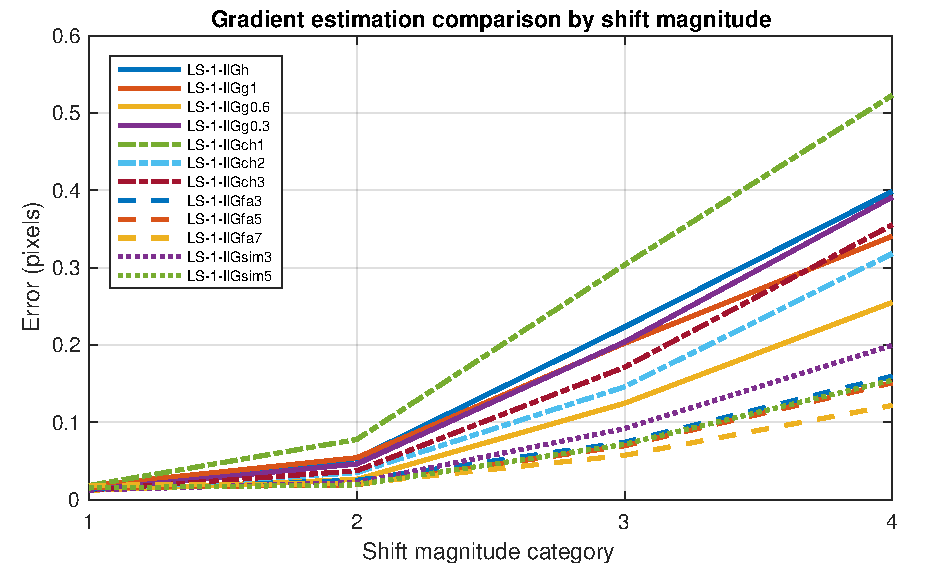
\includegraphics[width=\textwidth]{img/gradientEvaluationByShift}
\end{subfigure}
\caption{Comparison of accuracy obtained by using different gradient estimation methods on the GBSE algorithm. \textbf{Left}: By noise level. \textbf{Right}: By shift magnitude category.}
\label{fig:gradEvaluation}
\end{figure}

\begin{table}[htpb]
\centering
\scriptsize
\setlength{\tabcolsep}{1pt}
\renewcommand{\arraystretch}{1}
\begin{tabular}{|c|l|l|l|l|l|}\hline
& \multicolumn{1}{|c|}{$\norm{\bv} \leq 0.1$} & \multicolumn{1}{|c|}{$0.1 < \norm{\bv} \leq 0.5$} & \multicolumn{1}{|c|}{$0.5 < \norm{\bv} \leq 1.1$} & \multicolumn{1}{|c|}{$\norm{\bv} > 1.1$} & \multicolumn{1}{|c|}{Avg.}\\ \hline 
\begin{tabular}{c}$\sigma$\\$0.000$\end{tabular} & \begin{tabular}{l}0.0000\ LS-1-IlGfa7\\0.0001\ LS-1-IlGsim5\\0.0001\ LS-1-IlGfa5\\0.0007\ LS-1-IlGg0.6\\0.0015\ LS-1-IlGsim3\\0.0020\ LS-1-IlGch3\\0.0033\ LS-1-IlGch2\\0.0037\ LS-1-IlGfa3\\0.0045\ LS-1-IlGg0.3\\0.0048\ LS-1-IlGh\\\end{tabular} & 
\begin{tabular}{l}0.0010\ LS-1-IlGfa5\\0.0010\ LS-1-IlGfa7\\0.0012\ LS-1-IlGsim5\\0.0046\ LS-1-IlGg0.6\\0.0052\ LS-1-IlGsim3\\0.0067\ LS-1-IlGch3\\0.0128\ LS-1-IlGch2\\0.0150\ LS-1-IlGfa3\\0.0216\ LS-1-IlGg0.3\\0.0231\ LS-1-IlGh\\\end{tabular} & 
\begin{tabular}{l}0.0245\ LS-1-IlGfa3\\0.0290\ LS-1-IlGfa7\\0.0333\ LS-1-IlGsim3\\0.0347\ LS-1-IlGfa5\\0.0362\ LS-1-IlGsim5\\0.0420\ LS-1-IlGch2\\0.0583\ LS-1-IlGch3\\0.0641\ LS-1-IlGg0.6\\0.1305\ LS-1-IlGg0.3\\0.1315\ LS-1-IlGh\\\end{tabular} & 
\begin{tabular}{l}0.0733\ LS-1-IlGfa3\\0.0843\ LS-1-IlGfa7\\0.1025\ LS-1-IlGfa5\\0.1054\ LS-1-IlGsim5\\0.1163\ LS-1-IlGsim3\\0.1717\ LS-1-IlGg0.6\\0.1785\ LS-1-IlGch2\\0.2094\ LS-1-IlGch3\\0.2725\ LS-1-IlGh\\0.2952\ LS-1-IlGg0.3\\\end{tabular} & 
\begin{tabular}{l}0.0286\ LS-1-IlGfa7\\0.0291\ LS-1-IlGfa3\\0.0346\ LS-1-IlGfa5\\0.0357\ LS-1-IlGsim5\\0.0391\ LS-1-IlGsim3\\0.0592\ LS-1-IlGch2\\0.0603\ LS-1-IlGg0.6\\0.0691\ LS-1-IlGch3\\0.1079\ LS-1-IlGh\\0.1130\ LS-1-IlGg0.3\\\end{tabular}\\ \hline
\begin{tabular}{c}$\sigma$\\$0.005$\end{tabular} & \begin{tabular}{l}0.0039\ LS-1-IlGg0.6\\0.0041\ LS-1-IlGsim3\\0.0043\ LS-1-IlGch3\\0.0045\ LS-1-IlGsim5\\0.0045\ LS-1-IlGfa5\\0.0049\ LS-1-IlGch2\\0.0054\ LS-1-IlGfa7\\0.0055\ LS-1-IlGfa3\\0.0059\ LS-1-IlGg0.3\\0.0063\ LS-1-IlGh\\\end{tabular} & 
\begin{tabular}{l}0.0049\ LS-1-IlGfa5\\0.0050\ LS-1-IlGsim5\\0.0057\ LS-1-IlGfa7\\0.0061\ LS-1-IlGsim3\\0.0068\ LS-1-IlGch3\\0.0072\ LS-1-IlGg0.6\\0.0111\ LS-1-IlGch2\\0.0145\ LS-1-IlGfa3\\0.0238\ LS-1-IlGg0.3\\0.0264\ LS-1-IlGh\\\end{tabular} & 
\begin{tabular}{l}0.0260\ LS-1-IlGfa3\\0.0314\ LS-1-IlGfa7\\0.0374\ LS-1-IlGfa5\\0.0376\ LS-1-IlGsim3\\0.0390\ LS-1-IlGsim5\\0.0508\ LS-1-IlGch2\\0.0691\ LS-1-IlGg0.6\\0.0716\ LS-1-IlGch3\\0.1372\ LS-1-IlGg0.3\\0.1415\ LS-1-IlGh\\\end{tabular} & 
\begin{tabular}{l}0.0783\ LS-1-IlGfa3\\0.0867\ LS-1-IlGfa7\\0.1051\ LS-1-IlGfa5\\0.1080\ LS-1-IlGsim5\\0.1216\ LS-1-IlGsim3\\0.1774\ LS-1-IlGg0.6\\0.1923\ LS-1-IlGch2\\0.2267\ LS-1-IlGch3\\0.2863\ LS-1-IlGh\\0.3025\ LS-1-IlGg0.3\\\end{tabular} & 
\begin{tabular}{l}0.0311\ LS-1-IlGfa3\\0.0323\ LS-1-IlGfa7\\0.0380\ LS-1-IlGfa5\\0.0391\ LS-1-IlGsim5\\0.0423\ LS-1-IlGsim3\\0.0644\ LS-1-IlGg0.6\\0.0648\ LS-1-IlGch2\\0.0774\ LS-1-IlGch3\\0.1151\ LS-1-IlGh\\0.1173\ LS-1-IlGg0.3\\\end{tabular}\\ \hline
\begin{tabular}{c}$\sigma$\\$0.015$\end{tabular} & \begin{tabular}{l}0.0105\ LS-1-IlGch2\\0.0108\ LS-1-IlGch3\\0.0109\ LS-1-IlGg0.6\\0.0110\ LS-1-IlGsim3\\0.0110\ LS-1-IlGg0.3\\0.0118\ LS-1-IlGh\\0.0119\ LS-1-IlGfa3\\0.0132\ LS-1-IlGsim5\\0.0134\ LS-1-IlGfa5\\0.0154\ LS-1-IlGg1\\\end{tabular} & 
\begin{tabular}{l}0.0131\ LS-1-IlGsim3\\0.0142\ LS-1-IlGfa5\\0.0143\ LS-1-IlGsim5\\0.0156\ LS-1-IlGfa3\\0.0161\ LS-1-IlGfa7\\0.0176\ LS-1-IlGg0.6\\0.0178\ LS-1-IlGch2\\0.0232\ LS-1-IlGch3\\0.0362\ LS-1-IlGg0.3\\0.0432\ LS-1-IlGh\\\end{tabular} & 
\begin{tabular}{l}0.0400\ LS-1-IlGfa3\\0.0428\ LS-1-IlGfa7\\0.0510\ LS-1-IlGfa5\\0.0527\ LS-1-IlGsim5\\0.0622\ LS-1-IlGsim3\\0.0960\ LS-1-IlGg0.6\\0.1080\ LS-1-IlGch2\\0.1382\ LS-1-IlGch3\\0.1741\ LS-1-IlGg0.3\\0.1905\ LS-1-IlGg1\\\end{tabular} & 
\begin{tabular}{l}0.0993\ LS-1-IlGfa7\\0.1134\ LS-1-IlGfa3\\0.1224\ LS-1-IlGfa5\\0.1256\ LS-1-IlGsim5\\0.1563\ LS-1-IlGsim3\\0.2137\ LS-1-IlGg0.6\\0.2705\ LS-1-IlGch2\\0.3113\ LS-1-IlGch3\\0.3223\ LS-1-IlGg1\\0.3524\ LS-1-IlGg0.3\\\end{tabular} & 
\begin{tabular}{l}0.0435\ LS-1-IlGfa7\\0.0452\ LS-1-IlGfa3\\0.0502\ LS-1-IlGfa5\\0.0515\ LS-1-IlGsim5\\0.0606\ LS-1-IlGsim3\\0.0845\ LS-1-IlGg0.6\\0.1017\ LS-1-IlGch2\\0.1209\ LS-1-IlGch3\\0.1434\ LS-1-IlGg0.3\\0.1445\ LS-1-IlGg1\\\end{tabular}\\ \hline
\begin{tabular}{c}$\sigma$\\$0.025$\end{tabular} & \begin{tabular}{l}0.0161\ LS-1-IlGch2\\0.0162\ LS-1-IlGg0.3\\0.0165\ LS-1-IlGg0.6\\0.0166\ LS-1-IlGsim3\\0.0168\ LS-1-IlGch3\\0.0170\ LS-1-IlGh\\0.0175\ LS-1-IlGfa3\\0.0201\ LS-1-IlGch1\\0.0205\ LS-1-IlGg1\\0.0205\ LS-1-IlGsim5\\\end{tabular} & 
\begin{tabular}{l}0.0226\ LS-1-IlGfa3\\0.0241\ LS-1-IlGfa5\\0.0242\ LS-1-IlGsim5\\0.0246\ LS-1-IlGsim3\\0.0267\ LS-1-IlGfa7\\0.0313\ LS-1-IlGg0.6\\0.0398\ LS-1-IlGch2\\0.0488\ LS-1-IlGch3\\0.0533\ LS-1-IlGg0.3\\0.0552\ LS-1-IlGg1\\\end{tabular} & 
\begin{tabular}{l}0.0592\ LS-1-IlGfa7\\0.0718\ LS-1-IlGfa5\\0.0738\ LS-1-IlGsim5\\0.0744\ LS-1-IlGfa3\\0.1001\ LS-1-IlGsim3\\0.1351\ LS-1-IlGg0.6\\0.1816\ LS-1-IlGch2\\0.2032\ LS-1-IlGg1\\0.2146\ LS-1-IlGch3\\0.2242\ LS-1-IlGg0.3\\\end{tabular} & 
\begin{tabular}{l}0.1250\ LS-1-IlGfa7\\0.1552\ LS-1-IlGfa5\\0.1589\ LS-1-IlGsim5\\0.1735\ LS-1-IlGfa3\\0.2139\ LS-1-IlGsim3\\0.2720\ LS-1-IlGg0.6\\0.3436\ LS-1-IlGg1\\0.3689\ LS-1-IlGch2\\0.4136\ LS-1-IlGch3\\0.4194\ LS-1-IlGg0.3\\\end{tabular} & 
\begin{tabular}{l}0.0589\ LS-1-IlGfa7\\0.0679\ LS-1-IlGfa5\\0.0694\ LS-1-IlGsim5\\0.0720\ LS-1-IlGfa3\\0.0888\ LS-1-IlGsim3\\0.1137\ LS-1-IlGg0.6\\0.1516\ LS-1-IlGch2\\0.1556\ LS-1-IlGg1\\0.1735\ LS-1-IlGch3\\0.1783\ LS-1-IlGg0.3\\\end{tabular}\\ \hline
\begin{tabular}{c}$\sigma$\\$0.055$\end{tabular} & \begin{tabular}{l}0.0261\ LS-1-IlGh\\0.0265\ LS-1-IlGg0.3\\0.0274\ LS-1-IlGch2\\0.0274\ LS-1-IlGch1\\0.0276\ LS-1-IlGg0.6\\0.0281\ LS-1-IlGsim3\\0.0281\ LS-1-IlGch3\\0.0292\ LS-1-IlGfa3\\0.0329\ LS-1-IlGg1\\0.0369\ LS-1-IlGsim5\\\end{tabular} & 
\begin{tabular}{l}0.0512\ LS-1-IlGfa5\\0.0515\ LS-1-IlGsim5\\0.0535\ LS-1-IlGfa7\\0.0569\ LS-1-IlGfa3\\0.0616\ LS-1-IlGsim3\\0.0696\ LS-1-IlGg0.6\\0.0735\ LS-1-IlGg1\\0.0927\ LS-1-IlGch2\\0.0951\ LS-1-IlGg0.3\\0.1008\ LS-1-IlGch3\\\end{tabular} & 
\begin{tabular}{l}0.1235\ LS-1-IlGfa7\\0.1530\ LS-1-IlGfa5\\0.1560\ LS-1-IlGsim5\\0.2051\ LS-1-IlGfa3\\0.2262\ LS-1-IlGsim3\\0.2548\ LS-1-IlGg1\\0.2582\ LS-1-IlGg0.6\\0.3468\ LS-1-IlGch2\\0.3530\ LS-1-IlGg0.3\\0.3733\ LS-1-IlGch3\\\end{tabular} & 
\begin{tabular}{l}0.2137\ LS-1-IlGfa7\\0.2693\ LS-1-IlGfa5\\0.2742\ LS-1-IlGsim5\\0.3593\ LS-1-IlGfa3\\0.3900\ LS-1-IlGsim3\\0.4156\ LS-1-IlGg1\\0.4400\ LS-1-IlGg0.6\\0.5801\ LS-1-IlGch2\\0.5861\ LS-1-IlGg0.3\\0.6156\ LS-1-IlGch3\\\end{tabular} & 
\begin{tabular}{l}0.1092\ LS-1-IlGfa7\\0.1277\ LS-1-IlGfa5\\0.1296\ LS-1-IlGsim5\\0.1626\ LS-1-IlGfa3\\0.1765\ LS-1-IlGsim3\\0.1942\ LS-1-IlGg1\\0.1989\ LS-1-IlGg0.6\\0.2618\ LS-1-IlGch2\\0.2652\ LS-1-IlGg0.3\\0.2794\ LS-1-IlGch3\\\end{tabular}\\ \hline
\begin{tabular}{c}Avg.\end{tabular} & \begin{tabular}{l}0.0119\ LS-1-IlGg0.6\\0.0122\ LS-1-IlGsim3\\0.0124\ LS-1-IlGch3\\0.0125\ LS-1-IlGch2\\0.0128\ LS-1-IlGg0.3\\0.0132\ LS-1-IlGh\\0.0135\ LS-1-IlGfa3\\0.0150\ LS-1-IlGsim5\\0.0152\ LS-1-IlGfa5\\0.0180\ LS-1-IlGg1\\\end{tabular} & 
\begin{tabular}{l}0.0191\ LS-1-IlGfa5\\0.0192\ LS-1-IlGsim5\\0.0206\ LS-1-IlGfa7\\0.0221\ LS-1-IlGsim3\\0.0249\ LS-1-IlGfa3\\0.0261\ LS-1-IlGg0.6\\0.0348\ LS-1-IlGch2\\0.0373\ LS-1-IlGch3\\0.0460\ LS-1-IlGg0.3\\0.0530\ LS-1-IlGh\\\end{tabular} & 
\begin{tabular}{l}0.0572\ LS-1-IlGfa7\\0.0696\ LS-1-IlGfa5\\0.0715\ LS-1-IlGsim5\\0.0740\ LS-1-IlGfa3\\0.0919\ LS-1-IlGsim3\\0.1245\ LS-1-IlGg0.6\\0.1459\ LS-1-IlGch2\\0.1712\ LS-1-IlGch3\\0.2022\ LS-1-IlGg1\\0.2038\ LS-1-IlGg0.3\\\end{tabular} & 
\begin{tabular}{l}0.1218\ LS-1-IlGfa7\\0.1509\ LS-1-IlGfa5\\0.1544\ LS-1-IlGsim5\\0.1596\ LS-1-IlGfa3\\0.1996\ LS-1-IlGsim3\\0.2549\ LS-1-IlGg0.6\\0.3181\ LS-1-IlGch2\\0.3405\ LS-1-IlGg1\\0.3553\ LS-1-IlGch3\\0.3911\ LS-1-IlGg0.3\\\end{tabular} & 
\begin{tabular}{l}0.0545\ LS-1-IlGfa7\\0.0637\ LS-1-IlGfa5\\0.0651\ LS-1-IlGsim5\\0.0680\ LS-1-IlGfa3\\0.0815\ LS-1-IlGsim3\\0.1044\ LS-1-IlGg0.6\\0.1278\ LS-1-IlGch2\\0.1441\ LS-1-IlGch3\\0.1537\ LS-1-IlGg1\\0.1634\ LS-1-IlGg0.3\\\end{tabular}\\ \hline
\end{tabular}
\caption{Average error per shift and magnitude of top 10 evaluated Least Squares GBSE methods using all gradient estimation approaches. \textbf{Rows}: five noise levels. \textbf{Columns}: four shift magnitudes. Note that the last column displays the top ten methods of the average for each noise level excluding the last shift magnitude level.}
\label{tab:gradientEvaluationChapter1}
\end{table}

\subsubsection{A study on Gaussian derivatives}
An experiment was performed in order to study the influence of prefiltering using a Gaussian blur and computing the Gaussian derivatives to estimate the gradient. The objective was to search for the standard deviation $\hat{\sigma}$ of the Gaussian kernel $h$ that minimized the registration error
\begin{equation}
%\hat{\sigma} = \argmin_{\sigma} ||(h_{\sigma} * I_t) - (h'_{\sigma} * I_1) \mathbf{v}||
\hat{\sigma} = \argmin_{\sigma} \norm{(A^T A)^{-1} A^T b -  \mathbf{v}},
\end{equation}
where 
\begin{equation}
\label{eq:opflowEq2}
\bA = \left(
\begin{array}[h!]{cc}
(h^{x}_{\sigma} * I_1)(p_1) & (h^{y}_{\sigma} * I_1)(p_1) \\
\vdots \\
(h^{x}_{\sigma} * I_1)(p_n) & (h^{y}_{\sigma} * I_1)(p_n) 
\end{array}
\right),
\qquad
\bv = \left(
\begin{array}[h!]{c}
v_x \\
v_y
\end{array}
\right),
\qquad
\bb = -\left(
\begin{array}[h!]{c}
(h_{\sigma} * I_t)(p_1) \\
\vdots \\
(h_{\sigma} * I_t)(p_n) 
\end{array}
\right).
\end{equation}
In the previous expression, $*$ stands for convolution and $h^x_{\sigma}, h^y_{\sigma}$ are the derivatives of the Gaussian kernel on both dimensions, that depend on the $\sigma$ parameter. By performing simulation, two images shifted by $\mathbf{v}$ were generated and WGN was added. The standard GBSE algorithm was used by computing the Gaussian derivative from the original $I_1$ image, and by blurring $I_t$ with a Gaussian with the same standard deviation, as explained in section \ref{sec:gradEstimationGBSE}. The minimization was performed using the Levenberg-Marquardt non-linear least squares optimization method. In Fig.~\ref{fig:BestSigmaByNoiseAndShift}, the evolution of $\hat{\sigma}$ is shown for each shift, as the noise of the input image increases. While for extremely small displacements (or no displacement), the $\hat{\sigma}$ varied in a random manner, for displacements already as small as $(0.0743,0)$ and larger, the obtained values tended to be along 0.6 up to 0.7 as the noise increased.

\begin{figure}[!ht]
\centering
\begin{subfigure}{0.45\textwidth}
	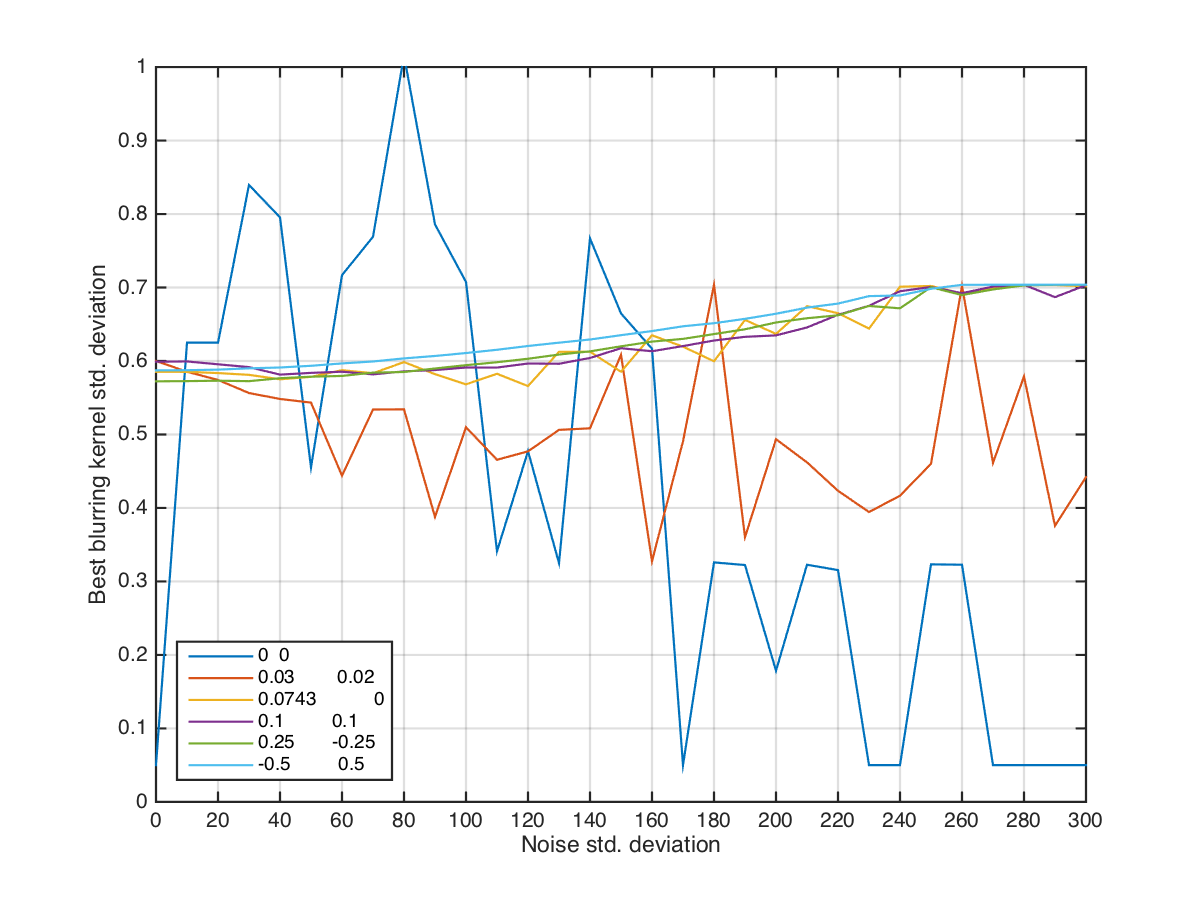
\includegraphics[width=1\textwidth]{Results/BestSigmaByShiftAndNoise}
	\caption{$\hat{\sigma}$ per noise}
\end{subfigure}	
\begin{subfigure}{0.45\textwidth}
	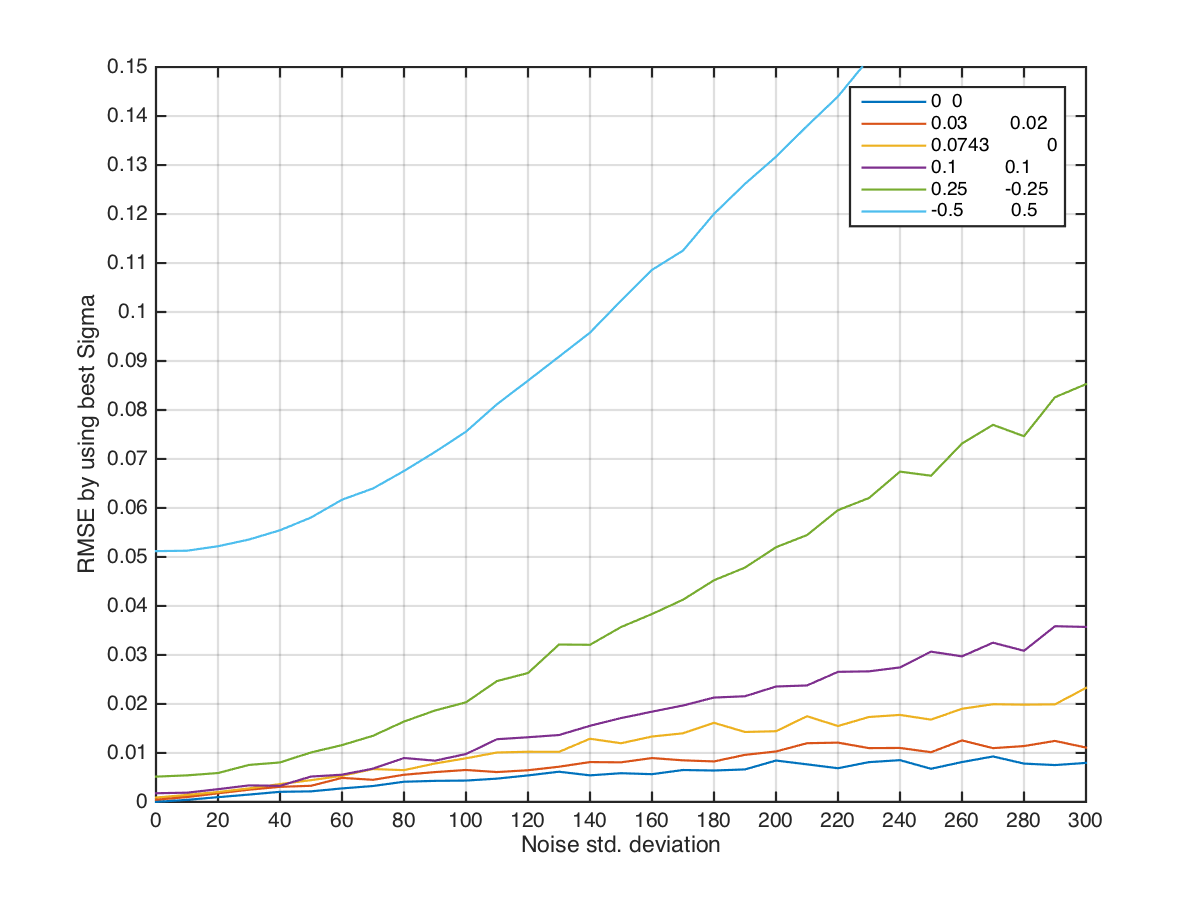
\includegraphics[width=1\textwidth]{Results/RMSEByShiftAndNoise}
	\caption{RMSE obtained using $\hat{\sigma}$}
\end{subfigure}	
\caption{$\hat{\sigma}$ values obtained based on noise and shift. Standard deviation of noise is considering 12-bit images.}
\label{fig:BestSigmaByNoiseAndShift}
\end{figure}

To better understand the importance of choosing the correct $\hat{\sigma}$, in Fig. \ref{fig:InfluenceOfSigmaByNoiseAndShift}, we performed two other experiments. In Fig. \ref{fig:avgStdDevOf10Best} the average standard deviation of the top 10 best RMSEs obtained by varying the $\sigma$ parameter is displayed, for each displacement. This implies to test each one of the values for the $\sigma$ parameter between $0$ and $1$ with step size of $0.05$, and obtain for each the resulting RMSE to finally compute the standard deviation of the lowest 10. For consistency, this experiment was averaged several times. As seen from the figure, the gain gets higher with the displacement magnitude. However, when the shift magnitude is under 0.1 pixels, this gain is negligible, suggesting in this case, a more relaxed selection of the $\sigma$ value.

%If instead of using Gaussian derivatives, the hypomode is used, the difference in accuracy is shown in Fig. \ref{fig:difWith0}. These results confirm the importance of applying a Gaussian prefilter to the images to estimate the gradients, in particular when the displacements are higher in magnitude than 0.1. For these cases, the accuracy gain is already 0.015 under low noise levels, and could potentially reach as high as a sixth of a pixel for higher displacements values. 

Finally, since $\sigma=0.6$ usually achieved good results, a comparison between the best $\hat{\sigma}$ and $\sigma=0.6$ was made in Fig.~\ref{fig:difWith06}. Interestingly, by fixing $\sigma=0.6$, higher accuracy gains could be obtained when the displacements are of small magnitude (lower than 0.1 pixels). However, when the displacement is high enough (in our case half a pixel in magnitude), under low SNR values (noise std. dev. bigger than 150), the accuracy gain by selecting the correct $\hat{\sigma}$ could be as high as 0.016 pixels. This implies that for low displacement magnitudes, lower $\sigma$ values should be used (around $\sigma=0.45$); for medium shift magnitudes (between 0.1 and 0.3); $\sigma=0.6$ should be used, and for high displacements, the decision to increase the $\sigma$ relies on the noise level.


\begin{figure}[!ht]
	\centering
	\begin{subfigure}{0.45\textwidth}
		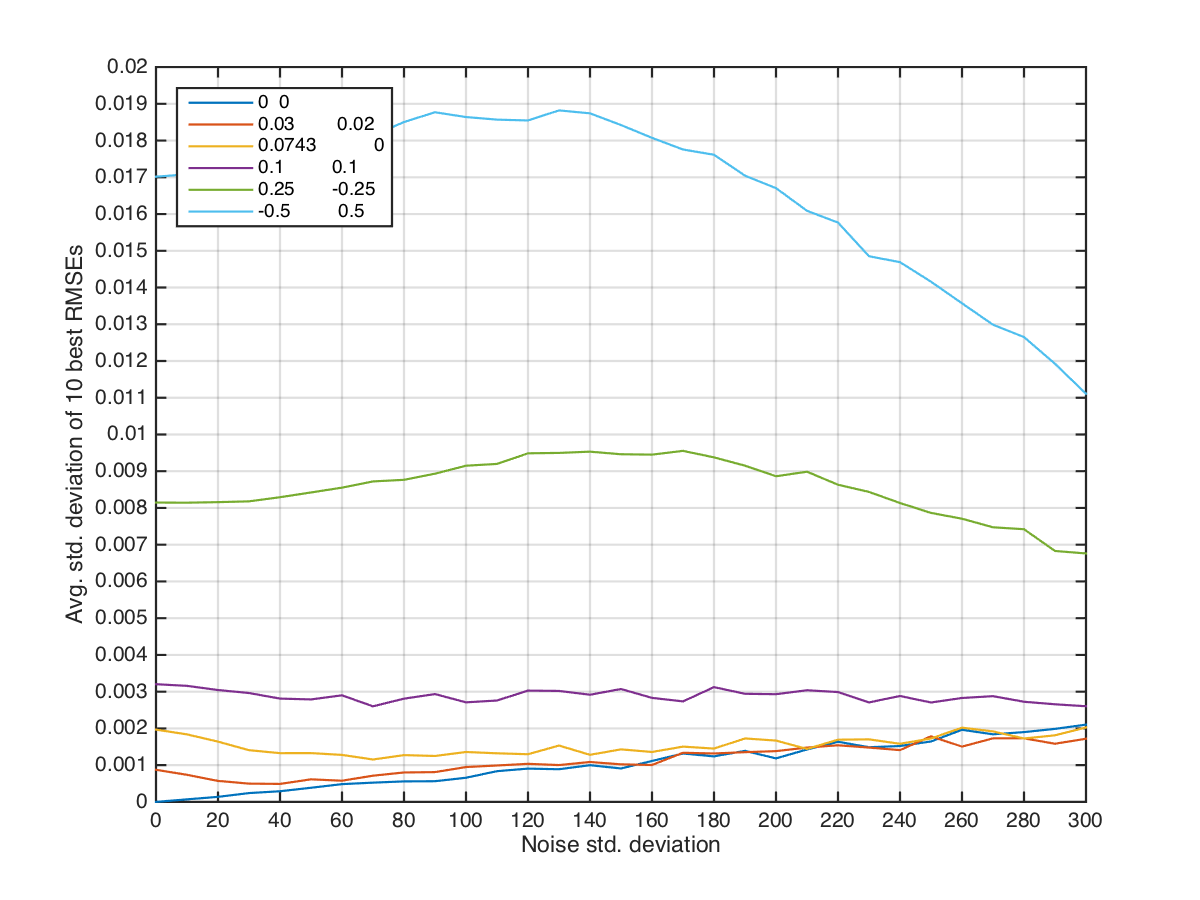
\includegraphics[width=\textwidth]{Results/avgStdOf10BestByShiftAndNoise}
		\caption{Average standard deviation of ten\\ best RMSEs per shift}
		\label{fig:avgStdDevOf10Best}
	\end{subfigure}
%	\quad
%	\begin{subfigure}{0.31\textwidth}
%		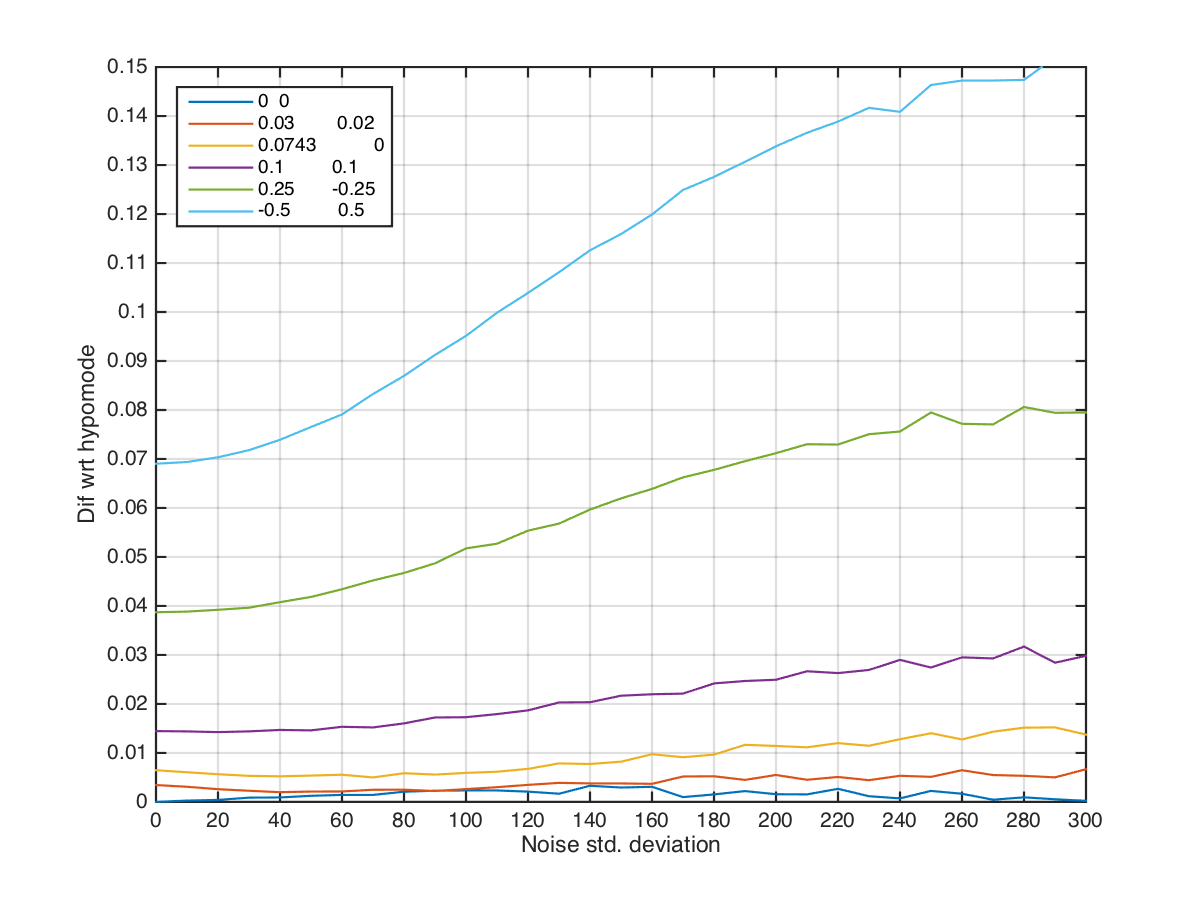
\includegraphics[width=1\textwidth]{Results/DifWith0ByShiftAndNoise}
%		\caption{Difference between RMSE obtained using $\hat{\sigma}$ and using the hypomode}
%		\label{fig:difWith0}
%	\end{subfigure}
%	\quad
	\begin{subfigure}{0.45\textwidth}
		 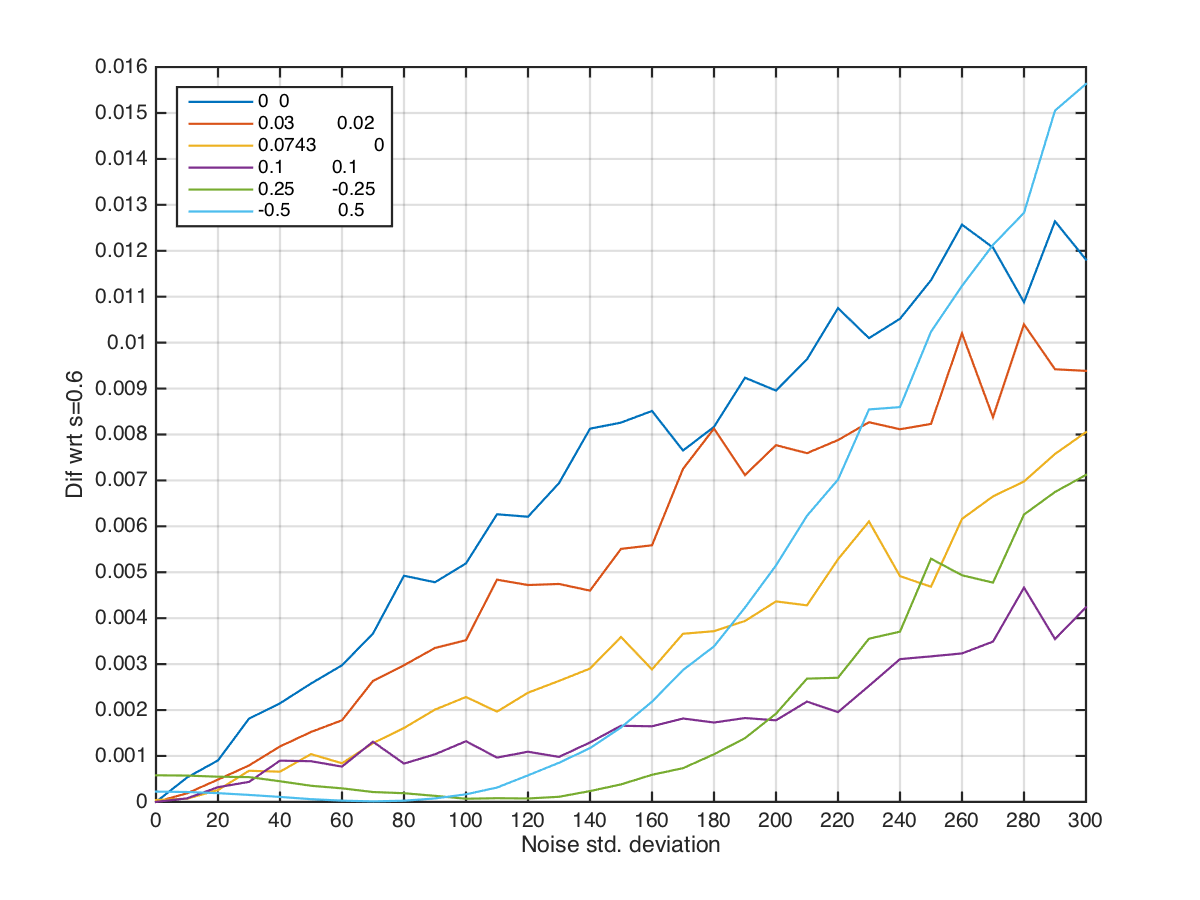
\includegraphics[width=1\textwidth]{Results/DifWith06ByShiftAndNoise}
		 \caption{Difference between RMSE obtained using $\hat{\sigma}$ and using the $\sigma=0.6$}
		 \label{fig:difWith06}
	\end{subfigure}
	\caption{Influence of using the correct $\sigma$ for the Gaussian kernel on the results}
	\label{fig:InfluenceOfSigmaByNoiseAndShift}
\end{figure}


Another experiment was performed to confirm the $\hat{\sigma}$ values obtained under different image conditions. Three image types were selected, namely a textured image, a low SNR image, and an image having the well-known aperture problem (the gradient direction is mostly uniform across the image). Also, larger shifts up to $\norm{v} = 1$ were included for this test. Results averaging all evaluated shifts are displayed in Fig.~\ref{fig:BestSigmaByImageTypeAndNoise}. It seems that for well-textured images, values of $\sigma$ between 0.6 and 0.8 achieved the best performance, however for more complicated images, higher values achieved better results. This makes sense, since in a case where high precision is not possible, considerably blurring the image decreases the maximum shift returned and therefore the maximum error. This can be seen in Fig.~\ref{subfig:BestSigmaByImageTypeAndNoiseB} where the average errors reach almost half the magnitude and the largest evaluated shift. 
\begin{figure}[!ht]
	\centering
	\begin{subfigure}{0.45\textwidth}
	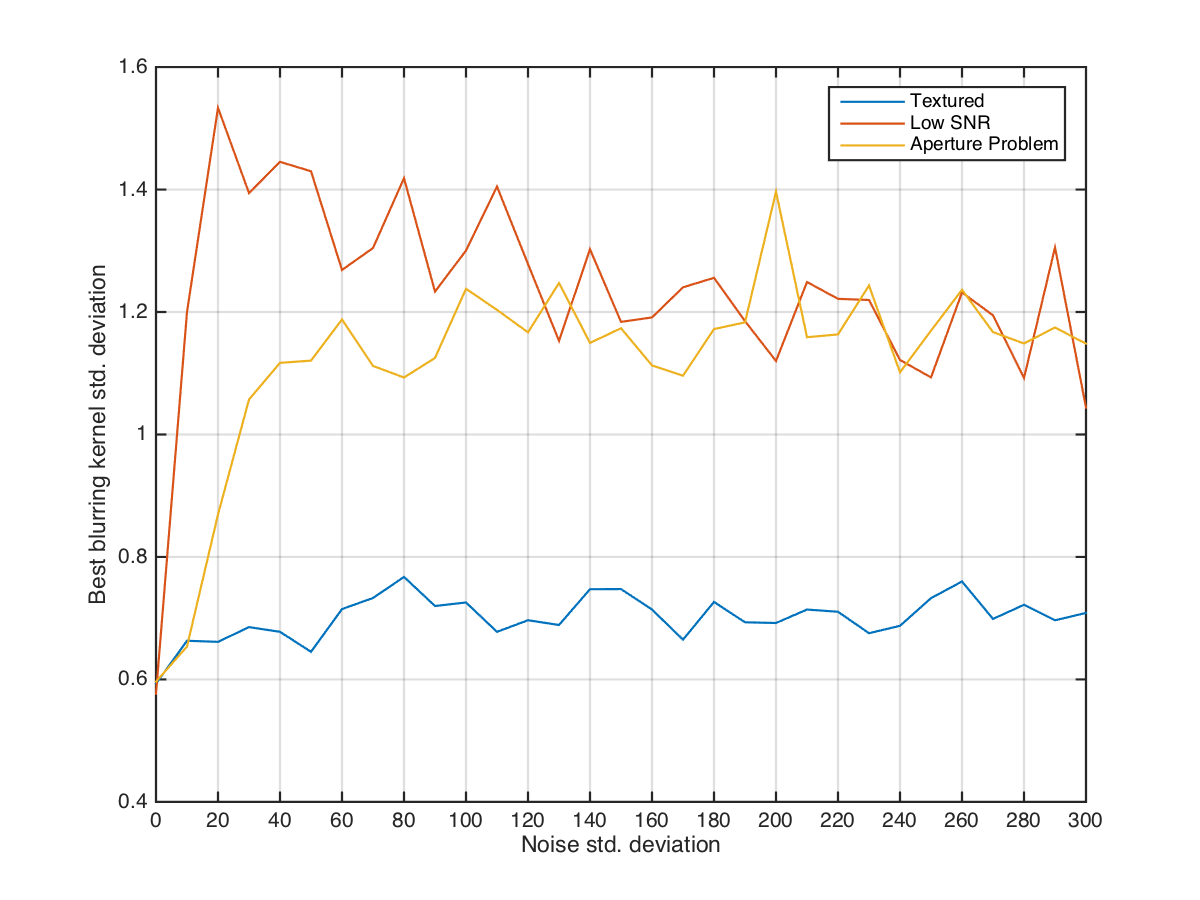
\includegraphics[width=1\textwidth]{Results/BestSigmaByImageTypeAndNoise}
	\caption{$\hat{\sigma}$ per noise}
	\end{subfigure}
	\begin{subfigure}{0.45\textwidth}
	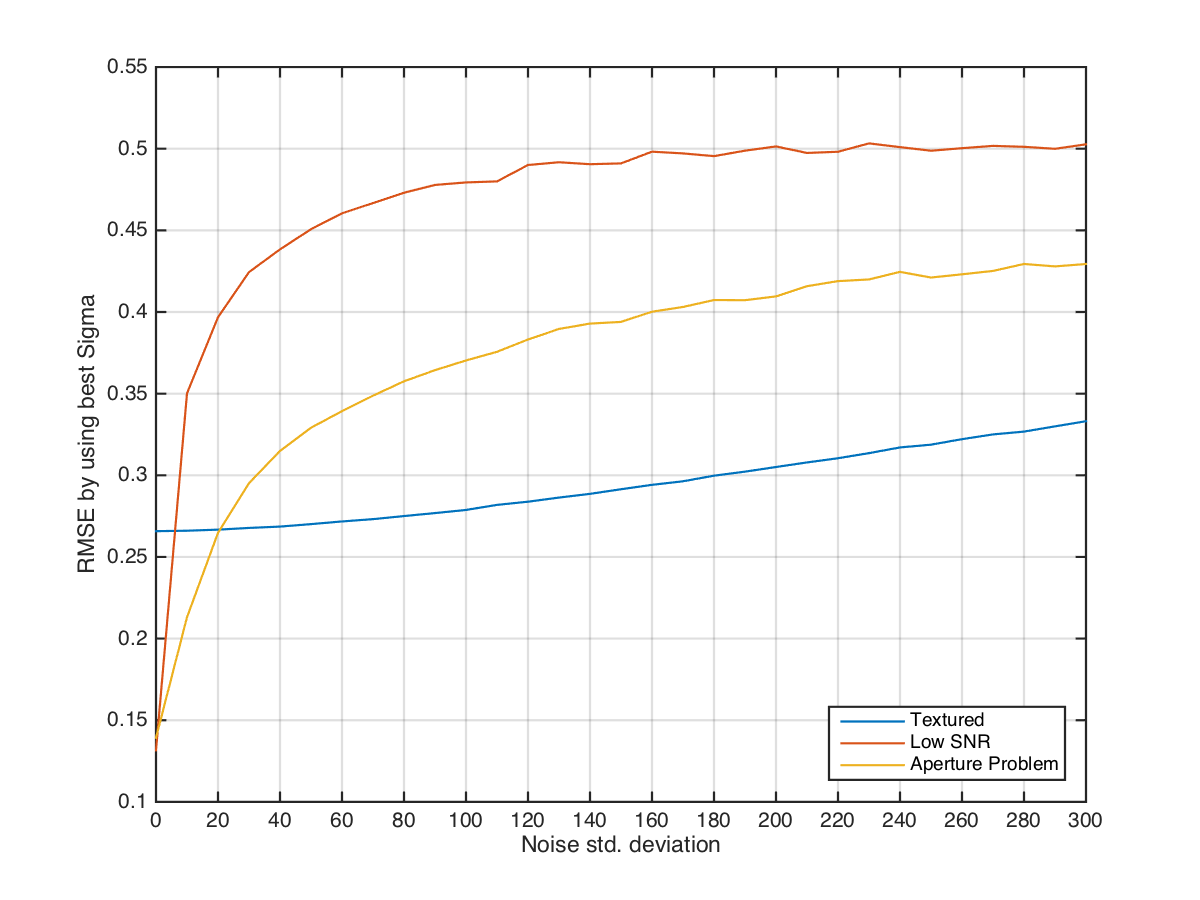
\includegraphics[width=1\textwidth]{Results/RMSEByImageTypeAndNoise}
	\caption{RMSE of methods using $\hat{\sigma}$}
	\label{subfig:BestSigmaByImageTypeAndNoiseB}
	\end{subfigure}
	\caption{$\hat{\sigma}$ values obtained based on problematic case and noise.}
	\label{fig:BestSigmaByImageTypeAndNoise}
\end{figure}
It has to be noted that for each noise amount, each problematic case and each simulated shift, a total of 1000 experiments were performed. The $\hat{\sigma}$ displayed on the figures is the median while the RMSE shown is the average RMSE of these experiments.

Finally, to give more insight about the progression of the error based on the blurring kernel standard deviation used and on the noise, Fig.~\ref{fig:RMSEPerBlurAndNoise} shows the RMSE, in pixels, depending on the underlying shift to be estimated. As it can be seen from the graphs, as the noise increases, also does the error, as expected, and the $\hat{\sigma}$ that minimizes this error seems to be around 0.6, growing as high as 0.7 when the noise becomes high. Another interesting result is that as the displacement grows, the fact that values of $\hat{\sigma}$ around 0.6 are the best becomes more apparent. However, when the shift is small enough (lower than 0.1 pixel), other $\hat{\sigma}$ values should be used, as remarked in the previous test. Furthermore, for the case of high shift magnitude and high noise, the estimation error becomes higher, so accurately setting $\sigma$ in these cases could be justified by the accuracy gain.

\begin{figure}[!ht]
	\centering
	\begin{subfigure}{0.45\textwidth}
	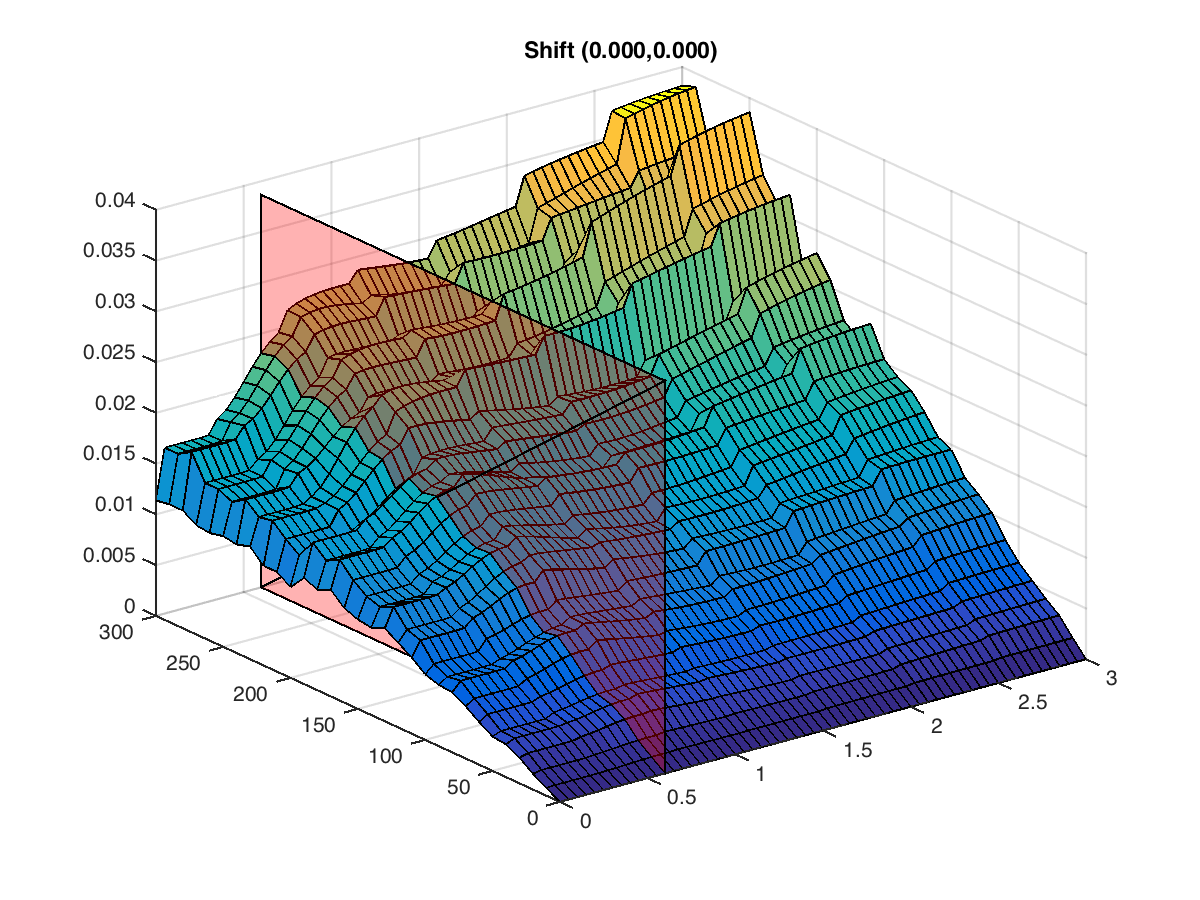
\includegraphics[width=1\textwidth]{Results/ErrorByBlurAndNoiseForShift1}
	\caption{Shift (0,0)}
	\end{subfigure}	
	\begin{subfigure}{0.45\textwidth}
	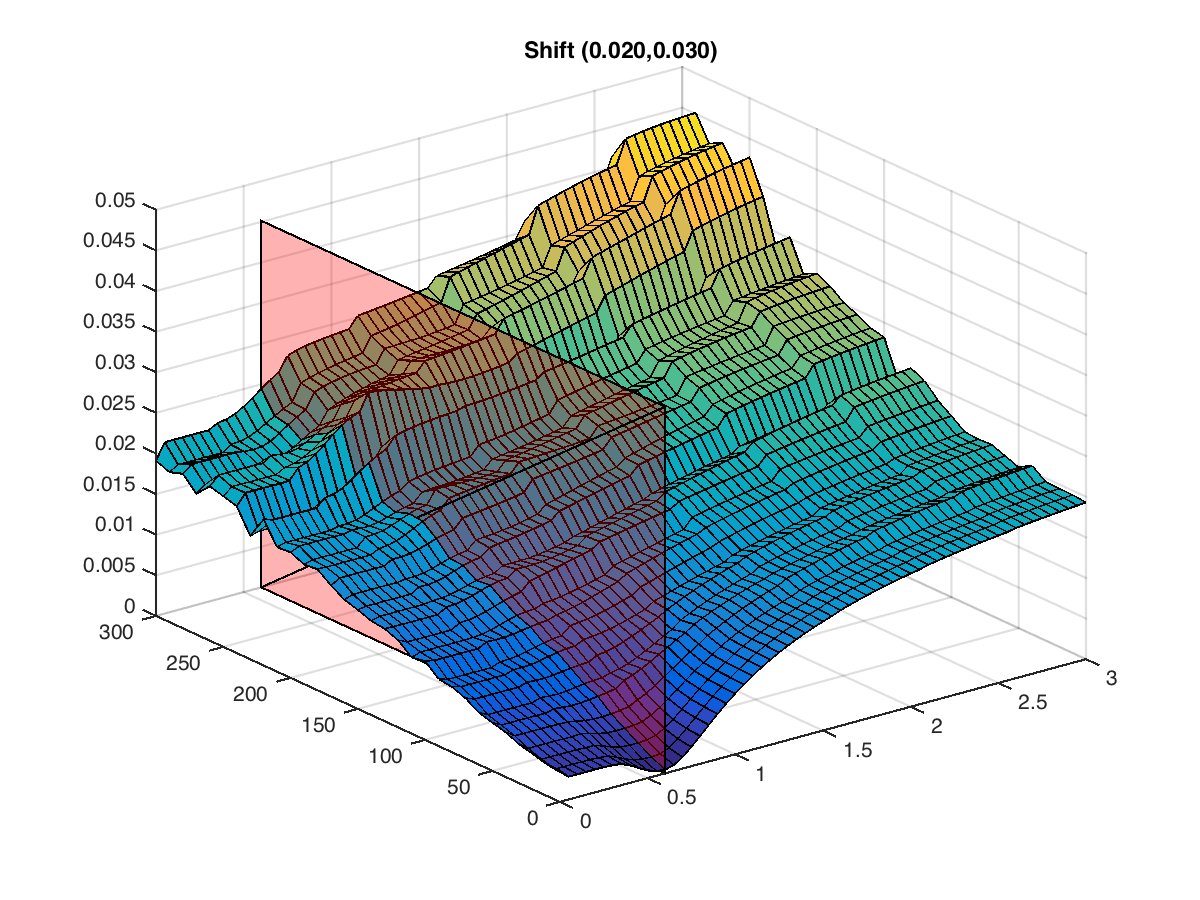
\includegraphics[width=1\textwidth]{Results/ErrorByBlurAndNoiseForShift2}
	\caption{Shift (0.02, 0.03)}
	\end{subfigure}	
	\quad
	\begin{subfigure}{0.45\textwidth}
		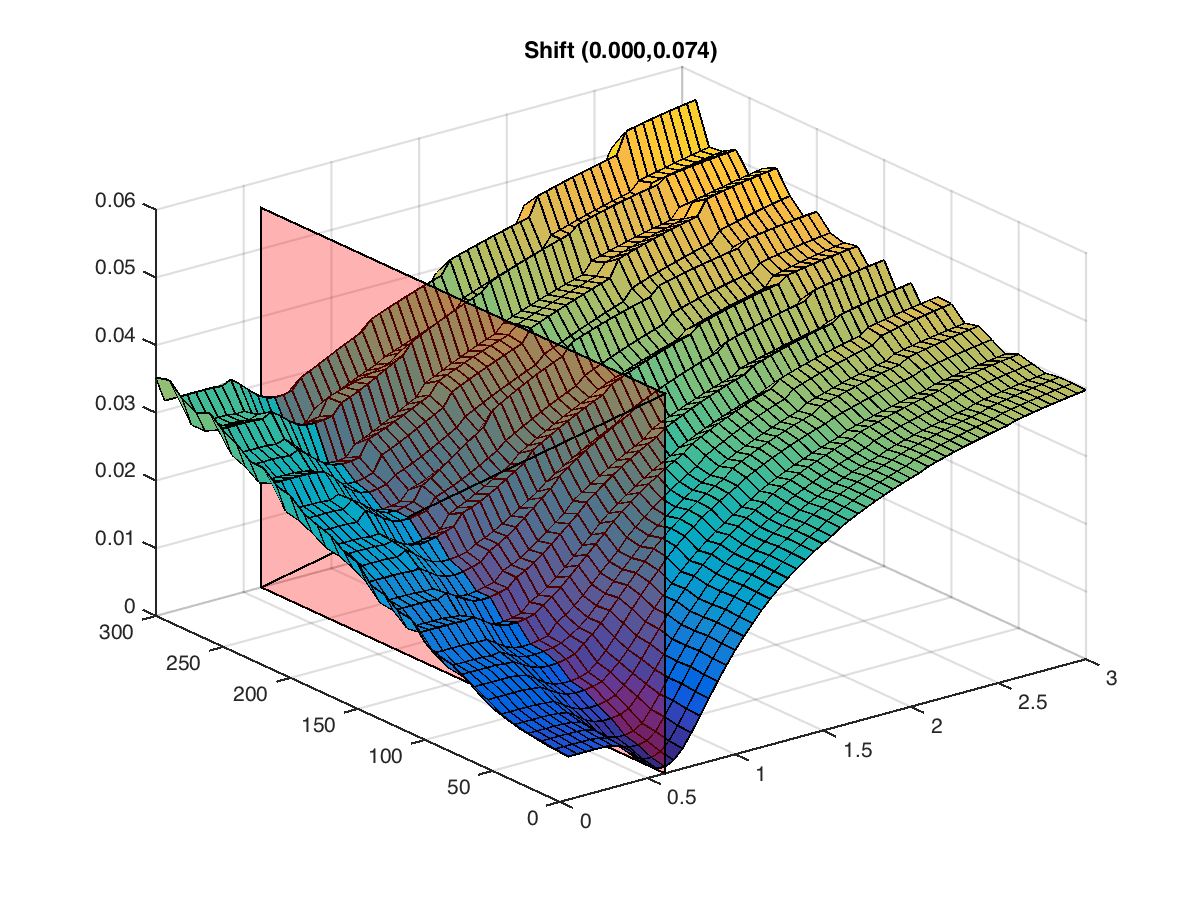
\includegraphics[width=1\textwidth]{Results/ErrorByBlurAndNoiseForShift3}
		\caption{Shift (0, 0.074)}
	\end{subfigure}
	\begin{subfigure}{0.45\textwidth}
		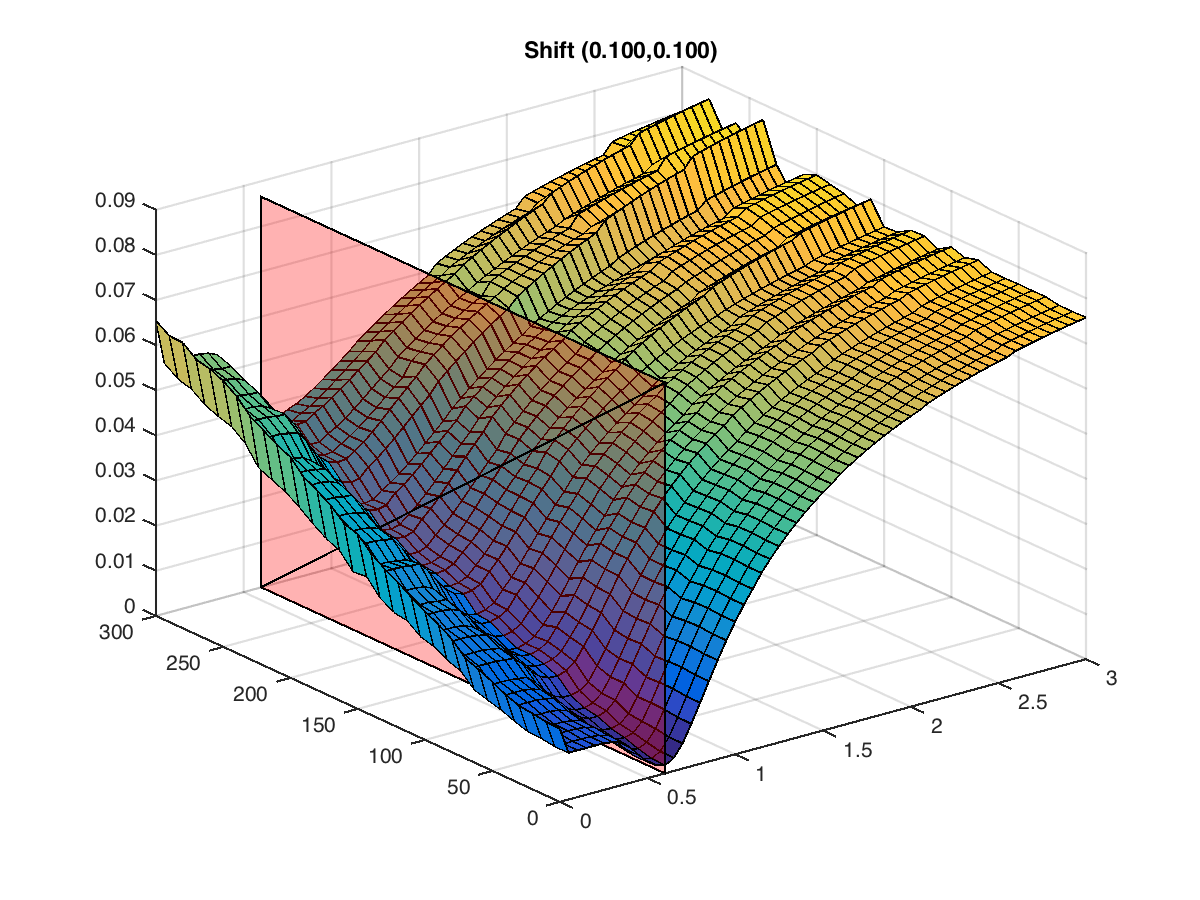
\includegraphics[width=1\textwidth]{Results/ErrorByBlurAndNoiseForShift4}
		\caption{Shift (0.1, 0.1)}
	\end{subfigure}	
	\quad
	\begin{subfigure}{0.45\textwidth}
		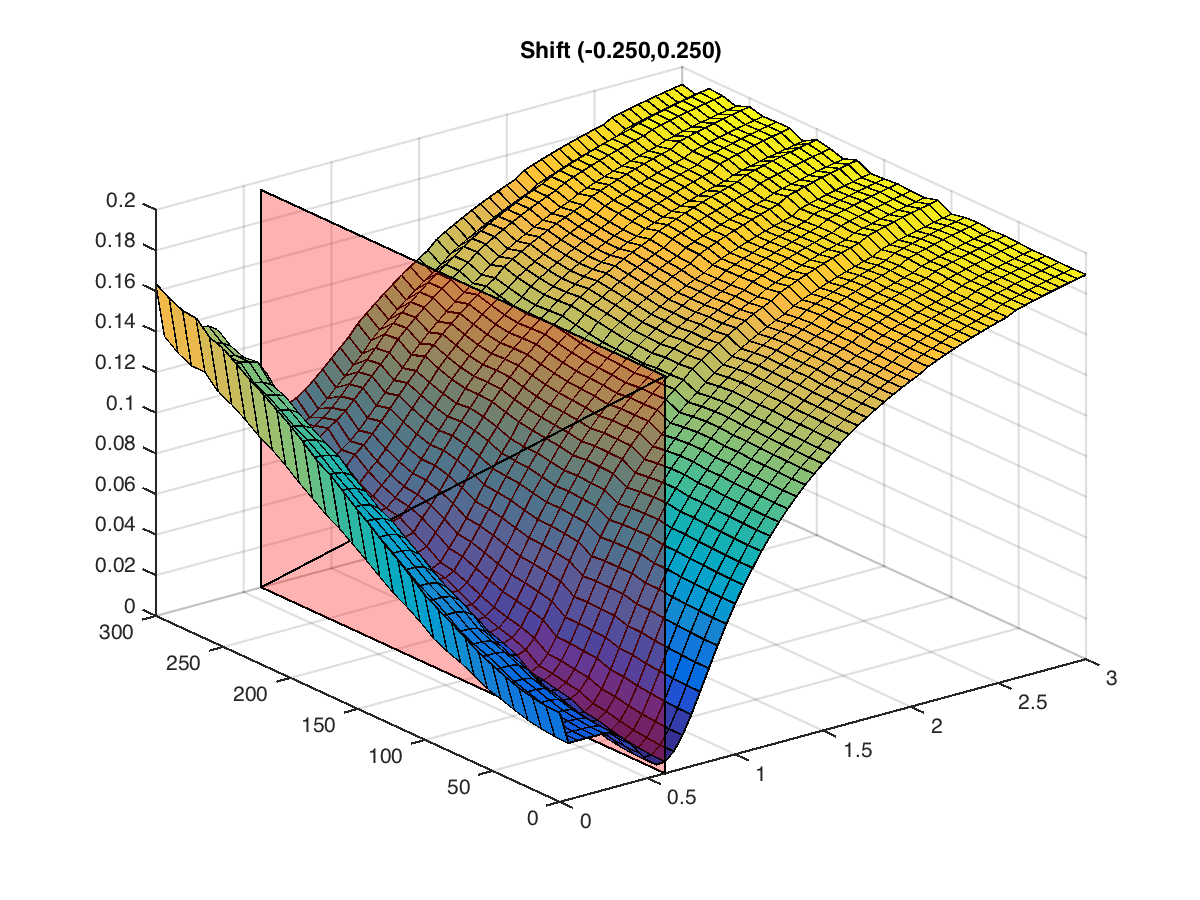
\includegraphics[width=1\textwidth]{Results/ErrorByBlurAndNoiseForShift5}
		\caption{Shift (-0.25, 0.25)}
	\end{subfigure}	
	\begin{subfigure}{0.45\textwidth}
		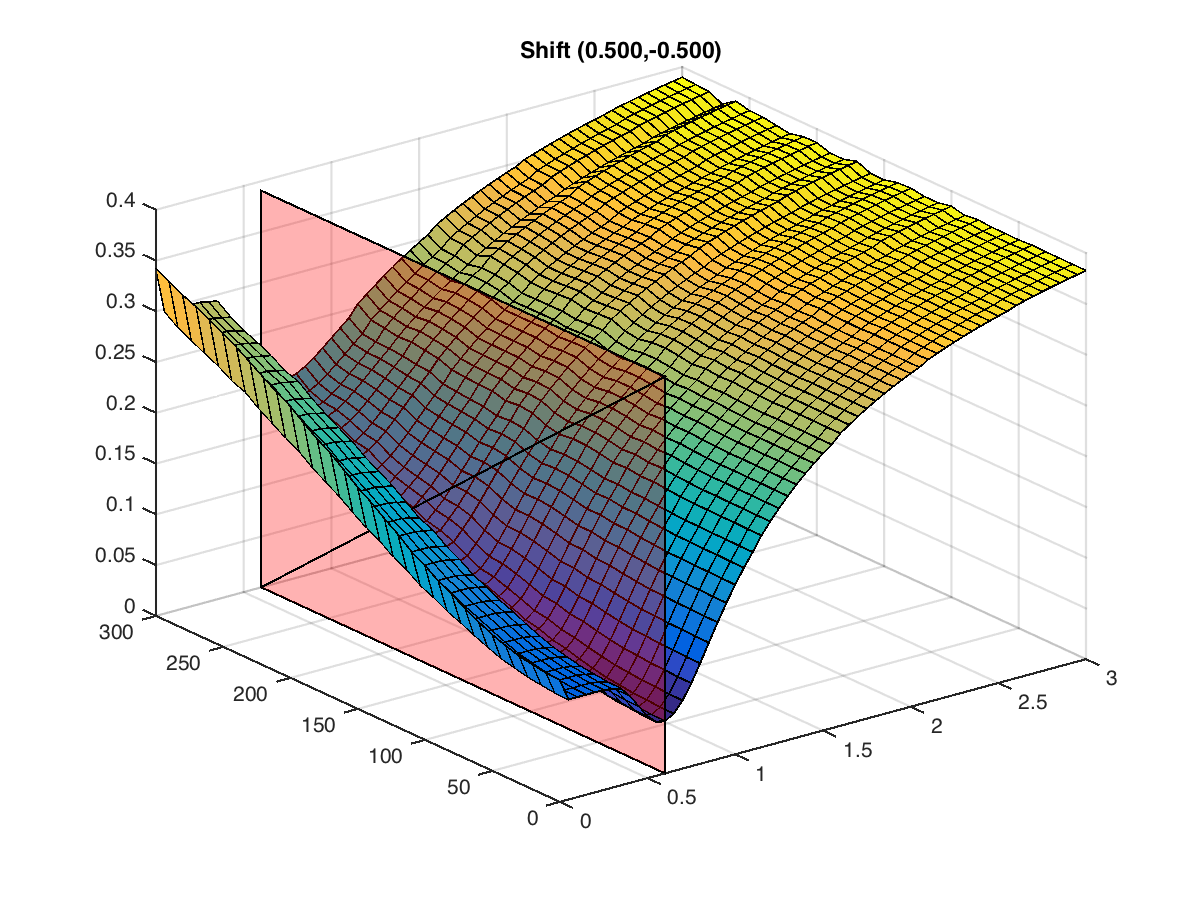
\includegraphics[width=1\textwidth]{Results/ErrorByBlurAndNoiseForShift6}
		\caption{Shift (0.5, -0.5)}
	\end{subfigure}	
	\caption{Evolution of RMSEs obtained based on $\hat{\sigma}$ values (from 0 to 3) and noise (from $0$ to $300$] for each shift. The red rectangle shows, as a reference, $\sigma=0.6$. }
	\label{fig:RMSEPerBlurAndNoise}
\end{figure}

\clearpage

\subsection{Robustness to noise}
One of the most important difficulties in shift estimation is related to the presence of noise on the input images. In this section, we evaluate the effects of noise on each method in a simulated environment. For each error value shown, an average of 100 experiments was performed, each time generating a new noise realization and using a different random subimage. Due to the randomness of the  experiment, potential content-less images or aperture problem cases could exist. However, by using validation methods such as the Cramer-Rao lower bound, these cases were excluded from the results and the computed averages were based on valid cases only. Note also that by selecting random subimages, two experiments with injected noise sharing the same standard deviation could still have different SNRs. This was on purpose, to evaluate the versatility of each method under potentially plausible situations.

%To evaluate the performance for each method under Gaussian noise, two experiments were performed. In both cases, an image is extracted from a high resolution noiseless image and shifted. White Gaussian noise is later added to both images, the original and its shifted version. Several shift values were used to evaluate the performance for each method: (0,0.0745), (0.5,0.5), (0.9,0.1), (0,0.75), (0.5, -0.5), (0.9, 0.5), (0, 0), (0.2, -0.2), (0.01, 0), (0.3, 0.3), (0.024, 0.052) and (-0.7, 0.7). Also, the noise level, starting at $\sigma=1$, was increased each time by 20 ending at $\sigma=481$, where images were visibly heavily corrupted by noise.
%\subsubsection{Robustness to noise depending on the shift magnitude}
As proved by both Robinson \cite{Robinson2004} and Pham \cite{pham2005performance}, the negative effect of noise is stressed as the displacement to estimate gets larger. For this reason, we evaluated the performance of every approach by varying noise and displacement magnitude conditions, based on the noise levels shown in Table \ref{tab:noiseLevels}. Figure \ref{fig:exampleSimulatedNoisyLevels} shows an example of two landscapes, the first with high photon count and the second with average photon count, under each simulated noise level. While in the first landscape, the effects of the noise start to be noted from the third noise level, for the second case it is already noticeable on the second level.


\begin{figure}[htpb]
\begin{subfigure}{.2\textwidth}
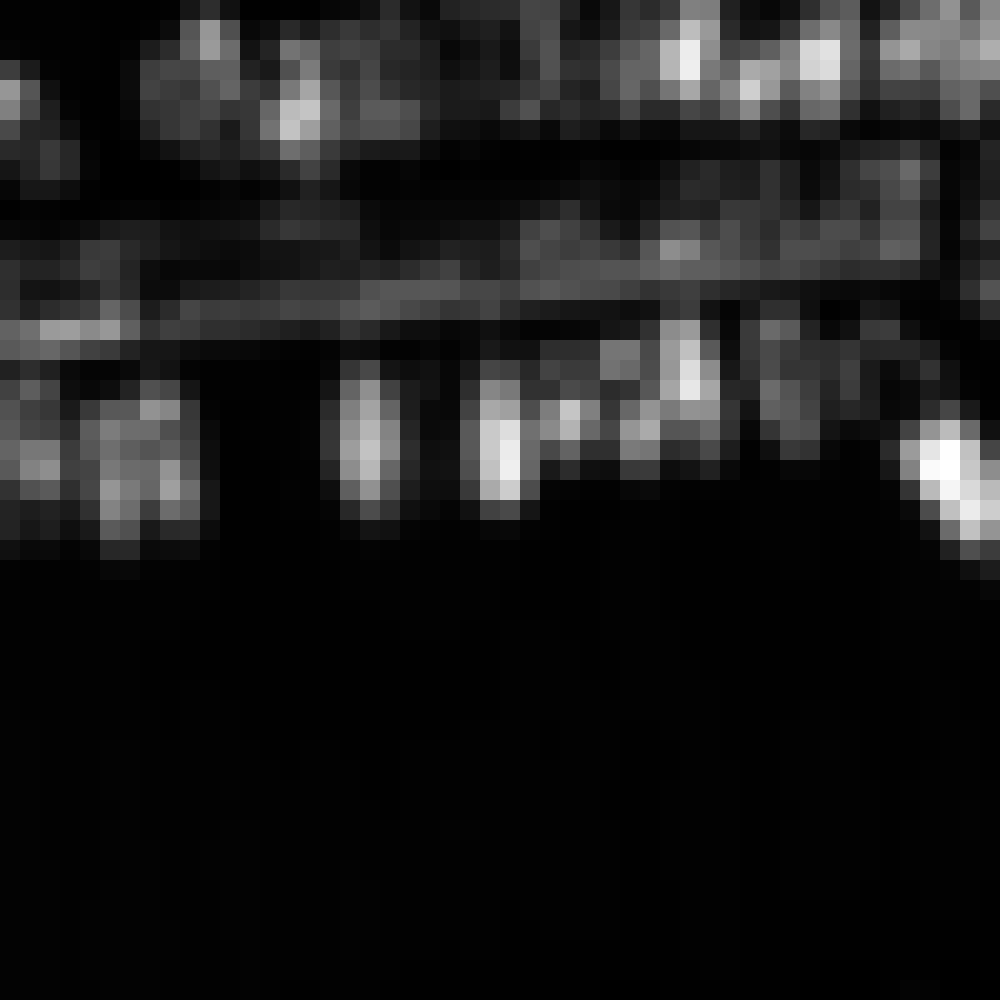
\includegraphics[width=\textwidth]{img/image2NoiseLevel1}
\end{subfigure}%
\begin{subfigure}{.2\textwidth}
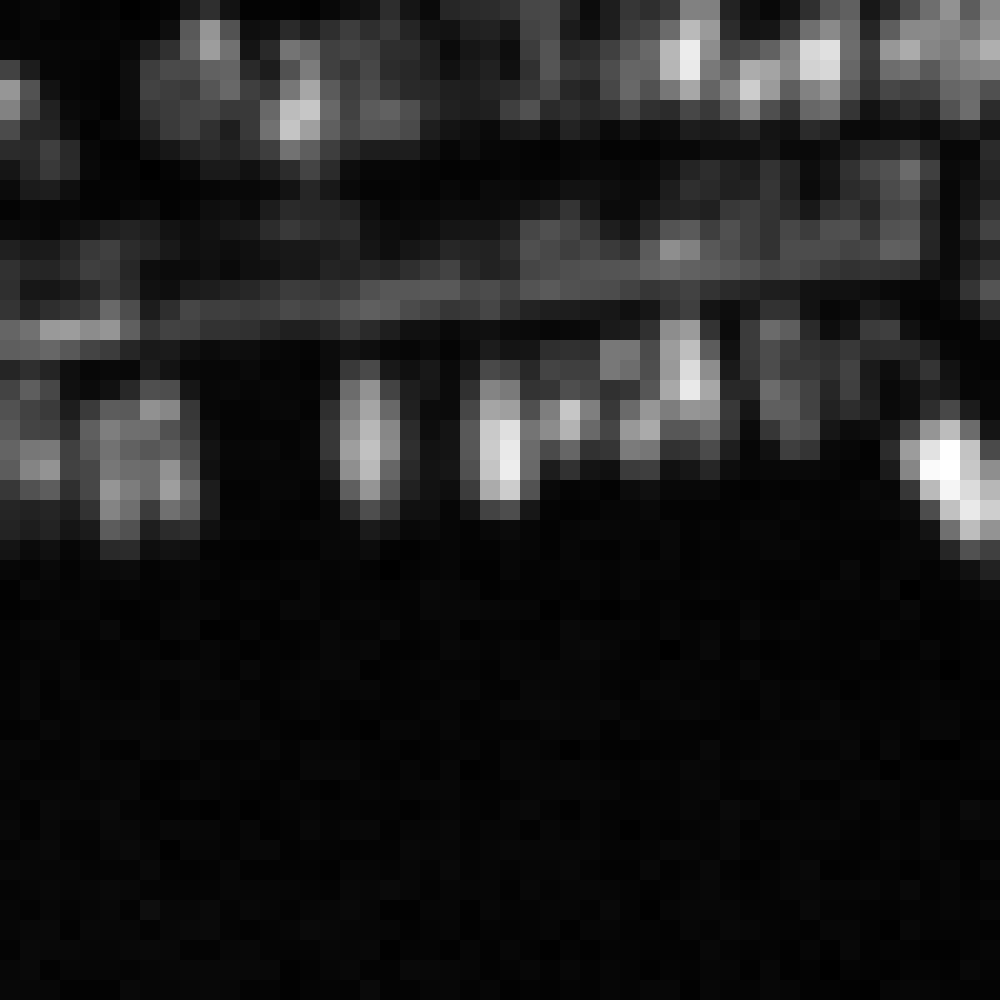
\includegraphics[width=\textwidth]{img/image2NoiseLevel2}
\end{subfigure}%
\begin{subfigure}{.2\textwidth}
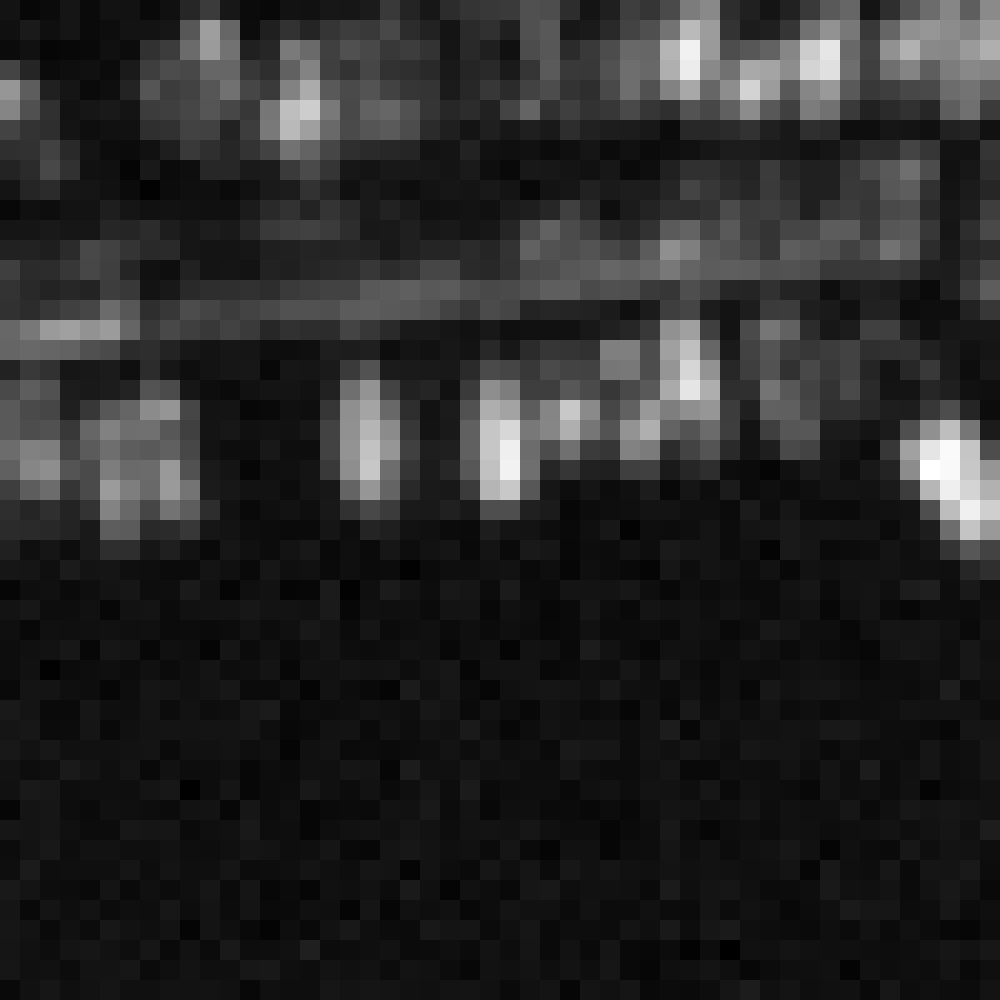
\includegraphics[width=\textwidth]{img/image2NoiseLevel3}
\end{subfigure}%
\begin{subfigure}{.2\textwidth}
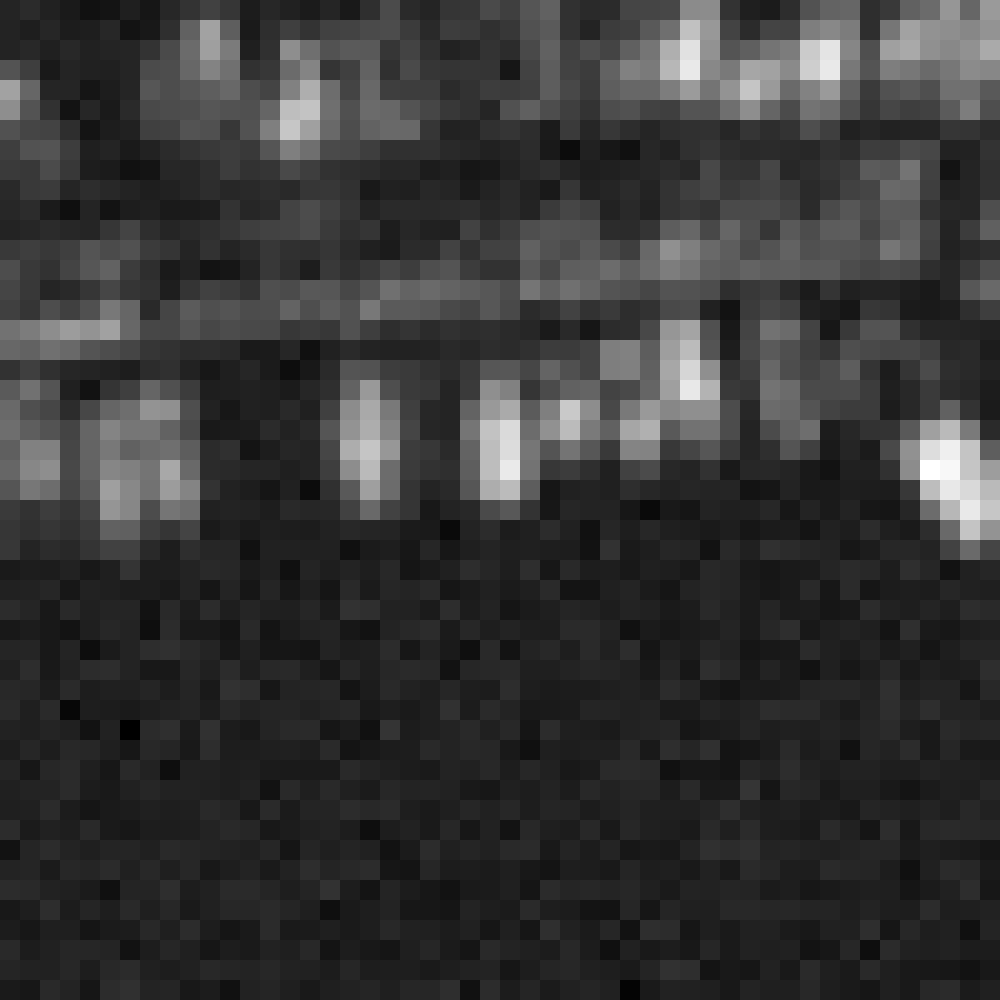
\includegraphics[width=\textwidth]{img/image2NoiseLevel4}
\end{subfigure}%
\begin{subfigure}{.2\textwidth}
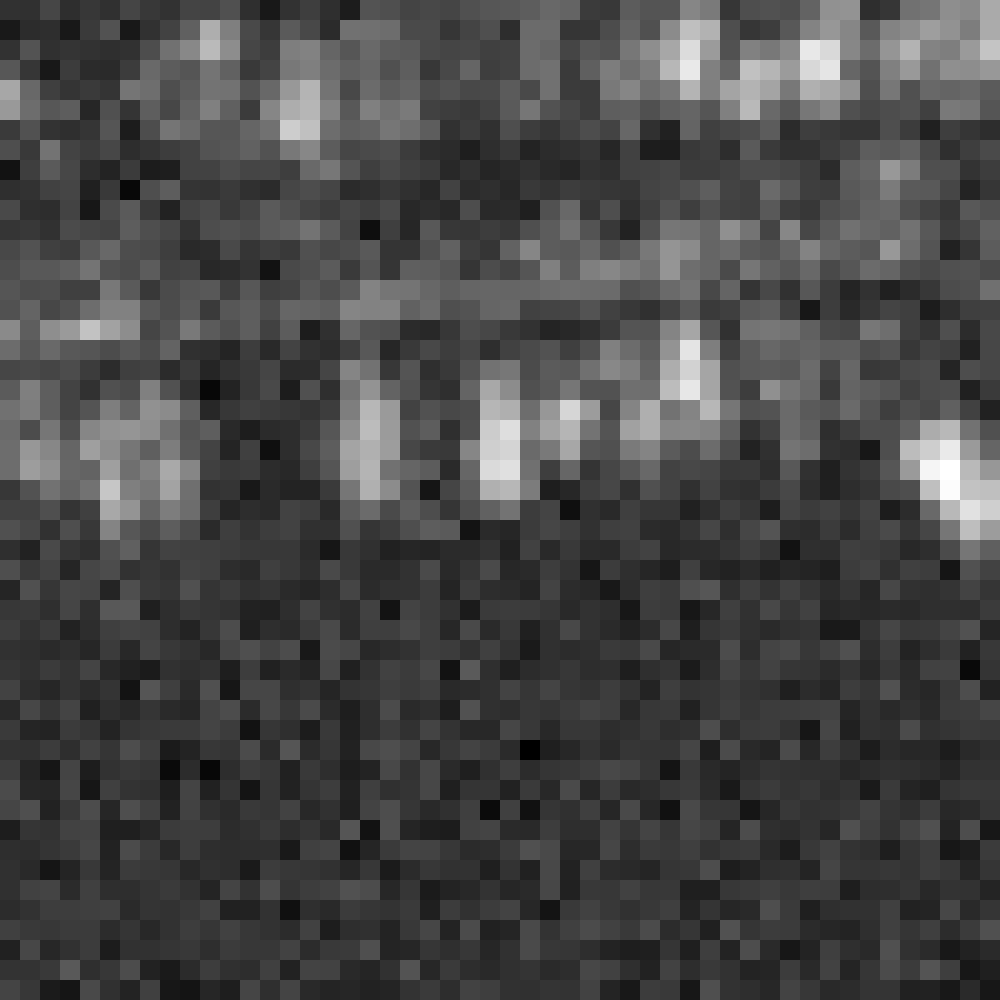
\includegraphics[width=\textwidth]{img/image2NoiseLevel5}
\end{subfigure}
\quad
\begin{subfigure}{.2\textwidth}
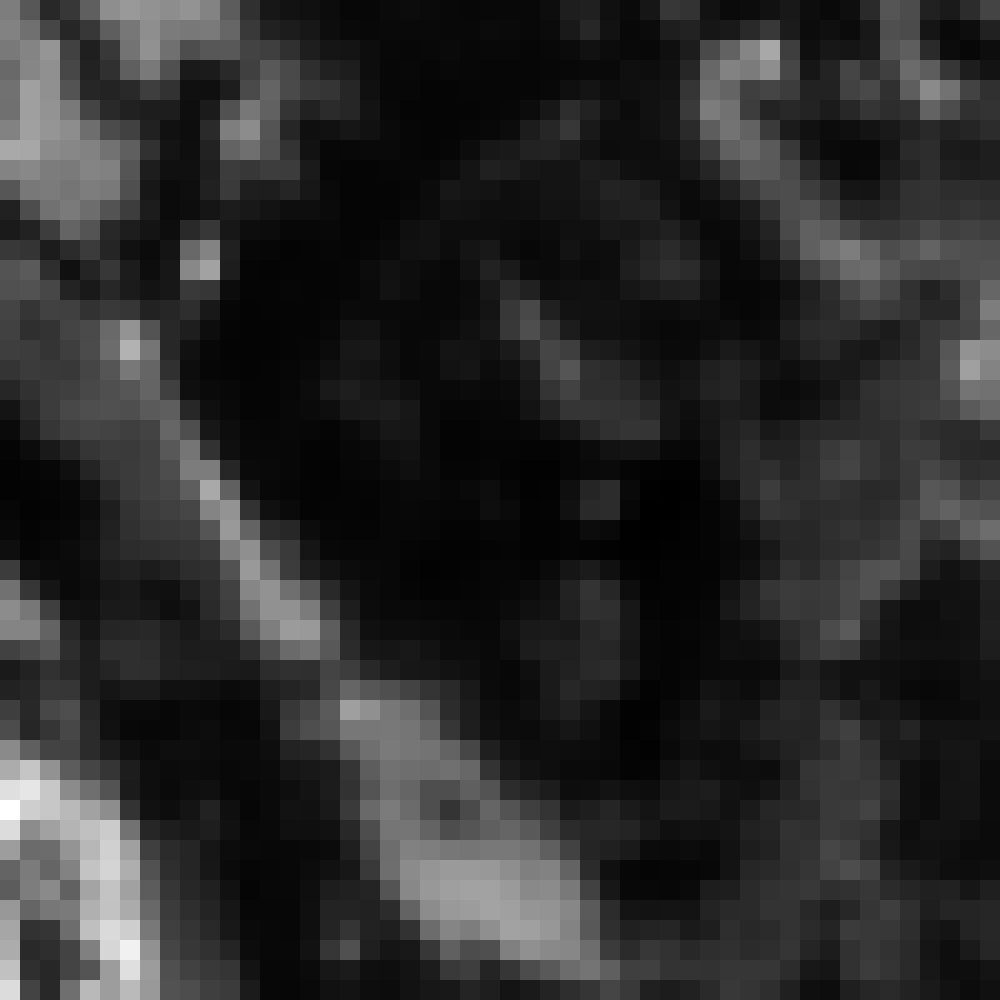
\includegraphics[width=\textwidth]{img/imageNoiseLevel1}
\caption{Level 1}
\end{subfigure}%
\begin{subfigure}{.2\textwidth}
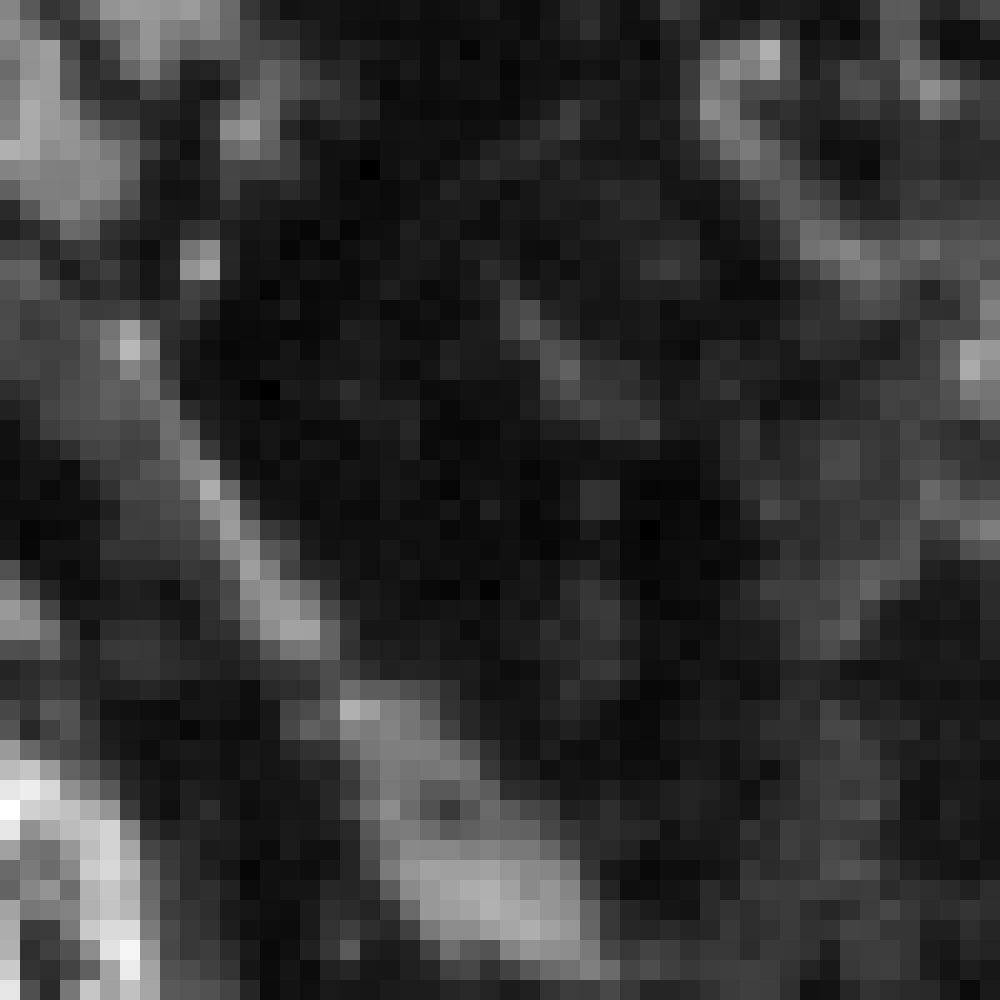
\includegraphics[width=\textwidth]{img/imageNoiseLevel2}
\caption{Level 2}
\end{subfigure}%
\begin{subfigure}{.2\textwidth}
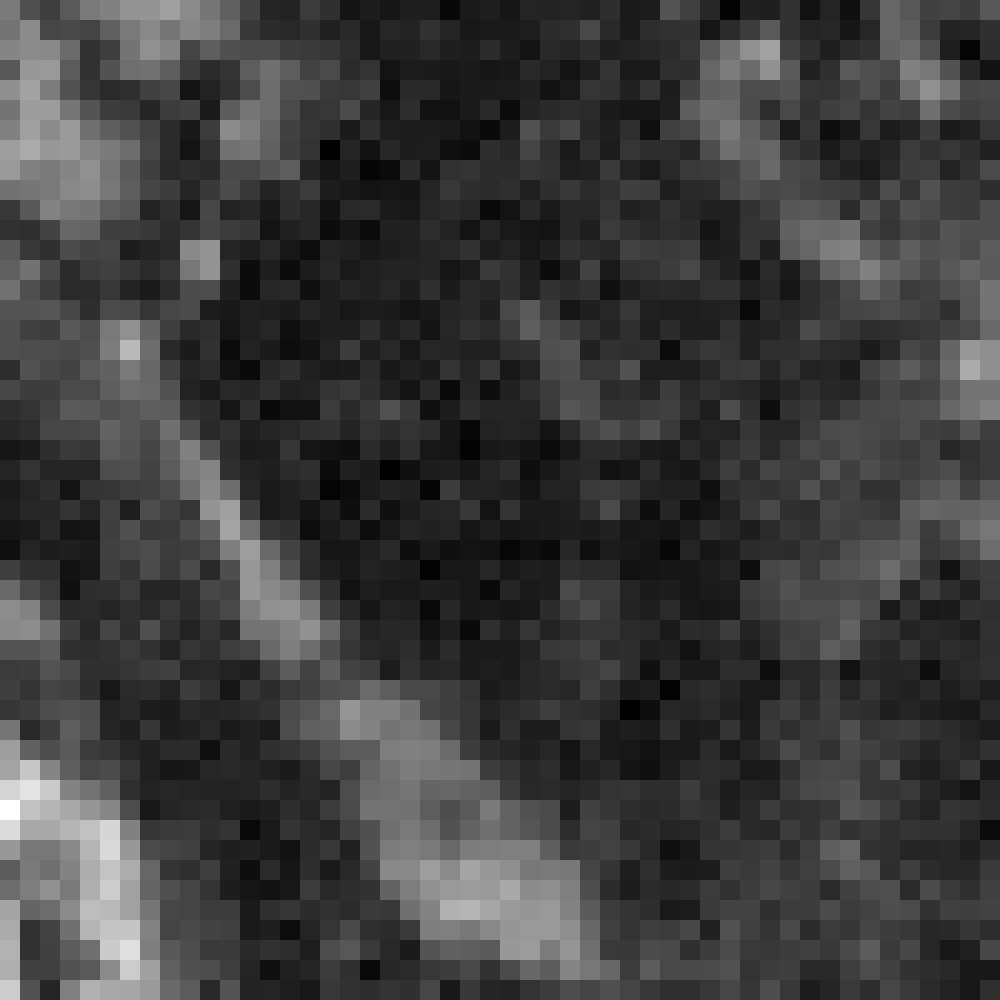
\includegraphics[width=\textwidth]{img/imageNoiseLevel3}
\caption{Level 3}
\end{subfigure}%
\begin{subfigure}{.2\textwidth}
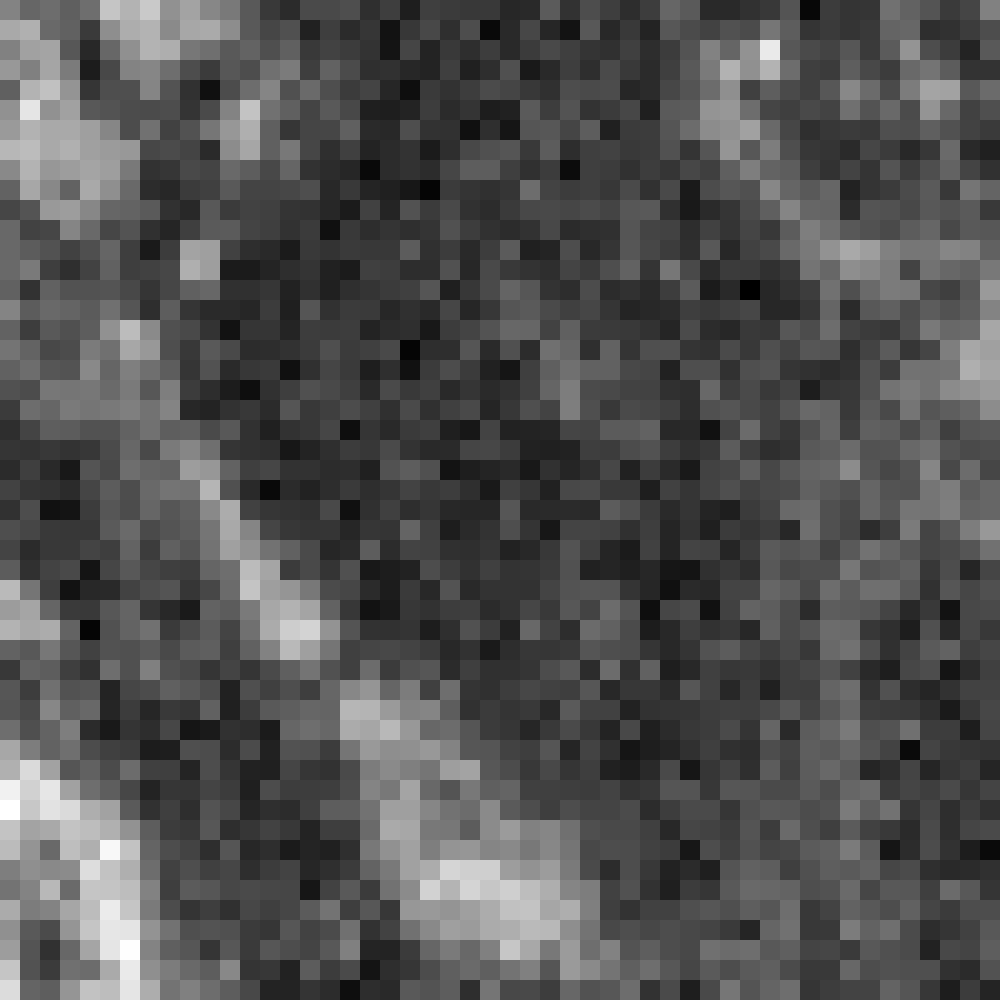
\includegraphics[width=\textwidth]{img/imageNoiseLevel4}
\caption{Level 4}
\end{subfigure}%
\begin{subfigure}{.2\textwidth}
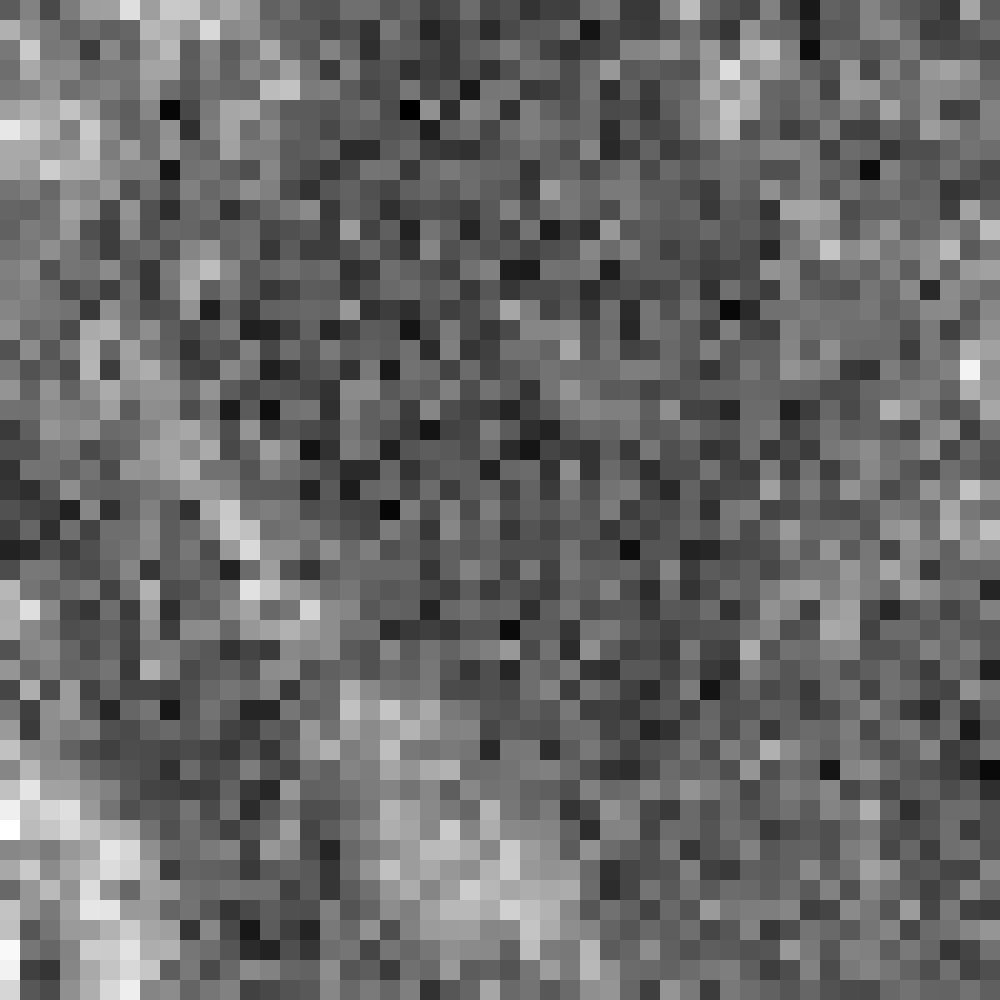
\includegraphics[width=\textwidth]{img/imageNoiseLevel5}
\caption{Level 5}
\end{subfigure}
\caption{Sample images for the five analyzed noise levels. \textbf{Top}: high constrasted image (high SNR). \textbf{Bottom}: intermediate contrasted image (average SNR). Dynamic ranges extended for visualization purposes.}
\label{fig:exampleSimulatedNoisyLevels}
\end{figure}


%In the same manner, several displacements were tested and results were grouped into 4 categories. The reason behind this distinction is that some methods are more suited than others for each designated category. The ranges for each shift magnitude level are as shown in table \ref{tab:shiftMagnitudeCategories}. In the first category, extremely small sub-pixelian shifts were considered, as they could exist in several applications, for example the Stav-Active problem presented in chapter 3 of this thesis. We also include as a fourth category, magnitudes larger than 1.1 pixels. By design, all non-multiscale GBSE methods as well as the phase correlation method from Stone \cite{Stone_2001} fail under this category. Due to this reason, although being shown for completeness, this shift magnitude is excluded from the general averages.
%
%\begin{table}[htpb]
%\centering
%\begin{tabular}{|c|c|c|c|c|} 
%	\hline
%	Level & 1 & 2 & 3 & 4 \\ \hline
%	Range & $\norm{\bv} \leq 0.1$ & $0.1 < \norm{\bv} \leq 0.5$ & $0.5 < \norm{\bv} \leq 1.1$ & $\norm{\bv} > 1.1$ \\ \hline
%\end{tabular}
%\caption{Shift magnitude ($\norm{\bv}$) ranges for each evaluated category.}
%\label{tab:shiftMagnitudeCategories}
%\end{table}

To summarize results, we display in Table \ref{tab:top10NoiseAndShiftAllVariants} the top 10 methods together with their average errors for each evaluated shift magnitude category and every noise level analyzed. Also, the averages by noise level and by shift magnitude were included in the results. Since in general each top 10 is dominated by the different variants from a single method, this table does not seem too informative. However, some interesting conclusions could be inferred. First, the best methods are always gradient-based, and the amount of iterations and/or scales depends on the shift magnitude. For the lowest shift magnitude studied, using a single or two iterations of the original LS or the TLS method are optimal. For the second analyzed magnitude category, the best results were obtained without requiring a multiscale approach, however several iterations should be performed (three or four). Finally, for the remaining shift magnitudes, a multiscale approach is mandatory and the configuration that seems to achieve the best results is to start with a single iteration on the broadest scale and increasing the amount of iterations by one for each subsequent scale progressively. Also, for the finest scale, the best interpolation scheme should be used (FFT with or without symmetrization or spline). Finally, for short shift-magnitudes, the gradients with the smallest supports are recommended. In particular, the hypomode stands out from the rest. As the shift magnitude increases, both  $3\times 3$ Farid or Simoncelli gradient estimation methods attain better scores under lower SNR scenarios. As a special case, under infinite SNR situations, larger gradient estimation kernels seem to achieve the best accuracies.

\begin{table}[htpb]
\scriptsize
\setlength{\tabcolsep}{1pt}
\renewcommand{\arraystretch}{1}
\hspace{-7mm}
\begin{tabular}{|c|l|l|l|l|l|}\hline
& \multicolumn{1}{|c|}{$\norm{\bv} \leq 0.1$} & \multicolumn{1}{|c|}{$0.1 < \norm{\bv} \leq 0.5$} & \multicolumn{1}{|c|}{$0.5 < \norm{\bv} \leq 1.1$} & \multicolumn{1}{|c|}{$\norm{\bv} > 1.1$} & \multicolumn{1}{|c|}{Avg.}\\ \hline 
\begin{tabular}{c}$\sigma$\\$0.000$\end{tabular} & \begin{tabular}{l}0.0000\ MS-3,321-IdssGfa7\\0.0000\ MS-2,21-IdcGfa7\\0.0000\ MS-2,31-IdcGfa7\\0.0000\ CLS-3-IdGfa7\\0.0000\ LS-3-IdGfa7\\0.0000\ TLS-3-IdGfa7\\0.0000\ CLS-4-IdGfa7\\0.0000\ LS-4-IdGfa7\\0.0000\ TLS-4-IdGfa7\\0.0000\ LS-2-IdGfa7\\\end{tabular} & 
\begin{tabular}{l}0.0000\ MS-2,31-IdcGfa7\\0.0000\ MS-2,21-IdcGfa7\\0.0000\ MS-3,321-IdssGfa7\\0.0000\ LS-3-IdGfa7\\0.0000\ TLS-3-IdGfa7\\0.0000\ TLS-4-IdGfa7\\0.0000\ LS-4-IdGfa7\\0.0000\ MS-2,31-IdcGsim5\\0.0000\ MS-2,21-IdcGsim5\\0.0000\ MS-2,21-IdcGfa5\\\end{tabular} & 
\begin{tabular}{l}0.0000\ MS-3,321-IdssGfa7\\0.0000\ MS-2,31-IdcGfa7\\0.0000\ MS-2,21-IdcGfa7\\0.0000\ LS-4-IdGfa7\\0.0000\ TLS-4-IdGfa7\\0.0000\ LS-3-IdGfa7\\0.0000\ TLS-3-IdGfa7\\0.0000\ MS-2,31-IfcGfa7\\0.0000\ MS-2,21-IfcGfa7\\0.0000\ MS-3,321-IdssGsim5\\\end{tabular} & 
\begin{tabular}{l}0.0000\ MS-3,321-IdssGfa7\\0.0000\ MS-3,321-IfssGfa7\\0.0000\ MS-3,321-IdssGfa5\\0.0000\ MS-3,321-IdssGsim5\\0.0000\ MS-3,321-IfssGfa5\\0.0000\ MS-3,321-IfssGsim5\\0.0001\ MS-3,321-IdssGg0.6\\0.0005\ MS-3,321-IsssGfa7\\0.0006\ MS-3,321-IdssGch3\\0.0007\ MS-3,321-IfssGg0.6\\\end{tabular} & 
\begin{tabular}{l}0.0000\ MS-3,321-IdssGfa7\\0.0000\ MS-2,31-IdcGfa7\\0.0000\ MS-2,21-IdcGfa7\\0.0000\ LS-4-IdGfa7\\0.0000\ TLS-4-IdGfa7\\0.0000\ LS-3-IdGfa7\\0.0000\ TLS-3-IdGfa7\\0.0000\ MS-2,31-IfcGfa7\\0.0000\ MS-2,21-IfcGfa7\\0.0000\ MS-2,31-IdcGsim5\\\end{tabular}\\ \hline
\begin{tabular}{c}$\sigma$\\$0.005$\end{tabular} & \begin{tabular}{l}0.0031\ LS-2-IsGh\\0.0032\ TLS-2-IsGh\\0.0032\ LS-2-IfGh\\0.0032\ CLS-2-IsGh\\0.0032\ LS-2-IdGh\\0.0032\ TLS-2-IfGh\\0.0032\ CLS-2-IfGh\\0.0032\ CLS-2-IdGh\\0.0032\ TLS-2-IdGh\\0.0032\ LS-3-IdGh\\\end{tabular} & 
\begin{tabular}{l}0.0035\ CLS-4-IdGh\\0.0035\ TLS-4-IdGh\\0.0035\ LS-4-IdGh\\0.0036\ MS-3,321-IdssGh\\0.0036\ CLS-3-IdGh\\0.0037\ MS-2,31-IdcGh\\0.0037\ LS-3-IdGch2\\0.0037\ CLS-3-IdGch2\\0.0037\ LS-4-IdGch2\\0.0037\ CLS-4-IdGch2\\\end{tabular} & 
\begin{tabular}{l}0.0035\ MS-3,321-IdssGh\\0.0035\ MS-3,321-IdssGch2\\0.0035\ TLS-4-IdGh\\0.0035\ MS-2,31-IdcGch2\\0.0035\ MS-2,31-IdcGg0.3\\0.0035\ MS-2,21-IdcGch2\\0.0035\ MS-3,321-IdssGg0.3\\0.0035\ MS-2,31-IdcGh\\0.0035\ LS-4-IdGch2\\0.0036\ LS-4-IdGg0.3\\\end{tabular} & 
\begin{tabular}{l}0.0044\ MS-3,321-IfssGfa3\\0.0045\ MS-3,321-IdssGfa3\\0.0045\ MS-3,321-IfssGsim3\\0.0045\ MS-3,321-IdssGsim3\\0.0046\ MS-3,321-IdssGg0.3\\0.0046\ MS-3,321-IsssGfa3\\0.0046\ MS-3,321-IdssGg0.6\\0.0047\ MS-3,321-IsssGsim3\\0.0048\ MS-3,321-IfssGg0.6\\0.0050\ MS-3,321-IsssGg0.6\\\end{tabular} & 
\begin{tabular}{l}0.0034\ TLS-4-IdGh\\0.0034\ MS-3,321-IdssGh\\0.0035\ MS-2,31-IdcGh\\0.0035\ MS-3,321-IdssGch2\\0.0035\ MS-2,31-IdcGch2\\0.0035\ MS-2,21-IdcGch2\\0.0036\ LS-4-IdGch2\\0.0036\ LS-4-IdGh\\0.0036\ LS-4-IdGg0.3\\0.0036\ MS-3,321-IdssGg0.3\\\end{tabular}\\ \hline
\begin{tabular}{c}$\sigma$\\$0.015$\end{tabular} & \begin{tabular}{l}0.0092\ LS-2-IsGh\\0.0092\ LS-2-IdGh\\0.0093\ LS-2-IfGh\\0.0095\ TLS-2-IdGh\\0.0095\ TLS-2-IfGh\\0.0095\ TLS-2-IsGh\\0.0095\ LS-2-IcGch1\\0.0095\ LS-3-IdGh\\0.0096\ LS-2-IlGch1\\0.0096\ CLS-2-IcGch1\\\end{tabular} & 
\begin{tabular}{l}0.0105\ TLS-4-IdGh\\0.0105\ CLS-4-IdGh\\0.0106\ TLS-4-IfGh\\0.0107\ CLS-3-IdGh\\0.0107\ CLS-4-IfGh\\0.0107\ TLS-3-IsGh\\0.0107\ CLS-4-IdGg0.3\\0.0107\ TLS-3-IdGh\\0.0107\ MS-3,321-IdssGg0.3\\0.0107\ LS-4-IfGch2\\\end{tabular} & 
\begin{tabular}{l}0.0118\ MS-3,321-IdssGh\\0.0118\ MS-3,321-IfssGh\\0.0121\ MS-3,321-IsssGh\\0.0123\ MS-3,321-IdssGch2\\0.0125\ MS-3,321-IdssGg0.3\\0.0126\ MS-3,321-IfssGch2\\0.0127\ MS-3,321-IdssGch1\\0.0127\ MS-3,321-IsssGch2\\0.0127\ MS-3,321-IfssGg0.3\\0.0128\ LS-4-IfGfa3\\\end{tabular} & 
\begin{tabular}{l}0.0220\ MS-3,321-IfssGfa3\\0.0221\ MS-3,321-IdssGfa3\\0.0221\ MS-3,321-IfssGsim3\\0.0221\ MS-3,321-IdssGsim3\\0.0222\ MS-3,321-IsssGfa3\\0.0222\ MS-3,321-IsssGsim3\\0.0246\ MS-3,321-IdssGg0.3\\0.0247\ MS-3,321-IfssGg0.3\\0.0250\ MS-3,321-IsssGg0.3\\0.0269\ MS-3,321-IdssGch2\\\end{tabular} & 
\begin{tabular}{l}0.0113\ TLS-4-IdGh\\0.0113\ MS-3,321-IdssGh\\0.0114\ TLS-4-IfGh\\0.0114\ MS-3,321-IfssGh\\0.0116\ MS-3,321-IdssGg0.3\\0.0117\ MS-3,321-IdssGch1\\0.0117\ MS-2,31-IdcGh\\0.0117\ MS-3,321-IsssGh\\0.0117\ MS-2,31-IdcGg0.3\\0.0117\ MS-2,31-IdcGch2\\\end{tabular}\\ \hline
\begin{tabular}{c}$\sigma$\\$0.025$\end{tabular} & \begin{tabular}{l}0.0145\ TLS-1-IlGh\\0.0147\ LS-2-IdGh\\0.0148\ LS-2-IfGh\\0.0148\ LS-2-IsGh\\0.0149\ LS-1-IlGg0.3\\0.0150\ LS-2-IsGch1\\0.0150\ LS-2-IfGch1\\0.0150\ LS-2-IdGch1\\0.0150\ LS-2-IcGch1\\0.0150\ LS-2-IlGch1\\\end{tabular} & 
\begin{tabular}{l}0.0179\ MS-3,321-IfssGh\\0.0180\ MS-3,321-IdssGh\\0.0183\ MS-3,321-IsssGh\\0.0188\ MS-2,31-IscGh\\0.0189\ MS-2,31-IdcGh\\0.0190\ MS-2,31-IfcGh\\0.0190\ TLS-4-IsGh\\0.0191\ MS-3,321-IdssGch1\\0.0192\ TLS-4-IdGh\\0.0193\ MS-3,321-IfssGch1\\\end{tabular} & 
\begin{tabular}{l}0.0208\ MS-3,321-IfssGh\\0.0209\ MS-3,321-IdssGh\\0.0211\ MS-3,321-IsssGh\\0.0220\ MS-2,31-IdcGsim3\\0.0220\ MS-2,31-IfcGsim3\\0.0220\ MS-2,31-IfcGfa3\\0.0220\ MS-2,31-IdcGfa3\\0.0220\ MS-2,31-IscGsim3\\0.0220\ MS-3,321-IdssGch1\\0.0221\ MS-2,31-IscGfa3\\\end{tabular} & 
\begin{tabular}{l}0.0254\ MS-3,321-IsssGsim3\\0.0256\ MS-3,321-IfssGsim3\\0.0256\ MS-3,321-IdssGsim3\\0.0258\ MS-3,321-IsssGfa3\\0.0261\ MS-3,321-IfssGfa3\\0.0261\ MS-3,321-IdssGfa3\\0.0278\ MS-3,321-IsssGg0.3\\0.0283\ MS-3,321-IdssGg0.3\\0.0284\ MS-3,321-IfssGg0.3\\0.0330\ MS-3,321-IdssGch2\\\end{tabular} & 
\begin{tabular}{l}0.0200\ MS-3,321-IfssGh\\0.0200\ MS-3,321-IdssGh\\0.0203\ MS-3,321-IsssGh\\0.0209\ MS-3,321-IdssGch1\\0.0209\ MS-3,321-IfssGch1\\0.0211\ MS-2,31-IfcGsim3\\0.0211\ MS-2,31-IdcGsim3\\0.0212\ MS-2,31-IfcGfa3\\0.0212\ MS-2,31-IdcGfa3\\0.0212\ MS-2,31-IscGsim3\\\end{tabular}\\ \hline
\begin{tabular}{c}$\sigma$\\$0.055$\end{tabular} & \begin{tabular}{l}0.0219\ LS-1-IlGh\\0.0225\ TLS-1-IlGh\\0.0230\ LS-1-IlGch1\\0.0232\ LS-2-IfGh\\0.0232\ LS-2-IdGh\\0.0232\ LS-2-IsGh\\0.0233\ LS-2-IlGh\\0.0234\ LS-2-IcGh\\0.0236\ LS-1-IlGg0.3\\0.0241\ CLS-1-IlGch1\\\end{tabular} & 
\begin{tabular}{l}0.0476\ LS-4-IsGfa3\\0.0476\ LS-4-IfGfa3\\0.0476\ LS-4-IdGfa3\\0.0477\ LS-4-IlGsim3\\0.0477\ LS-4-IsGsim3\\0.0478\ LS-4-IlGfa3\\0.0478\ LS-4-IfGsim3\\0.0478\ LS-4-IdGsim3\\0.0479\ LS-4-IcGsim3\\0.0480\ TLS-4-IlGsim3\\\end{tabular} & 
\begin{tabular}{l}0.0461\ MS-2,31-IscGfa3\\0.0462\ MS-2,31-IfcGfa3\\0.0462\ MS-2,31-IdcGfa3\\0.0463\ MS-2,31-IscGsim3\\0.0464\ MS-2,31-IfcGsim3\\0.0464\ MS-2,31-IdcGsim3\\0.0470\ MS-3,321-IsssGfa3\\0.0471\ MS-3,321-IsssGsim3\\0.0472\ MS-3,321-IfssGfa3\\0.0472\ MS-3,321-IdssGfa3\\\end{tabular} & 
\begin{tabular}{l}0.0687\ MS-3,321-IfssGfa3\\0.0688\ MS-3,321-IdssGfa3\\0.0689\ MS-3,321-IsssGfa3\\0.0706\ MS-3,321-IfssGsim3\\0.0707\ MS-3,321-IsssGsim3\\0.0707\ MS-3,321-IdssGsim3\\0.0889\ MS-3,321-IsssGfa5\\0.0891\ MS-3,321-IfssGfa5\\0.0891\ MS-3,321-IdssGfa5\\0.0892\ MS-3,321-IsssGsim5\\\end{tabular} & 
\begin{tabular}{l}0.0475\ LS-4-IfGfa3\\0.0475\ LS-4-IdGfa3\\0.0476\ MS-2,31-IfcGsim3\\0.0476\ MS-2,31-IdcGsim3\\0.0476\ MS-2,31-IscGsim3\\0.0477\ LS-4-IsGfa3\\0.0478\ MS-2,31-IfcGfa3\\0.0478\ MS-2,31-IdcGfa3\\0.0478\ MS-2,31-IscGfa3\\0.0483\ LS-4-IfGsim3\\\end{tabular}\\ \hline
\begin{tabular}{c}Avg.\end{tabular} & \begin{tabular}{l}0.0101\ LS-2-IsGh\\0.0102\ LS-2-IdGh\\0.0102\ LS-2-IfGh\\0.0110\ LS-3-IdGh\\0.0110\ LS-3-IfGh\\0.0110\ LS-2-IlGh\\0.0111\ LS-2-IcGh\\0.0111\ TLS-1-IlGh\\0.0111\ LS-2-IcGch1\\0.0112\ LS-3-IsGh\\\end{tabular} & 
\begin{tabular}{l}0.0167\ LS-4-IdGfa3\\0.0168\ LS-4-IdGsim3\\0.0168\ LS-4-IfGfa3\\0.0168\ LS-4-IfGsim3\\0.0171\ LS-3-IdGfa3\\0.0171\ MS-2,31-IfcGsim3\\0.0171\ MS-2,31-IdcGsim3\\0.0172\ MS-2,31-IdcGh\\0.0172\ LS-3-IfGfa3\\0.0172\ MS-2,31-IdcGg0.3\\\end{tabular} & 
\begin{tabular}{l}0.0170\ MS-2,31-IdcGfa3\\0.0170\ MS-2,31-IdcGsim3\\0.0170\ MS-2,31-IfcGfa3\\0.0170\ MS-2,31-IfcGsim3\\0.0172\ MS-3,321-IdssGh\\0.0173\ MS-2,31-IscGsim3\\0.0174\ MS-3,321-IdssGsim3\\0.0174\ MS-3,321-IdssGfa3\\0.0174\ MS-2,31-IscGfa3\\0.0174\ MS-3,321-IfssGsim3\\\end{tabular} & 
\begin{tabular}{l}0.0282\ MS-3,321-IfssGfa3\\0.0282\ MS-3,321-IdssGfa3\\0.0284\ MS-3,321-IfssGsim3\\0.0284\ MS-3,321-IdssGsim3\\0.0286\ MS-3,321-IsssGfa3\\0.0289\ MS-3,321-IsssGsim3\\0.0331\ MS-3,321-IsssGsim5\\0.0331\ MS-3,321-IdssGsim5\\0.0332\ MS-3,321-IfssGsim5\\0.0332\ MS-3,321-IsssGfa5\\\end{tabular} & 
\begin{tabular}{l}0.0170\ LS-4-IdGfa3\\0.0170\ MS-2,31-IdcGsim3\\0.0170\ MS-2,31-IfcGsim3\\0.0170\ LS-4-IfGfa3\\0.0171\ MS-2,31-IdcGfa3\\0.0171\ MS-2,31-IfcGfa3\\0.0171\ LS-4-IdGsim3\\0.0172\ LS-4-IfGsim3\\0.0172\ MS-2,21-IdcGsim3\\0.0173\ MS-2,21-IfcGsim3\\\end{tabular}\\ \hline

\end{tabular}
\caption{Average error per shift and magnitude of top 10 evaluated methods using all variants. \textbf{Rows}: five noise levels. \textbf{Columns}: four shift magnitudes. Note that the last column displays the top ten methods of the average for each noise level excluding the last shift magnitude level.}
\label{tab:top10NoiseAndShiftAllVariants}
\end{table}

%\subsubsection{Robustness to noise depending on the shift magnitude using the best variant for each method}

To give a better comparison between the studied methods, we took the best performing variant for each of them and compared them in the same manner. Therefore, the top 10 for the best variant of each method for each shift magnitude/noise case is displayed in Table \ref{tab:top10NoiseAndShiftBestVariants}. From this table several conclusions arise. First and most importantly, GBSE methods systematically improve over other approaches, and the difference in performance could be up to factor of five, and is more remarked on lower SNR scenarios. Secondly, for shifts magnitudes between 0.1 and 1.1, the bidirectional bias corrected method of Pham \emph{et al.} makes the top 10 by using a single iteration and no resampling, yielding itself as the best candidate under limited computational time constraints. For shifts lower than 0.1, the total least squares method with one iteration is recommended for fast processing times. Third, gradient correlation approaches improve over phase-correlation-based methods, particularly under lower SNR where in general phase-correlation methods tend to fail. Finally, under low noise, apodization methods improved phase correlation approaches systematically and Hamming, Blackman or Tukey windows achieved the best results. However, as the noise gets higher, some methods achieved higher accuracies without apodization. This is because noise affects more the final accuracy than the fake edges generated by the false periodicity assumption. Therefore, having more pixels from which to estimate the shift, due to avoiding windowing the images in the spatial domain, helps reduce the noise influence, yielding improved results.

\begin{table}[htpb]
\scriptsize
\setlength{\tabcolsep}{1pt}
\renewcommand{\arraystretch}{1}
\hspace{-7mm}
\begin{tabular}{|c|l|l|l|l|l|}\hline
& \multicolumn{1}{|c|}{$\norm{\bv} \leq 0.1$} & \multicolumn{1}{|c|}{$0.1 < \norm{\bv} \leq 0.5$} & \multicolumn{1}{|c|}{$0.5 < \norm{\bv} \leq 1.1$} & \multicolumn{1}{|c|}{$\norm{\bv} > 1.1$} & \multicolumn{1}{|c|}{Avg.}\\ \hline 
\begin{tabular}{c}$\sigma$\\$0.000$\end{tabular} & \begin{tabular}{l}0.0000\ MS-3,321-IdssGfa7\\0.0000\ CLS-3-IdGfa7\\0.0000\ LS-3-IdGfa7\\0.0000\ TLS-3-IdGfa7\\0.0009\ GC11-Gch3\\0.0012\ PCSTONE-Whw\\0.0012\ SS-ROBINSON-Wnw\\0.0014\ PC-SINC-Wtw\\0.0016\ NGC11-G5\\0.0038\ INT-3\\\end{tabular} & 
\begin{tabular}{l}0.0000\ MS-2,31-IdcGfa7\\0.0000\ LS-3-IdGfa7\\0.0000\ TLS-3-IdGfa7\\0.0000\ CLS-4-IdGfa5\\0.0040\ SS-HOGE-Wbw\\0.0047\ PC-SINC-Wbw\\0.0119\ GC11-Gch3\\0.0126\ PCSTONE-Whw\\0.0318\ ULS-Gfa7\\0.0399\ INT-3\\\end{tabular} & 
\begin{tabular}{l}0.0000\ MS-3,321-IdssGfa7\\0.0000\ LS-4-IdGfa7\\0.0000\ TLS-4-IdGfa7\\0.0011\ CLS-4-IdGg0.6\\0.0068\ SS-HOGE-Wbw\\0.0083\ PC-SINC-Wbw\\0.0276\ GC11-Gch3\\0.0311\ PCSTONE-Whw\\0.0476\ GC04-G6\\0.0576\ ULS-Gg0.3\\\end{tabular} & 
\begin{tabular}{l}0.0000\ MS-3,321-IdssGfa7\\0.0196\ PC-SINC-Whw\\0.0231\ SS-HOGE-Wbl\\0.0835\ GC04-Gch3\\0.1340\ GC11-Gch3\\0.4176\ SDF-2QI\\0.4607\ ADF-2QI\\0.5105\ ADF2-2QI\\0.5868\ CLS-4-IdGfa7\\0.5933\ PCFOO\\\end{tabular} & 
\begin{tabular}{l}0.0000\ MS-3,321-IdssGfa7\\0.0000\ LS-4-IdGfa7\\0.0000\ TLS-4-IdGfa7\\0.0004\ CLS-4-IdGg0.6\\0.0044\ SS-HOGE-Wbw\\0.0049\ PC-SINC-Wbw\\0.0135\ GC11-Gch3\\0.0150\ PCSTONE-Whw\\0.0324\ ULS-Gfa7\\0.0333\ GC04-Gg1\\\end{tabular}\\ \hline
\begin{tabular}{c}$\sigma$\\$0.005$\end{tabular} & \begin{tabular}{l}0.0031\ LS-2-IsGh\\0.0031\ MS-2-LS2-IsGh\\0.0032\ TLS-2-IsGh\\0.0032\ CLS-2-IsGh\\0.0063\ PC-GUIZAR-100\\0.0063\ GC11-Gch2\\0.0063\ INT-3\\0.0074\ GC04-Gg1\\0.0082\ NGC04-Gg1\\0.0082\ PCSTONE-Wnw\\\end{tabular} & 
\begin{tabular}{l}0.0035\ CLS-4-IdGh\\0.0035\ TLS-4-IdGh\\0.0035\ LS-4-IdGh\\0.0035\ MS-2-LS4-IdGh\\0.0159\ GC11-Gch3\\0.0189\ PCSTONE-Whw\\0.0199\ SS-HOGE-Wtw\\0.0301\ ULS-Gfa7\\0.0304\ PC-SINC-Wtw\\0.0372\ INT-3\\\end{tabular} & 
\begin{tabular}{l}0.0035\ MS-3,321-IdssGh\\0.0035\ TLS-4-IdGh\\0.0035\ LS-4-IdGch2\\0.0060\ CLS-4-IdGg0.6\\0.0225\ SS-HOGE-Wtw\\0.0277\ PC-SINC-Wtw\\0.0355\ GC11-Gch3\\0.0367\ PCSTONE-Whw\\0.0558\ GC04-G6\\0.0564\ ULS-Gg0.3\\\end{tabular} & 
\begin{tabular}{l}0.0044\ MS-3,321-IfssGfa3\\0.0458\ SS-HOGE-Whw\\0.0477\ PC-SINC-Whw\\0.0895\ GC04-Gch3\\0.1545\ GC11-Gch3\\0.6072\ CLS-4-IdGfa7\\0.6188\ PCFOO\\1.3427\ APC-2It\\1.8574\ ACC-3It\\1.9387\ INT-5\\\end{tabular} & 
\begin{tabular}{l}0.0034\ TLS-4-IdGh\\0.0034\ MS-3,321-IdssGh\\0.0036\ LS-4-IdGch2\\0.0047\ CLS-4-IdGg0.6\\0.0192\ GC11-Gch3\\0.0210\ SS-HOGE-Wtw\\0.0227\ PCSTONE-Whw\\0.0249\ PC-SINC-Wtw\\0.0327\ ULS-Gsim5\\0.0376\ GC04-Gg1\\\end{tabular}\\ \hline
\begin{tabular}{c}$\sigma$\\$0.015$\end{tabular} & \begin{tabular}{l}0.0092\ LS-2-IsGh\\0.0092\ MS-2-LS2-IsGh\\0.0095\ TLS-2-IdGh\\0.0096\ CLS-2-IcGch1\\0.0113\ PC-GUIZAR-2000\\0.0136\ GC04-G6\\0.0160\ PCSTONE-Wex\\0.0171\ ULS-Gfa3\\0.0172\ INT-3\\0.0191\ GC11-Gg0.3\\\end{tabular} & 
\begin{tabular}{l}0.0105\ TLS-4-IdGh\\0.0105\ CLS-4-IdGh\\0.0107\ MS-3,321-IdssGg0.3\\0.0107\ LS-4-IfGch2\\0.0266\ GC11-Gg0.3\\0.0400\ PC-REN2010-Wex\\0.0419\ PCSTONE-Wtw\\0.0419\ ULS-Gfa5\\0.0432\ INT-3\\0.0490\ SS-HOGE-Wnw\\\end{tabular} & 
\begin{tabular}{l}0.0118\ MS-3,321-IdssGh\\0.0128\ LS-4-IfGfa3\\0.0135\ TLS-4-IfGh\\0.0198\ CLS-4-IfGg0.6\\0.0546\ GC11-Gg0.6\\0.0593\ ULS-Gch1\\0.0599\ PCSTONE-Whw\\0.0634\ GC04-Gg0.6\\0.0792\ SS-HOGE-Wtw\\0.0911\ PC-ESINC-Wtw\\\end{tabular} & 
\begin{tabular}{l}0.0220\ MS-3,321-IfssGfa3\\0.0886\ GC04-Gch2\\0.1002\ PC-ESINC-Wtw\\0.1300\ SS-HOGE-Wtw\\0.1893\ GC11-Gch3\\0.5603\ PCFOO\\0.6411\ CLS-4-IdGfa7\\1.8438\ ACC-3It\\2.0047\ INT-5\\2.1902\ PCSTONE-Wbw\\\end{tabular} & 
\begin{tabular}{l}0.0113\ TLS-4-IdGh\\0.0113\ MS-3,321-IdssGh\\0.0121\ LS-4-IdGfa3\\0.0146\ CLS-4-IdGg0.6\\0.0337\ GC11-Gg0.6\\0.0406\ ULS-Gfa3\\0.0430\ GC04-Gg0.6\\0.0479\ PCSTONE-Whw\\0.0624\ SS-HOGE-Wnw\\0.0662\ INT-3\\\end{tabular}\\ \hline
\begin{tabular}{c}$\sigma$\\$0.025$\end{tabular} & \begin{tabular}{l}0.0145\ TLS-1-IlGh\\0.0147\ LS-2-IdGh\\0.0147\ MS-2-LS2-IdGh\\0.0153\ CLS-2-IfGch1\\0.0196\ PC-GUIZAR-2000\\0.0225\ PCSTONE-Wex\\0.0268\ GC04-Gg1\\0.0268\ ULS-Gfa3\\0.0311\ INT-3\\0.0316\ SS-HOGE-Wex\\\end{tabular} & 
\begin{tabular}{l}0.0179\ MS-3,321-IfssGh\\0.0190\ TLS-4-IsGh\\0.0196\ CLS-4-IdGg0.3\\0.0201\ LS-4-IfGsim3\\0.0437\ ULS-Gfa5\\0.0509\ PC-REN2010-Wex\\0.0559\ GC11-Gg0.6\\0.0562\ PCSTONE-Wtw\\0.0598\ INT-3\\0.0670\ GC04-Gg0.6\\\end{tabular} & 
\begin{tabular}{l}0.0208\ MS-3,321-IfssGh\\0.0237\ LS-4-IdGfa3\\0.0273\ TLS-4-IfGh\\0.0334\ CLS-4-IfGg1\\0.0715\ ULS-Gsim3\\0.0793\ GC11-G6\\0.0806\ GC04-Gg1\\0.0915\ PCSTONE-Wtw\\0.1292\ PC-ESINC-Wtw\\0.1303\ SS-HOGE-Wnw\\\end{tabular} & 
\begin{tabular}{l}0.0254\ MS-3,321-IsssGsim3\\0.1044\ GC04-Gch3\\0.1051\ PC-ESINC-Wnw\\0.1694\ GC11-Gch2\\0.2217\ SS-HOGE-Wtw\\0.6126\ PCFOO\\0.6499\ CLS-4-IdGfa7\\2.0982\ ACC-3It\\2.1405\ INT-5\\2.3039\ PCSTONE-Wnw\\\end{tabular} & 
\begin{tabular}{l}0.0200\ MS-3,321-IfssGh\\0.0214\ LS-4-IdGfa3\\0.0215\ TLS-4-IdGh\\0.0262\ CLS-4-IdGg0.6\\0.0475\ ULS-Gfa3\\0.0606\ GC04-Gg0.6\\0.0649\ PCSTONE-Wtw\\0.0678\ GC11-Gg0.6\\0.0794\ PC-GUIZAR-2000\\0.0856\ SS-HOGE-Wex\\\end{tabular}\\ \hline
\begin{tabular}{c}$\sigma$\\$0.055$\end{tabular} & \begin{tabular}{l}0.0219\ LS-1-IlGh\\0.0219\ MS-2-LS1-IlGh\\0.0225\ TLS-1-IlGh\\0.0241\ CLS-1-IlGch1\\0.0329\ PCSTONE-Wex\\0.0483\ INT-3\\0.0523\ PC-SINC-Wex\\0.0556\ GC04-Gg1\\0.0560\ ULS-Gfa3\\0.0740\ SS-HOGE-Wex\\\end{tabular} & 
\begin{tabular}{l}0.0476\ LS-4-IsGfa3\\0.0476\ MS-2-LS4-IsGfa3\\0.0480\ TLS-4-IlGsim3\\0.0574\ CLS-4-IcGfa5\\0.0621\ ULS-Gsim3\\0.0996\ PC-GUIZAR-100\\0.1011\ PCSTONE-Wnw\\0.1110\ GC04-Gg1\\0.1157\ GC11-Gg1\\0.1238\ INT-3\\\end{tabular} & 
\begin{tabular}{l}0.0461\ MS-2,31-IscGfa3\\0.0519\ LS-4-IfGsim5\\0.0562\ CLS-4-IfGfa5\\0.0791\ ULS-Gh\\0.0835\ GC04-Gg1\\0.0954\ TLS-4-IfGh\\0.0955\ GC11-Gg1\\0.1341\ PCSTONE-Wtw\\0.1495\ PC-GUIZAR-1000\\0.2533\ SS-HOGE-Wex\\\end{tabular} & 
\begin{tabular}{l}0.0687\ MS-3,321-IfssGfa3\\0.2764\ GC04-Gg0.6\\0.3321\ PC-GUIZAR-1000\\0.3879\ GC11-Gg1\\0.6946\ SS-HOGE-Wnw\\0.9116\ PCFOO\\1.0141\ CLS-4-IdGfa7\\2.2279\ ACC-3It\\2.2333\ LS-1-IlGfa7\\2.4070\ PCSTONE-Whw\\\end{tabular} & 
\begin{tabular}{l}0.0475\ LS-4-IfGfa3\\0.0475\ MS-2-LS4-IfGfa3\\0.0546\ CLS-4-IdGfa5\\0.0622\ TLS-4-IfGh\\0.0662\ ULS-Gsim3\\0.0834\ GC04-Gg1\\0.0984\ GC11-Gg1\\0.1016\ PC-GUIZAR-1000\\0.1044\ PCSTONE-Wnw\\0.1510\ SS-HOGE-Wex\\\end{tabular}\\ \hline
\begin{tabular}{c}Avg.\end{tabular} & \begin{tabular}{l}0.0101\ LS-2-IsGh\\0.0101\ MS-2-LS2-IsGh\\0.0111\ TLS-1-IlGh\\0.0117\ CLS-2-IcGch1\\0.0181\ PCSTONE-Wex\\0.0198\ PC-GUIZAR-100\\0.0214\ INT-3\\0.0218\ GC04-Gg1\\0.0232\ ULS-Gfa3\\0.0283\ SS-HOGE-Wex\\\end{tabular} & 
\begin{tabular}{l}0.0167\ LS-4-IdGfa3\\0.0167\ MS-2-LS4-IdGfa3\\0.0180\ TLS-4-IdGh\\0.0190\ CLS-4-IdGg0.3\\0.0434\ ULS-Gfa5\\0.0524\ PCSTONE-Wtw\\0.0544\ GC11-Gg1\\0.0550\ PC-REN2010-Wex\\0.0608\ INT-3\\0.0676\ SS-HOGE-Wex\\\end{tabular} & 
\begin{tabular}{l}0.0170\ MS-2,31-IdcGfa3\\0.0186\ LS-4-IdGfa3\\0.0265\ CLS-4-IdGg1\\0.0281\ TLS-4-IdGh\\0.0632\ GC11-Gg0.6\\0.0658\ ULS-Gsim3\\0.0685\ GC04-Gg1\\0.0773\ PCSTONE-Whw\\0.1095\ PC-SINC-Wtw\\0.1280\ SS-HOGE-Wnw\\\end{tabular} & 
\begin{tabular}{l}0.0282\ MS-3,321-IfssGfa3\\0.1467\ GC04-Gg0.3\\0.1614\ PC-SINC-Wtw\\0.2319\ SS-HOGE-Wtw\\0.2373\ GC11-Gch1\\0.6593\ PCFOO\\0.6998\ CLS-4-IdGfa7\\1.9667\ ACC-3It\\2.0953\ INT-5\\2.2549\ PCSTONE-Whw\\\end{tabular} & 
\begin{tabular}{l}0.0170\ LS-4-IdGfa3\\0.0170\ MS-2-LS4-IdGfa3\\0.0198\ TLS-4-IdGh\\0.0214\ CLS-4-IdGg0.6\\0.0444\ ULS-Gfa3\\0.0520\ GC11-Gg1\\0.0538\ GC04-Gg1\\0.0581\ PCSTONE-Wtw\\0.0795\ PC-GUIZAR-2000\\0.0802\ SS-HOGE-Wex\\\end{tabular}\\ \hline
\end{tabular}
\caption{Average error per shift and magnitude of top 10 evaluated methods using the best variants for each approach. \textbf{Rows}: five noise levels. \textbf{Columns}: four shift magnitudes. Note that the last column displays the top ten methods of the average for each noise level excluding the last shift magnitude level.}
\label{tab:top10NoiseAndShiftBestVariants}
\end{table}

\subsubsection{Predefined set of methods}
While for practical reasons, it is interesting to know the top 10 methods for each case, we get no knowledge of the performance for each method for all situations. To this end, we preselected 13 methods, and evaluated their performance for every noise/shift magnitude case. Three fast single iteration methods were selected, namely the traditional least squares approach and the total least squares both using one iteration and the hypomode gradient estimation, together with the bidirectional bias correction method of Pham \cite{pham2008} using the $3 \times 3$ Farid gradient estimation. Also, both the least squares and the total least squares methods using four iterations with the same gradient estimation method were included in the comparison. As for GBSE multiscale approaches we included two methods. One using two scales, one iteration on the coarse scale and three on the original scale (3,1 iteration pattern), using spline interpolation on the last scale, and another method using three scales and a (3,2,1) iteration pattern for which the employed interpolation method in the final scale was FFT with symmetrization. Both methods used the $3 \times 3$ Farid gradient estimation, which proved before to be the most robust against noise. For phase-correlation methods, we included in the evaluation the approach proposed by Guizar-Sicairos \cite{Guizar-Sicairos08} using an upsampling value of 2000, the method of Stone \cite{Stone_2001} and the Sinc fitting approach, both by applying a hamming window for apodization purposes, and the method of Hoge \cite{Hoge_2003}  with a Tukey window. Finally, two gradient correlation approaches were included, both using Gaussian derivatives with $\sigma=0.6$. They are the original method \cite{Argyriou2004} and the more recent approach by Tzimiropoulos \cite{Tzimiropoulos2011}.

In Table \ref{tab:preselectedMethodComparison} we show the results for each predefined method on each condition sorted by accuracy. From this, we can observe the versatileness of multiscale gradient-based approaches. Also, the bidirectional bias correction method (ULS) proved to work well in most cases, and it usually improves over other more expensive methods as the noise increases. Another thing to point out is the instability of the iterative total least squares method, particularly under low SNR conditions. Although this method usually achieves more accurate results than the original least squares approach, its usage must be verified \cite{Weber95robustcomputation, Tsai1998} under uncontrolled scenarios. Also, the poor tolerance to noise of phase-correlation-based methods was made evident from these results. Nevertheless, the Guizar-Sicairos approach seems to be less affected by upsampling the phase-correlation surface around its peak. Finally, as expected, every non-multiscale GBSE method failed when shift magnitudes are larger than 1.1.


\begin{table}[htpb]
\centering
\footnotesize
\setlength{\tabcolsep}{1pt}
\renewcommand{\arraystretch}{0.8}
%\hspace{-15mm}
\begin{tabular}{|c|l|l|l|l|}\hline
& \multicolumn{1}{|c|}{$\norm{\bv} \leq 0.1$} & \multicolumn{1}{|c|}{$0.1 < \norm{\bv} \leq 0.5$} & \multicolumn{1}{|c|}{$0.5 < \norm{\bv} \leq 1.1$} & \multicolumn{1}{|c|}{$\norm{\bv} > 1.1$} \\ \hline 
\begin{tabular}{c}$\sigma$\\$0.000$\end{tabular} & \begin{tabular}{l}0.0000\ MS-3,321-IdssGfa3\\0.0003\ MS-2,31-IscGfa3\\0.0011\ GC11-Gg0.6\\0.0012\ PCSTONE-Whw\\0.0018\ PC-SINC-Whw\\0.0020\ SS-HOGE-Wtw\\0.0035\ LS-4-IlGfa3\\0.0035\ TLS-4-IlGfa3\\0.0036\ TLS-1-IlGh\\0.0036\ LS-1-IlGh\\0.0059\ GC04-Gg0.6\\0.0061\ PC-GUIZAR-2000\\0.0073\ ULS-Gfa3\\\end{tabular} & 
\begin{tabular}{l}0.0000\ MS-3,321-IdssGfa3\\0.0017\ MS-2,31-IscGfa3\\0.0044\ SS-HOGE-Wtw\\0.0087\ PC-SINC-Whw\\0.0126\ PCSTONE-Whw\\0.0140\ GC11-Gg0.6\\0.0143\ TLS-4-IlGfa3\\0.0143\ LS-4-IlGfa3\\0.0363\ ULS-Gfa3\\0.0388\ TLS-1-IlGh\\0.0403\ LS-1-IlGh\\0.0490\ GC04-Gg0.6\\0.0627\ PC-GUIZAR-2000\\\end{tabular} & 
\begin{tabular}{l}0.0001\ MS-3,321-IdssGfa3\\0.0016\ MS-2,31-IscGfa3\\0.0085\ SS-HOGE-Wtw\\0.0097\ TLS-4-IlGfa3\\0.0097\ LS-4-IlGfa3\\0.0145\ PC-SINC-Whw\\0.0311\ PCSTONE-Whw\\0.0364\ GC11-Gg0.6\\0.0482\ GC04-Gg0.6\\0.0578\ ULS-Gfa3\\0.1174\ TLS-1-IlGh\\0.1364\ PC-GUIZAR-2000\\0.1708\ LS-1-IlGh\\\end{tabular} & 
\begin{tabular}{l}0.0196\ PC-SINC-Whw\\0.0197\ MS-3,321-IdssGfa3\\0.0317\ SS-HOGE-Wtw\\0.0911\ GC04-Gg0.6\\0.1756\ GC11-Gg0.6\\0.2735\ PC-GUIZAR-2000\\0.7801\ MS-2,31-IscGfa3\\2.1838\ PCSTONE-Whw\\15.7022\ ULS-Gfa3\\Inf\ LS-1-IlGh\\Inf\ TLS-1-IlGh\\Inf\ LS-4-IlGfa3\\Inf\ TLS-4-IlGfa3\\\end{tabular}\\ \hline
\begin{tabular}{c}$\sigma$\\$0.005$\end{tabular} & \begin{tabular}{l}0.0037\ MS-3,321-IdssGfa3\\0.0038\ MS-2,31-IscGfa3\\0.0050\ TLS-1-IlGh\\0.0052\ LS-1-IlGh\\0.0062\ TLS-4-IlGfa3\\0.0062\ LS-4-IlGfa3\\0.0065\ GC11-Gg0.6\\0.0068\ PC-GUIZAR-2000\\0.0077\ GC04-Gg0.6\\0.0090\ ULS-Gfa3\\0.0124\ PCSTONE-Whw\\0.0197\ PC-SINC-Whw\\0.0207\ SS-HOGE-Wtw\\\end{tabular} & 
\begin{tabular}{l}0.0040\ MS-3,321-IdssGfa3\\0.0042\ MS-2,31-IscGfa3\\0.0144\ TLS-4-IlGfa3\\0.0144\ LS-4-IlGfa3\\0.0180\ GC11-Gg0.6\\0.0189\ PCSTONE-Whw\\0.0199\ SS-HOGE-Wtw\\0.0345\ PC-SINC-Whw\\0.0350\ ULS-Gfa3\\0.0411\ TLS-1-IlGh\\0.0449\ LS-1-IlGh\\0.0495\ GC04-Gg0.6\\0.0671\ PC-GUIZAR-2000\\\end{tabular} & 
\begin{tabular}{l}0.0039\ MS-3,321-IdssGfa3\\0.0042\ MS-2,31-IscGfa3\\0.0102\ LS-4-IlGfa3\\0.0104\ TLS-4-IlGfa3\\0.0225\ SS-HOGE-Wtw\\0.0367\ PCSTONE-Whw\\0.0432\ PC-SINC-Whw\\0.0434\ GC11-Gg0.6\\0.0564\ GC04-Gg0.6\\0.0575\ ULS-Gfa3\\0.1203\ TLS-1-IlGh\\0.1439\ PC-GUIZAR-2000\\0.1799\ LS-1-IlGh\\\end{tabular} & 
\begin{tabular}{l}0.0045\ MS-3,321-IdssGfa3\\0.0477\ PC-SINC-Whw\\0.0552\ SS-HOGE-Wtw\\0.0981\ GC04-Gg0.6\\0.1881\ GC11-Gg0.6\\0.2415\ PC-GUIZAR-2000\\2.1241\ PCSTONE-Whw\\2.6144\ LS-1-IlGh\\13.5597\ ULS-Gfa3\\Inf\ TLS-1-IlGh\\Inf\ LS-4-IlGfa3\\Inf\ TLS-4-IlGfa3\\Inf\ MS-2,31-IscGfa3\\\end{tabular}\\ \hline
\begin{tabular}{c}$\sigma$\\$0.015$\end{tabular} & \begin{tabular}{l}0.0099\ TLS-1-IlGh\\0.0104\ LS-1-IlGh\\0.0113\ PC-GUIZAR-2000\\0.0121\ MS-2,31-IscGfa3\\0.0121\ MS-3,321-IdssGfa3\\0.0136\ TLS-4-IlGfa3\\0.0136\ LS-4-IlGfa3\\0.0137\ GC04-Gg0.6\\0.0171\ ULS-Gfa3\\0.0194\ GC11-Gg0.6\\0.0405\ PCSTONE-Whw\\0.0645\ SS-HOGE-Wtw\\0.0742\ PC-SINC-Whw\\\end{tabular} & 
\begin{tabular}{l}0.0121\ MS-3,321-IdssGfa3\\0.0123\ MS-2,31-IscGfa3\\0.0185\ LS-4-IlGfa3\\0.0185\ TLS-4-IlGfa3\\0.0272\ GC11-Gg0.6\\0.0431\ ULS-Gfa3\\0.0432\ PCSTONE-Whw\\0.0519\ GC04-Gg0.6\\0.0534\ TLS-1-IlGh\\0.0627\ PC-GUIZAR-2000\\0.0689\ LS-1-IlGh\\0.0700\ PC-SINC-Whw\\0.0718\ SS-HOGE-Wtw\\\end{tabular} & 
\begin{tabular}{l}0.0130\ MS-2,31-IscGfa3\\0.0131\ MS-3,321-IdssGfa3\\0.0167\ LS-4-IlGfa3\\0.0215\ TLS-4-IlGfa3\\0.0546\ GC11-Gg0.6\\0.0599\ PCSTONE-Whw\\0.0616\ ULS-Gfa3\\0.0634\ GC04-Gg0.6\\0.0792\ SS-HOGE-Wtw\\0.1115\ PC-SINC-Whw\\0.1527\ PC-GUIZAR-2000\\0.1541\ TLS-1-IlGh\\0.2446\ LS-1-IlGh\\\end{tabular} & 
\begin{tabular}{l}0.0221\ MS-3,321-IdssGfa3\\0.1171\ GC04-Gg0.6\\0.1300\ SS-HOGE-Wtw\\0.1764\ PC-SINC-Whw\\0.2345\ GC11-Gg0.6\\0.2796\ PC-GUIZAR-2000\\0.6751\ MS-2,31-IscGfa3\\2.2229\ PCSTONE-Whw\\2.6654\ LS-1-IlGh\\17.7786\ ULS-Gfa3\\Inf\ TLS-1-IlGh\\Inf\ LS-4-IlGfa3\\Inf\ TLS-4-IlGfa3\\\end{tabular}\\ \hline
\begin{tabular}{c}$\sigma$\\$0.025$\end{tabular} & \begin{tabular}{l}0.0145\ TLS-1-IlGh\\0.0150\ LS-1-IlGh\\0.0196\ PC-GUIZAR-2000\\0.0218\ MS-2,31-IscGfa3\\0.0227\ MS-3,321-IdssGfa3\\0.0234\ LS-4-IlGfa3\\0.0268\ ULS-Gfa3\\0.0304\ GC04-Gg0.6\\0.0623\ GC11-Gg0.6\\0.0674\ PCSTONE-Whw\\0.1206\ SS-HOGE-Wtw\\0.1666\ PC-SINC-Whw\\Inf\ TLS-4-IlGfa3\\\end{tabular} & 
\begin{tabular}{l}0.0199\ MS-2,31-IscGfa3\\0.0203\ MS-3,321-IdssGfa3\\0.0246\ LS-4-IlGfa3\\0.0267\ TLS-4-IlGfa3\\0.0442\ ULS-Gfa3\\0.0559\ GC11-Gg0.6\\0.0627\ PCSTONE-Whw\\0.0670\ GC04-Gg0.6\\0.0694\ PC-GUIZAR-2000\\0.0773\ TLS-1-IlGh\\0.1037\ LS-1-IlGh\\0.1043\ SS-HOGE-Wtw\\0.1683\ PC-SINC-Whw\\\end{tabular} & 
\begin{tabular}{l}0.0221\ MS-2,31-IscGfa3\\0.0229\ MS-3,321-IdssGfa3\\0.0274\ LS-4-IlGfa3\\0.0716\ ULS-Gfa3\\0.0845\ GC04-Gg0.6\\0.0851\ GC11-Gg0.6\\0.0924\ PCSTONE-Whw\\0.1439\ SS-HOGE-Wtw\\0.1492\ PC-GUIZAR-2000\\0.2029\ TLS-1-IlGh\\0.2205\ PC-SINC-Whw\\0.3185\ LS-1-IlGh\\Inf\ TLS-4-IlGfa3\\\end{tabular} & 
\begin{tabular}{l}0.0261\ MS-3,321-IdssGfa3\\0.2217\ SS-HOGE-Wtw\\0.2261\ PC-SINC-Whw\\0.2354\ GC11-Gg0.6\\0.2685\ PC-GUIZAR-2000\\0.6882\ MS-2,31-IscGfa3\\2.3369\ PCSTONE-Whw\\2.7269\ LS-1-IlGh\\42.2713\ ULS-Gfa3\\Inf\ TLS-1-IlGh\\Inf\ LS-4-IlGfa3\\Inf\ TLS-4-IlGfa3\\Inf\ GC04-Gg0.6\\\end{tabular}\\ \hline
\begin{tabular}{c}$\sigma$\\$0.055$\end{tabular} & \begin{tabular}{l}0.0219\ LS-1-IlGh\\0.0225\ TLS-1-IlGh\\0.0463\ LS-4-IlGfa3\\0.0475\ MS-2,31-IscGfa3\\0.0512\ MS-3,321-IdssGfa3\\0.0555\ PC-GUIZAR-2000\\0.0560\ ULS-Gfa3\\0.1191\ GC04-Gg0.6\\0.1468\ PCSTONE-Whw\\0.4459\ SS-HOGE-Wtw\\0.5200\ PC-SINC-Whw\\Inf\ TLS-4-IlGfa3\\Inf\ GC11-Gg0.6\\\end{tabular} & 
\begin{tabular}{l}0.0478\ LS-4-IlGfa3\\0.0498\ MS-2,31-IscGfa3\\0.0534\ MS-3,321-IdssGfa3\\0.0621\ ULS-Gfa3\\0.0998\ PC-GUIZAR-2000\\0.1451\ TLS-1-IlGh\\0.1617\ GC04-Gg0.6\\0.1631\ PCSTONE-Whw\\0.1669\ GC11-Gg0.6\\0.1783\ LS-1-IlGh\\0.4742\ SS-HOGE-Wtw\\0.5693\ PC-SINC-Whw\\Inf\ TLS-4-IlGfa3\\\end{tabular} & 
\begin{tabular}{l}0.0461\ MS-2,31-IscGfa3\\0.0472\ MS-3,321-IdssGfa3\\0.0589\ LS-4-IlGfa3\\0.0804\ ULS-Gfa3\\0.0964\ GC11-Gg0.6\\0.1039\ GC04-Gg0.6\\0.1495\ PC-GUIZAR-2000\\0.1662\ PCSTONE-Whw\\0.3531\ TLS-1-IlGh\\0.3983\ SS-HOGE-Wtw\\0.4705\ LS-1-IlGh\\0.5198\ PC-SINC-Whw\\Inf\ TLS-4-IlGfa3\\\end{tabular} & 
\begin{tabular}{l}0.0688\ MS-3,321-IdssGfa3\\0.2764\ GC04-Gg0.6\\0.3321\ PC-GUIZAR-2000\\0.4214\ GC11-Gg0.6\\0.7207\ SS-HOGE-Wtw\\0.7655\ PC-SINC-Whw\\0.7991\ MS-2,31-IscGfa3\\2.4070\ PCSTONE-Whw\\2.8674\ LS-1-IlGh\\8.1707\ ULS-Gfa3\\Inf\ TLS-1-IlGh\\Inf\ LS-4-IlGfa3\\Inf\ TLS-4-IlGfa3\\\end{tabular}\\ \hline
\end{tabular}
\caption{Average error of preselected methods per shift and magnitude. \textbf{Rows}: five noise levels. \textbf{Columns}: four shift magnitudes.}
\label{tab:preselectedMethodComparison}
\end{table}
To get a better understanding of the robustness of the methods against noise or shift magnitude, Fig.~\ref{fig:preselectedFigShiftEstimation} shows how the error evolves by varying both noise or shift magnitude categories. To be fair, shifts with magnitude larger than 1.1 were excluded from both figures. Once again, the improved accuracy of the multiscale GBSE approach is evidenced in both tests, and improves over using a non-multiscale approach when the shifts get larger \cite{RaisMF15}. Also, the least squares approach with one iteration is an excellent candidate when the shift magnitude is short or the SNR is high. When this is not the case and a fast method is required, the bidirectional bias correction approach proved to be the best candidate. Once again, gradient correlation methods were more accurate than phase correlation-based approaches, particularly as the noise increases.
\begin{figure}[htpb]
\begin{subfigure}{.5\textwidth}
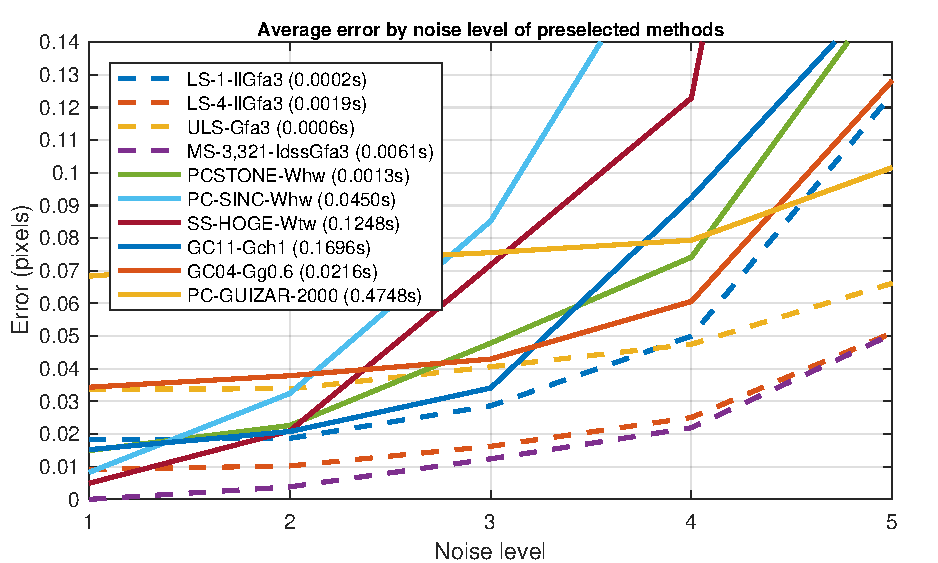
\includegraphics[width=\textwidth]{img/GroupedTop10ByNoise}
\caption{Top ten methods by noise level}
\end{subfigure}%
\begin{subfigure}{.5\textwidth}
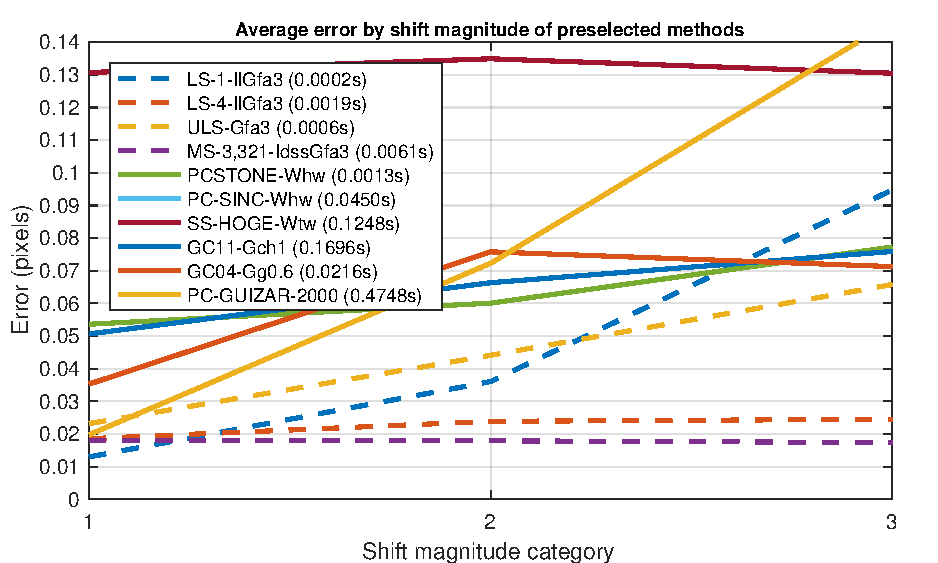
\includegraphics[width=\textwidth]{img/groupedTop10ByShift}
\caption{Top ten methods by shift magnitude category}
\end{subfigure}
\caption{Average error for some variants of preselected methods. \textbf{Left}: varying noise averaging over all shift magnitudes. \textbf{Right}: varying shift magnitude averaging over all noise levels.}
\label{fig:preselectedFigShiftEstimation}
\end{figure}

\subsubsection{A short study on multiscale gradient-based shift estimation}
\label{sec:iterativeVsMultiscaleGBSE}
We studied whether it is more convenient to iterate the standard GBSE approach in a direct fashion, i.e. using only one scale, or in a multiscale approach. To this end, both methodologies described in section \ref{sec:iterativeAndMultiScale} were evaluated under different noise conditions, shifts and gradient estimators. To show the most representative results, four SNR conditions were considered: noiseless, low noise ($\sigma=75$), medium noise ($\sigma=150$) and high noise ($\sigma=300$). Noise values are according to 12 bit images. Each table is organized in groups of four lines corresponding to each of these four noise configurations. Also, the four most significative shifts in terms of results are shown: a big shift $(0.5, -0.9)$,  a medium shift $(0.2, -0.2)$, a small shift $(0.024, 0.052)$ and no shift. 

The performance of each algorithm under each condition was evaluated by simulation using the same setup employed throughout this section. 
%For each noise and shift, 100 experiments were averaged, and each experiment was performed by shifting the large image using Fourier interpolation and taking a $50 \times 50$ subimage from a random position away from the edges to avoid  ringing artifacts followed by adding white Gaussian noise and evaluating all the methods (Fig. \ref{fig:experiments}). 
The results shown contain only valid shift estimations.


%\begin{figure}
%	\centering
%	\includegraphics[width=.50\textwidth]{img/CannesMini}
%	\caption{Input image}
%	\label{fig:inputImage}
%\end{figure}
%\vspace{-0.3cm}
%\vspace{-0.6cm}	

%\begin{figure}[t]%[htpb!]
%	\centering
%	\subfloat{\includegraphics[trim = 25mm 0mm 25mm 0mm, clip, width=.23\hsize]{img/frameFirst}} 
%	\subfloat{\includegraphics[trim = 25mm 0mm 25mm 0mm, clip, width=.23\hsize]{img/frameLast}}\,\,\,
%	\subfloat{\includegraphics[trim = 25mm 0mm 25mm 0mm, clip, width=.23\hsize]{img/pertFirstIm}}
%	\subfloat{\includegraphics[trim = 25mm 0mm 25mm 0mm, clip, width=.23\hsize]{img/pertSecondIm}}
%	\caption{Two problems: a noisy and an almost unidimensional gradient situation}
%	\label{fig:experiments}
%\end{figure}
%\vspace{-1cm}
\begin{table}[h!]%[htpb!] 
	\centering
	\begin{tabular}{c |l||c|c|c|c|c|c}
		\scriptsize{\textbf{Shift (px)}} & \scriptsize{\textbf{Noise}} & \scriptsize{\textbf{IT2Gh}} & \scriptsize{\textbf{IT2Gg1}} & \scriptsize{\textbf{IT2Gg0.3}} & \scriptsize{\textbf{MS2Gh}} & \scriptsize{\textbf{MS2Gg1}} & \scriptsize{\textbf{MS2Gg0.3}}\\ \hline 
\multirow{4}{*}{(0.5000,-0.9000)} & $\sigma=0$ & 0.0514 & 0.0818 & 0.0472 & 0.0387 & 0.1600 & \textbf{0.0316} \\ 
 & $\sigma=75$ & 0.1375 & 0.1053 & 0.1103 & 0.0744 & 0.1808 & \textbf{0.0582} \\ 
 & $\sigma=150$ & 0.2875 & 0.1414 & 0.2305 & 0.1267 & 0.2130 & \textbf{0.1009} \\ 
 & $\sigma=300$ & 0.4927 & 0.2327 & 0.4292 & 0.2319 & 0.2872 & \textbf{0.1909} \\ 
 \hline
\multirow{4}{*}{(0.0000,0.0000)} & $\sigma=0$ & \textbf{0.0000} & 0.0000 & 0.0000 & 0.0000 & 0.0000 & 0.0000 \\ 
 & $\sigma=75$ & \textbf{0.0114} & 0.0188 & 0.0132 & 0.0164 & 0.0188 & 0.0175 \\ 
 & $\sigma=150$ & \textbf{0.0168} & 0.0330 & 0.0219 & 0.0300 & 0.0326 & 0.0313 \\ 
 & $\sigma=300$ & \textbf{0.0191} & 0.0539 & 0.0307 & 0.0527 & 0.0549 & 0.0573 \\ 
 \hline
\multirow{4}{*}{(0.2000,-0.2000)} & $\sigma=0$ & 0.0115 & 0.0117 & 0.0154 & \textbf{0.0115} & 0.0360 & 0.0159 \\ 
 & $\sigma=75$ & 0.0249 & 0.0267 & 0.0223 & \textbf{0.0192} & 0.0470 & 0.0225 \\ 
 & $\sigma=150$ & 0.0652 & 0.0424 & 0.0487 & 0.0360 & 0.0591 & \textbf{0.0358} \\ 
 & $\sigma=300$ & 0.1295 & 0.0765 & 0.1103 & 0.0738 & 0.0899 & \textbf{0.0694} \\ 
 \hline
\multirow{4}{*}{(0.0240,0.0520)} & $\sigma=0$ & 0.0040 & \textbf{0.0019} & 0.0052 & 0.0039 & 0.0073 & 0.0054 \\ 
 & $\sigma=75$ & \textbf{0.0122} & 0.0181 & 0.0138 & 0.0156 & 0.0189 & 0.0166 \\ 
 & $\sigma=150$ & \textbf{0.0198} & 0.0326 & 0.0231 & 0.0296 & 0.0326 & 0.0311 \\ 
 & $\sigma=300$ & \textbf{0.0300} & 0.0543 & 0.0354 & 0.0547 & 0.0564 & 0.0581 \\ 
 \hline
\hline
\multirow{4}{*}{Avg.} & $\sigma=0$ & 0.0167 & 0.0238 & 0.0170 & 0.0135 & 0.0508 & \textbf{0.0132} \\ 
 & $\sigma=75$ & 0.0465 & 0.0422 & 0.0399 & 0.0314 & 0.0664 & \textbf{0.0287} \\ 
 & $\sigma=150$ & 0.0973 & 0.0624 & 0.0811 & 0.0556 & 0.0843 & \textbf{0.0498} \\ 
 & $\sigma=300$ & 0.1678 & 0.1043 & 0.1514 & 0.1033 & 0.1221 & \textbf{0.0939} \\ 
\hline
\end{tabular}
	\caption{\small{Estimation error (in pixels) per shift of every method using \textbf{two iterations} and \textbf{bicubic} interpolation from valid estimations. For each shift and estimation method, four SNR conditions were tested. The first three columns are for the iterative method (IT) while the last three are for the multiscale approach (MS) with a single iteration per scale. In each case, three gradient estimation methods were used: backward difference and Gaussian derivative with $\sigma=1$ and with $\sigma=0.3$ respectively.}}
	\label{tab:table1}
\end{table}
%\vspace{-0.7cm}
\begin{table}[t]%[t!]
\small
\centering
\begin{tabular}{c|l||c|c|c|c|c|c}
\scriptsize{\textbf{Shift (px)}} & \scriptsize{\textbf{Noise}} & \scriptsize{\textbf{IT3Gh}} & \scriptsize{\textbf{IT3Gg1}} & \scriptsize{\textbf{IT3Gg0.3}} & \scriptsize{\textbf{MS3Gh}} & \scriptsize{\textbf{MS3Gg1}} & \scriptsize{\textbf{MS3Gg0.3}}\\ \hline 
\multirow{4}{*}{(0.5000,-0.9000)} & $\sigma=0$ & 0.0156 & 0.0238 & \textbf{0.0065} & 0.0114 & 0.1007 & 0.0086 \\ 
 & $\sigma=75$ & 0.0646 & 0.0437 & 0.0437 & 0.0293 & 0.1194 & \textbf{0.0251} \\ 
 & $\sigma=150$ & 0.1869 & 0.0727 & 0.1326 & 0.0533 & 0.1488 & \textbf{0.0497} \\ 
 & $\sigma=300$ & 0.4092 & 0.1480 & 0.3337 & 0.1093 & 0.2143 & \textbf{0.1001} \\ 
 \hline
\multirow{4}{*}{(0.0000,0.0000)} & $\sigma=0$ & \textbf{0.0000} & 0.0000 & 0.0000 & 0.0000 & 0.0000 & 0.0000 \\ 
 & $\sigma=75$ & \textbf{0.0116} & 0.0199 & 0.0133 & 0.0261 & 0.0330 & 0.0260 \\ 
 & $\sigma=150$ & \textbf{0.0194} & 0.0357 & 0.0246 & 0.0468 & 0.0547 & 0.0467 \\ 
 & $\sigma=300$ & \textbf{0.0250} & 0.0621 & 0.0391 & 0.0980 & 0.1065 & 0.1001 \\ 
 \hline
\multirow{4}{*}{(0.2000,-0.2000)} & $\sigma=0$ & \textbf{0.0027} & 0.0045 & 0.0043 & 0.0206 & 0.0205 & 0.0235 \\ 
 & $\sigma=75$ & 0.0201 & 0.0229 & \textbf{0.0182} & 0.0304 & 0.0430 & 0.0334 \\ 
 & $\sigma=150$ & 0.0475 & 0.0395 & \textbf{0.0373} & 0.0483 & 0.0593 & 0.0489 \\ 
 & $\sigma=300$ & 0.1096 & \textbf{0.0718} & 0.0913 & 0.0982 & 0.1195 & 0.0977 \\ 
 \hline
\multirow{4}{*}{(0.0240,0.0520)} & $\sigma=0$ & \textbf{0.0007} & 0.0009 & 0.0013 & 0.0068 & 0.0041 & 0.0080 \\ 
 & $\sigma=75$ & \textbf{0.0120} & 0.0188 & 0.0132 & 0.0219 & 0.0283 & 0.0225 \\ 
 & $\sigma=150$ & \textbf{0.0207} & 0.0348 & 0.0248 & 0.0471 & 0.0548 & 0.0464 \\ 
 & $\sigma=300$ & \textbf{0.0313} & 0.0622 & 0.0412 & 0.1011 & 0.1056 & 0.1001 \\ 
 \hline
\hline
\multirow{4}{*}{Avg.} & $\sigma=0$ & 0.0047 & 0.0073 & \textbf{0.0030} & 0.0097 & 0.0313 & 0.0100 \\ 
 & $\sigma=75$ & 0.0271 & 0.0263 & \textbf{0.0221} & 0.0269 & 0.0559 & 0.0268 \\ 
 & $\sigma=150$ & 0.0686 & \textbf{0.0457} & 0.0548 & 0.0489 & 0.0794 & 0.0479 \\ 
 & $\sigma=300$ & 0.1438 & \textbf{0.0860} & 0.1263 & 0.1017 & 0.1365 & 0.0995 \\ 
\hline
\end{tabular}
	\caption{\small{Estimation error (in pixels) per shift of every method using \textbf{three iterations} and \textbf{spline} interpolation from valid estimations. Table configuration is the same as in Table \ref{tab:table1}.}}
	\label{tab:table2}
\end{table}

%
In tables \ref{tab:table1} and \ref{tab:table2} results are shown for two iterations and bicubic interpolation, and for three iterations with spline interpolation respectively. %The first three colums stand for the iterative method, using a backward difference derivative, a Gaussian derivative with $\sigma=1$ and a Gaussian derivative with $\sigma=0.3$. The last three columns is the multiscale method with only one iteration between scales using the same three derivatives.
%
From these results several conclusions can be drawn.
\begin{itemize}
\item First, as expected, the multiscale method is much more robust when the shift magnitude is high. In fact, even at a shift as low as (0.2,-0.2) it is recommendable to use the multiscale method instead of the standard iterative version. 
\item Second, when no shift or  a small shift is present, the single-scale methods achieve much better accuracies. Apparently, the multiscale algorithms are not suited for such small shifts since their poor performance on lower scales results in less accurate results. This result contradicts several state-of-the-art methods and is worth remarking. 
\item Third, regarding the amount of iterations/scales to use, in presence of high noise, performing more iterations in the original scale or using more scales in the multiscale approach gives worse results in terms of accuracy. When dealing with a noisy situation, the resampling operation proved to be negative for the shift estimation algorithm. This result is more accentuated for the multiscale approach.
\item Finally, the multiscale algorithm proved to be a better contender when dealing with noise in general, although this factor is greatly influenced by the shift magnitude. However, except when the shift magnitude is lower than a fifth of a pixel, its use is recommended. Moreover, its computational cost is lower than the iterative counterpart since the resampling is performed on lower resolution images.
\end{itemize}


\subsubsection{Conclusions}
\label{sec:summaryShiftEstimationUnderNoise}
To summarize, the conclusions for this section are:
\begin{itemize}
\setlength\itemsep{-0.5em}
\item The \magnify{best overall method} proved to be the \magnify{multiscale GBSE} approach using three scales. The best iteration/resampling configuration on the scales was to do a single iteration on the coarsest scale, followed by performing two iterations in the middle scale using spline interpolation, and applying three iterations on the finest (original) scale using FFT with symmetrization as the interpolation method. 
\item The best method type in general is gradient-based, and \magnify{the amount of iterations and/or scales depends on the shift magnitude to estimate}.
\item The \magnify{derivative} for GBSE methods that proved to be the \magnify{most robust to noise} was the one proposed by \magnify{Farid \cite{farid2004differentiation} using a $3 \times 3$ support}, although the $3 \times 3$ variant of the Simoncelli derivative \cite{Simoncelli_1994} achieved similar results.
\item For \magnify{low shift magnitudes} (category 1 in Table \ref{tab:shiftMagnitudeCategories}) the best methods are again gradient-based and the recommended gradient estimation method to use was the \magnify{hypomode}.
\item For \magnify{shift magnitudes larger than 0.5}, a \magnify{multiscale approach} is mandatory.
\item \magnify{Phase correlation methods suffer from low SNR scenarios}.
\item In general, \magnify{gradient correlation-based methods improve over phase correlation methods}, and this difference becomes more important as the noise increases.
\item For phase-correlation-based methods, the \magnify{best windows} used for apodization proved to be the \magnify{Hamming} window, the \magnify{Blackman} window and the \magnify{Tukey} window. Also, in several cases, \magnify{avoiding apodization} yielded the best results.
\item The TLS GBSE method proved in general to be more accurate than both the standard LS and the CLS variant. For the TLS approach, a singular value decomposition is required, which may be expensive in some cases. In contrast, the CLS method requires the knowledge of the noise standard deviation, which may not be available in some situations. \magnify{If the TLS} method is used, \magnify{validating} using existing approaches \cite{Weber95robustcomputation, Tsai1998} \magnify{must be done} since it proved to be unstable on many situations, particularly under lower SNRs.
\item On shifts with \magnify{magnitudes between 0.1 and 1.1}, the \magnify{bidirectional bias corrected method} of Pham \emph{et al.} \cite{pham2008} achieves good results without requiring interpolation nor an iterative procedure, thus singling it out as the \magnify{best overall low-cost method}. As an exception, if the shift magnitude is \emph{a-priori} known to be lower than 0.1, a single iteration of the total least squares method gets the best results among the fast methods.
\item For \magnify{large shift magnitudes} (last category in Table \ref{tab:shiftMagnitudeCategories}), the \magnify{multiscale GBSE} method always achieved the best results. However, it should be noted that the amount of scales used depends on the maximum possible shift magnitude to estimate. Since in the evaluated setup, the maximum displacement was known \emph{a-priori}, the amount of scales was set according to it. If however this information is not known, phase/gradient correlation-based methods should be used. In particular, for high SNR scenarios, either fitting a sinc on the PCS \cite{Foroosh2002} or using Hoge's subspace method \cite{Hoge_2003} yielded the best results. Under \magnify{lower SNR}, \magnify{gradient correlation} approaches should be employed.
\end{itemize}

\subsection{Robustness to violation of the brightness constancy constraint}
While GBSE methods rely on the brightness constancy constraint, the main strength of phase-correlation methods is their higher tolerance against image changes. Therefore, we performed an experiment, using the same setup described in this section,  where a square of size $K \times K$ was removed (i.e., set to white) from the center of the first image before estimating the shift. We tested with $K = [3, 5, 7, 9, 11]$, which, given that the shift is estimated using $50 \times 50$ images, this implies removing up to $5\%$ of the image. The results of this are displayed in Fig.~\ref{fig:occlusion} for the five values of $K$. All methods were evaluated using two noise levels: low noise ($\sigma = 0.005$) or high noise ($\sigma = 0.055$).

\begin{figure}[H]
	\centering
	\begin{subfigure}{.15\linewidth}
		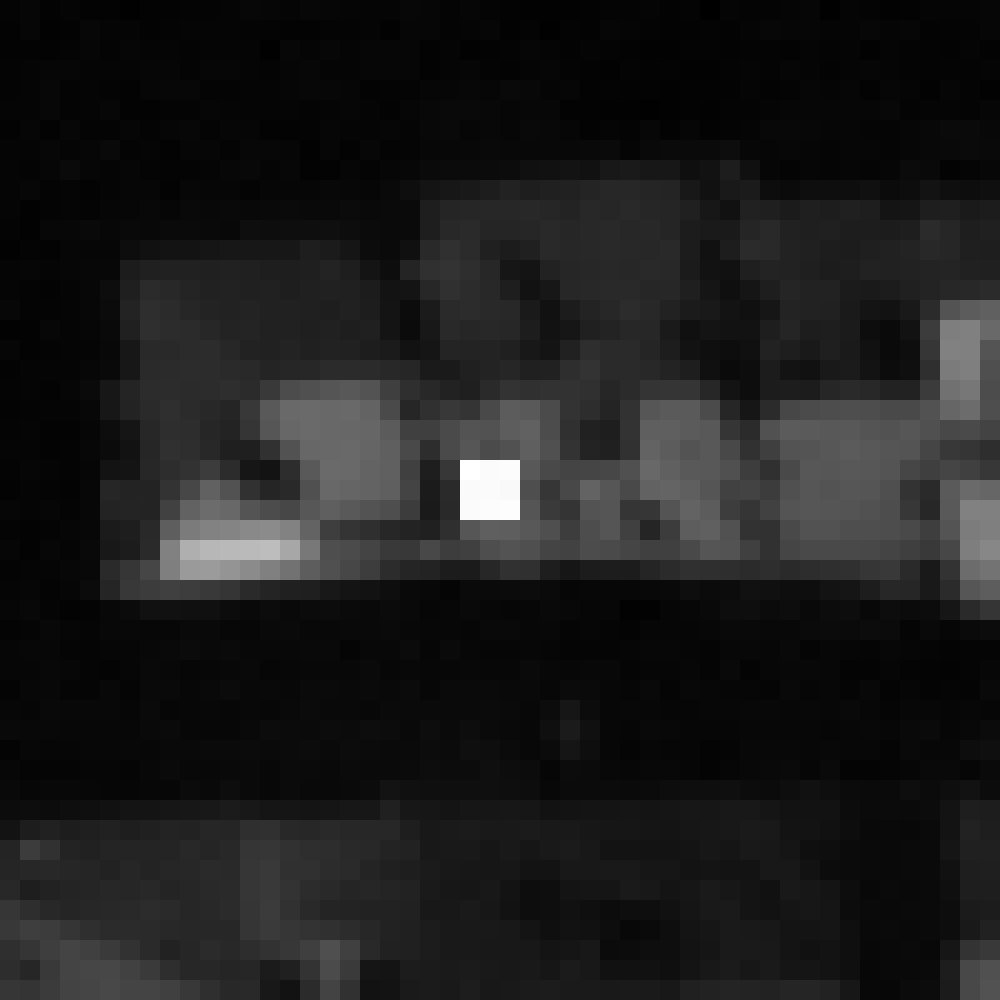
\includegraphics[width=1\textwidth]{img/testOcclusion1}
		\caption{{$K=3$}}
	\end{subfigure}
	\begin{subfigure}{.15\linewidth}
		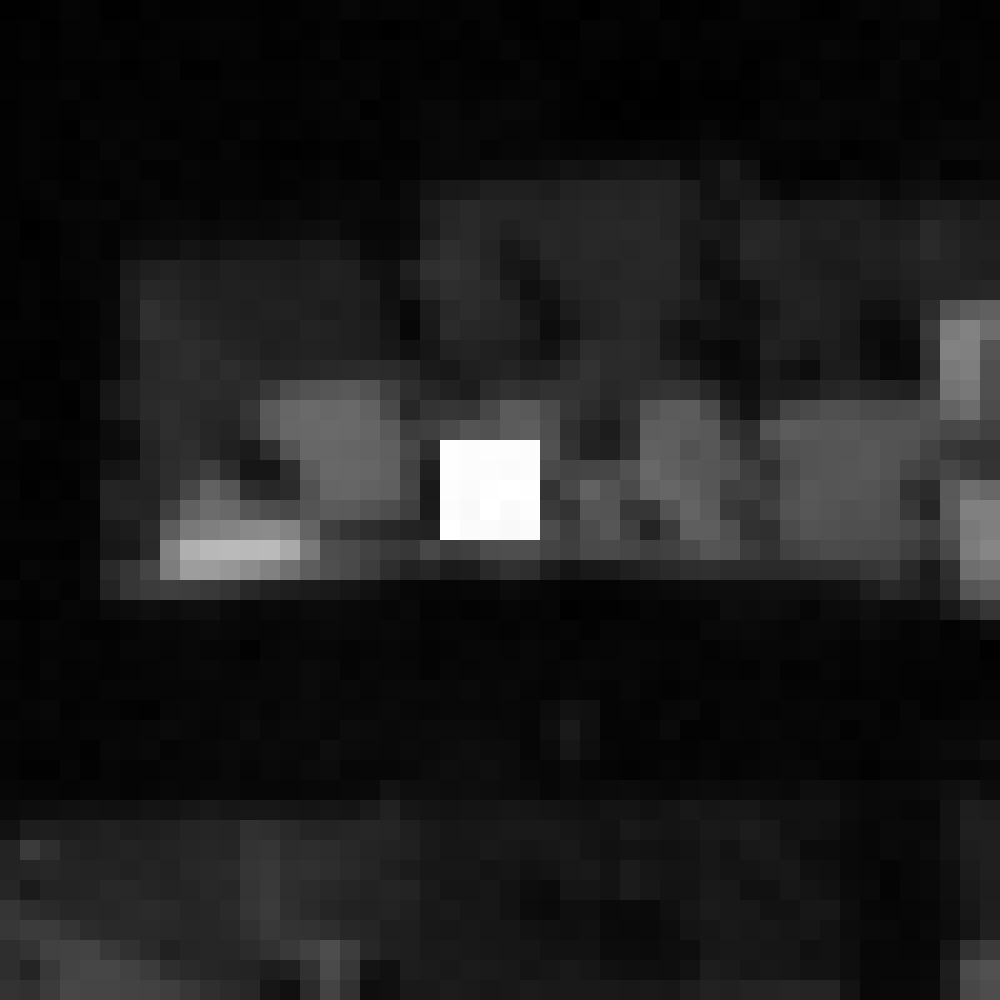
\includegraphics[width=1\textwidth]{img/testOcclusion2}
		\caption{{$K=5$}}
	\end{subfigure} 
	\begin{subfigure}{.15\linewidth}
		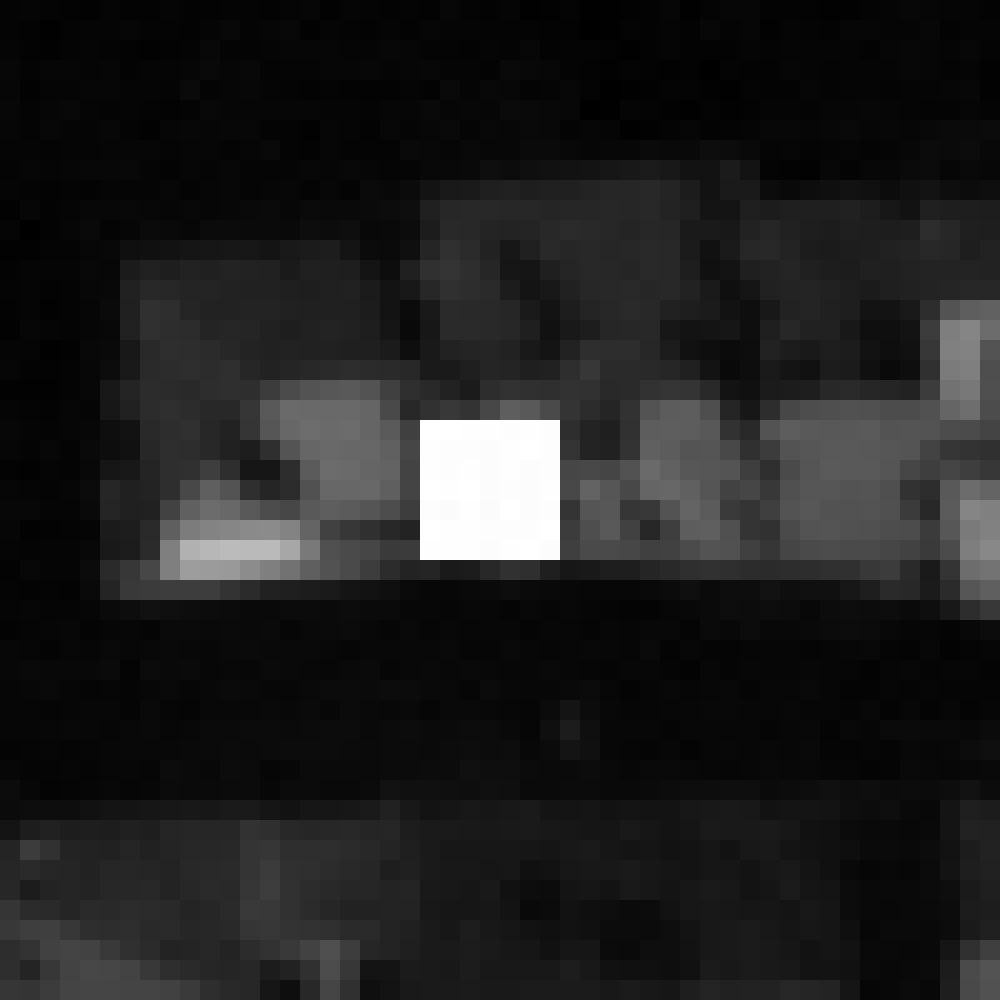
\includegraphics[width=1\textwidth]{img/testOcclusion3}
		\caption{{$K=7$}}
	\end{subfigure}
	\begin{subfigure}{.15\linewidth}
		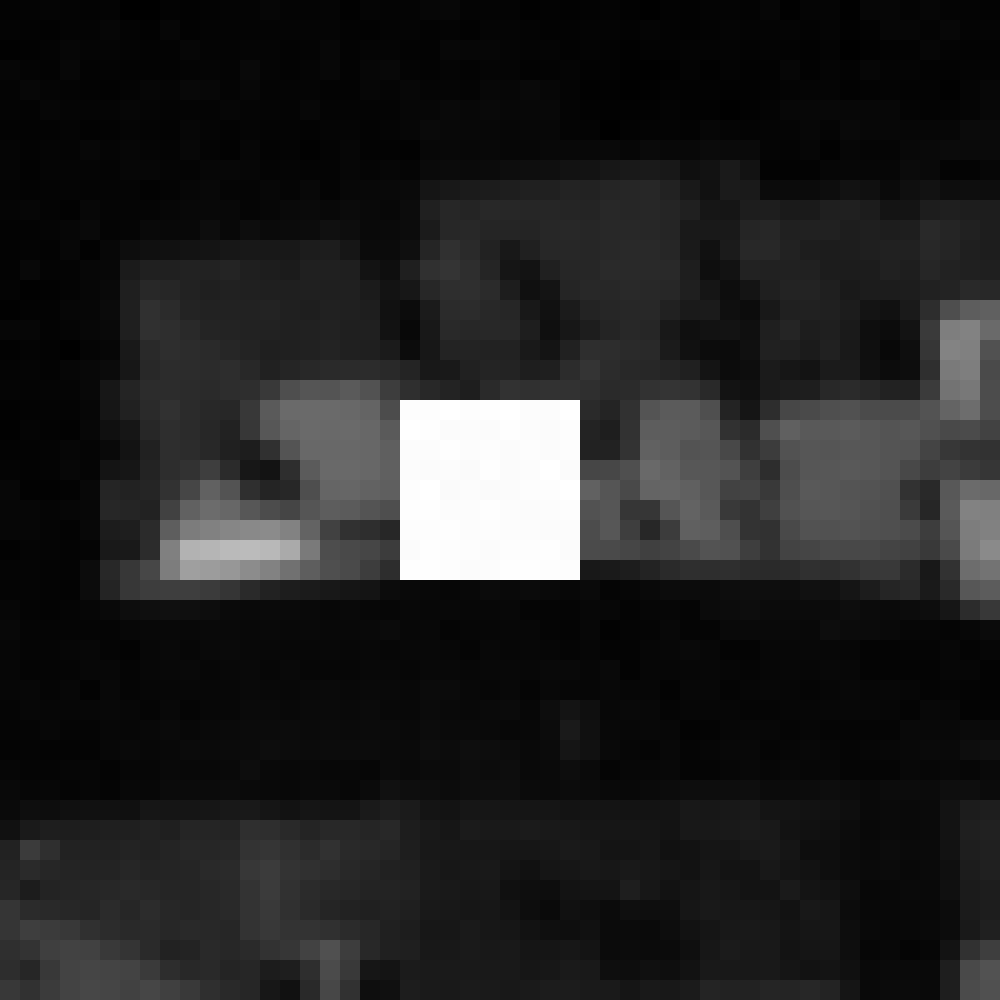
\includegraphics[width=1\textwidth]{img/testOcclusion4}
		\caption{{$K=9$}}
	\end{subfigure}
	\begin{subfigure}{.15\linewidth}
		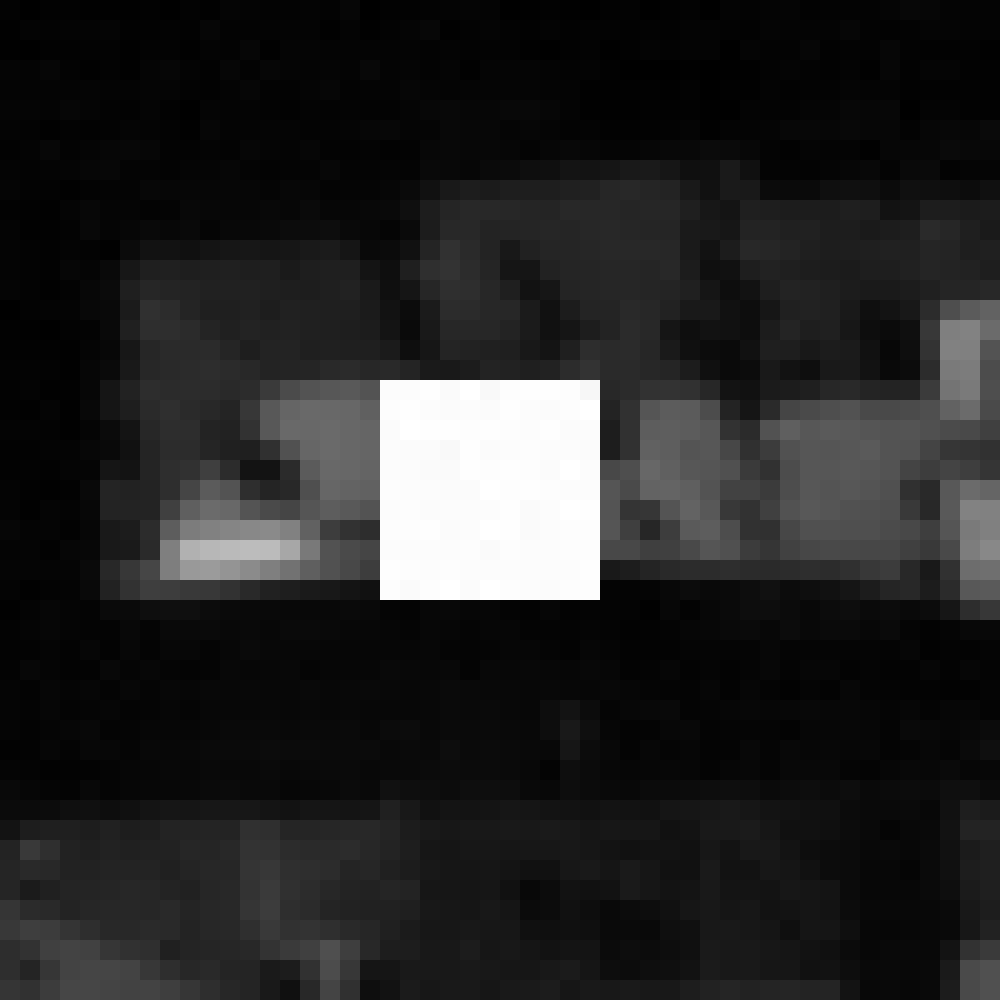
\includegraphics[width=1\textwidth]{img/testOcclusion5}
		\caption{$K=11$}
	\end{subfigure}%		
	\caption{Example evaluated subimages for the five different values of $K$.}
	\label{fig:occlusion}
\end{figure}

In Table \ref{tab:occlusion1} we observe the top 5 methods averaged over shift magnitudes one to three. Although a decrease in performance is observed for GBSE methods, they still improve over phase correlation methods under shift magnitudes lower than one pixel. However, when evaluating shift magnitudes higher than one pixel (category four from Table \ref{tab:shiftMagnitudeCategories}), the situation is different, as seen from Table \ref{tab:occlusion2}. In fact, GBSE methods still achieve the best accuracies when the size of the removed square is $K=3$ or, in case of high noise, when $K \leq 7$. On every other case, GBSE methods are not recommended. For example, with $K=11$, the best results were obtained using phase correlation methods as expected, and most importantly, under high SNR scenarios, the difference between them and the best performing GBSE variant was up to four times better in terms of the measured error in pixels. What is worse, since the deleted square was removed from the center of each subimage, then the windowing procedure applied before computing the phase correlation removes almost all the image information (this explains why the best performing PC methods did not perform apodization). Since the difference between both images does not necessarily have to be in the center, this implies phase correlation-based methods should obtain even better results accentuating the improvement with respect to GBSE methods. 

\begin{table}[ht!]
\scriptsize
\setlength{\tabcolsep}{1pt}
\renewcommand{\arraystretch}{1}
%\hspace{-7mm}
\begin{tabular}{|c|l|l|l|l|l|}\hline
& \multicolumn{1}{|c|}{$K=3$} & \multicolumn{1}{|c|}{$K=5$} & \multicolumn{1}{|c|}{$K=7$} & \multicolumn{1}{|c|}{$K=9$} & \multicolumn{1}{|c|}{$K=11$} \\ \hline 
\begin{tabular}{c}$\sigma$\\$0.005$\end{tabular} & \begin{tabular}{l}0.0231\ MS-3,321-IfssGh\\0.0234\ LS-4-IdGch2\\0.0241\ TLS-4-IdGg0.3\\0.0279\ CLS-4-IfGg0.6\\0.0565\ ADF2-2QI\\\end{tabular} & 
\begin{tabular}{l}0.0376\ LS-4-IfGch2\\0.0376\ MS-2-LS4-IfGch2\\0.0428\ TLS-4-IdGch1\\0.0505\ CLS-4-IfGg0.6\\0.0730\ ULS-Gch1\\\end{tabular} & 
\begin{tabular}{l}0.0632\ LS-4-IfGch2\\0.0632\ MS-2-LS4-IfGch2\\0.0739\ CLS-4-IdGch1\\0.0766\ TLS-4-IdGch1\\0.0991\ PC-SINC-Wnw\\\end{tabular} & 
\begin{tabular}{l}0.0762\ LS-4-IfGch2\\0.0762\ MS-2-LS4-IfGch2\\0.0883\ CLS-4-IdGch1\\0.0967\ PC-SINC-Wnw\\0.1196\ ULS-Gh\\\end{tabular} & 
\begin{tabular}{l}0.0940\ PC-SINC-Wnw\\0.0944\ LS-4-IfGch2\\0.0944\ MS-2-LS4-IfGch2\\0.1474\ CLS-4-IfGfa3\\0.1506\ PCSTONE-Wnw\\\end{tabular} 
\\ \hline
\begin{tabular}{c}$\sigma$\\$0.055$\end{tabular} & \begin{tabular}{l}0.0645\ MS-2,31-IscGfa3\\0.0664\ CLS-4-IfGg0.6\\0.0665\ LS-4-IdGfa3\\0.0796\ TLS-4-IfGh\\0.0933\ ULS-Gh\\\end{tabular} & 
\begin{tabular}{l}0.0815\ CLS-4-IdGg0.6\\0.0831\ LS-4-IdGfa3\\0.0831\ MS-2-LS4-IdGfa3\\0.1117\ TLS-4-IdGh\\0.1207\ ULS-Gch2\\\end{tabular} & 
\begin{tabular}{l}0.1016\ LS-4-IfGfa3\\0.1016\ MS-2-LS4-IfGfa3\\0.1030\ CLS-4-IfGg0.6\\0.1221\ ULS-Gh\\0.1460\ TLS-4-IdGh\\\end{tabular} & 
\begin{tabular}{l}0.1221\ LS-4-IfGfa3\\0.1221\ MS-2-LS4-IfGfa3\\0.1380\ CLS-4-IfGfa3\\0.1559\ PCSTONE-Wnw\\0.1622\ ULS-Gg0.3\\\end{tabular} & 
\begin{tabular}{l}0.1486\ LS-4-IfGch2\\0.1486\ MS-2-LS4-IfGch2\\0.1546\ CLS-4-IdGch1\\0.1651\ PCSTONE-Wnw\\0.1814\ TLS-4-IcGch1\\\end{tabular} 
\\ \hline
\end{tabular}
\caption{Average error of top 5 evaluated methods per noise and $K$ value for shift magnitudes one to three. \textbf{Rows}: two noise levels. \textbf{Columns}: five $K$ values. Only the best variant per method is displayed.}
\label{tab:occlusion1}
\end{table}

\begin{table}[ht!]
\scriptsize
\setlength{\tabcolsep}{1pt}
\renewcommand{\arraystretch}{1}
\hspace{-7mm}
\begin{tabular}{|c|l|l|l|l|l|}\hline
& \multicolumn{1}{|c|}{$K=3$} & \multicolumn{1}{|c|}{$K=5$} & \multicolumn{1}{|c|}{$K=7$} & \multicolumn{1}{|c|}{$K=9$} & \multicolumn{1}{|c|}{$K=11$} \\ \hline 
\begin{tabular}{c}$\sigma$\\$0.005$\end{tabular} & \begin{tabular}{l}0.0324\ MS-4,4321-IfssssGh\\0.0484\ ADF2-2QI\\0.0874\ ADF-2QI\\0.1286\ GC04-Gch3\\0.1935\ GC11-Gg0.3\\0.2012\ PCSINC-Wnw\\0.2098\ PCESINC-Wnw\\\end{tabular} & 
\begin{tabular}{l}0.0525\ ADF2-2QI\\0.0781\ MS-5,54321-IfssssGch1\\0.0868\ ADF-2QI\\0.1274\ PCSINC-Wnw\\0.1359\ PCESINC-Wnw\\0.1461\ PCREN2010-Wnw\\0.3391\ SS-HOGE-Wnw\\\end{tabular} & 
\begin{tabular}{l}0.1121\ PCSINC-Wnw\\0.1190\ PCESINC-Wnw\\0.1284\ PCREN2010-Wnw\\0.2022\ MS-4,4321-IfssssGh\\0.3194\ PCQUADFIT\\0.4191\ SS-HOGE-Wnw\\0.4525\ PCGAUSSFIT\\\end{tabular} & 
\begin{tabular}{l}0.1511\ PCSINC-Wnw\\0.1593\ PCESINC-Wnw\\0.1669\ PCREN2010-Wnw\\0.3735\ PCQUADFIT\\0.4677\ MS-3,321-IsssGfa3\\0.5036\ PCGAUSSFIT\\0.5449\ SS-HOGE-Wnw\\\end{tabular} & 
\begin{tabular}{l}0.1888\ PCSINC-Wnw\\0.1935\ PCESINC-Wnw\\0.2018\ PCREN2010-Wnw\\0.5107\ PCQUADFIT\\0.6405\ PCGAUSSFIT\\0.7407\ SS-HOGE-Wnw\\0.7662\ MS-3,321-IsssGfa3\\\end{tabular} 
\\ \hline
\begin{tabular}{c}$\sigma$\\$0.055$\end{tabular} & \begin{tabular}{l}0.1434\ MS-4,4321-IsssssGh\\0.4550\ PCREN2010-Wnw\\0.4589\ PCESINC-Wnw\\0.4649\ PCSINC-Wnw\\0.6876\ GC04-Gch3\\0.7474\ PCQUADFIT\\0.8013\ PCGAUSSFIT\\\end{tabular} & 
\begin{tabular}{l}0.1512\ MS-5,54321-IsssssGch1\\0.4168\ PCESINC-Wnw\\0.4176\ PCREN2010-Wnw\\0.4228\ PCSINC-Wnw\\0.6585\ PCQUADFIT\\0.6693\ GC04-G5\\0.7211\ PCGAUSSFIT\\\end{tabular} & 
\begin{tabular}{l}0.4121\ MS-3,321-IsssGfa3\\0.5034\ PCREN2010-Wnw\\0.5051\ PCESINC-Wnw\\0.5117\ PCSINC-Wnw\\0.7304\ PCQUADFIT\\0.7952\ PCGAUSSFIT\\0.9658\ PCFOO\\\end{tabular} & 
\begin{tabular}{l}0.6444\ PCESINC-Wnw\\0.6476\ PCREN2010-Wnw\\0.6496\ PCSINC-Wnw\\0.6640\ MS-3,321-IsssGfa3\\0.8098\ PCQUADFIT\\0.8154\ GC11-Gch2\\0.8858\ PCGAUSSFIT\\\end{tabular} & 
\begin{tabular}{l}0.6636\ PCESINC-Wex\\0.6654\ PCREN2010-Wex\\0.6717\ PCSINC-Wex\\0.7000\ PCQUADFIT\\0.7557\ PCGAUSSFIT\\0.7859\ MS-3,321-IsssGfa3\\0.9326\ PCFOO\\\end{tabular} 
\\ \hline
\end{tabular}
\caption{Average error of top 7 evaluated methods per noise and $K$ value for the fourth shift magnitude. \textbf{Rows}: two noise levels. \textbf{Columns}: five $K$ values. Only the best variant per method is displayed.}
\label{tab:occlusion2}
\end{table}

\subsubsection{Conclusions from these experiments}
\label{sec:occlusionsConclusionsChapter1}
In this section, we studied the behaviour of shift estimation methods when both images differ. This difference could be caused for example, by occlusions, different information appearing on each spectra on multi-spectral images or because both images were taken at different moments in time. In these cases, when the underlying displacement is lower than one pixel (categories one to three from Table \ref{tab:shiftMagnitudeCategories}), GBSE methods yield the best results. However, with larger displacement magnitudes, phase correlation approaches should be considered. In particular, with high SNR, phase correlation methods that use local function fitting in the spatial domain, described in section \ref{subsec:phaseCorrelationLocalFunctionFitting}, yield the best results and dramatically improve over GBSE methods. Under lower SNR scenarios, the improvement of PC over GBSE methods becomes less significative, and both approaches should be considered.

\subsection{Robustness to aliased sample processes}
We evaluated the robustness of each approach to aliasing. To simulate aliasing, we first applied a Gaussian low-pass filter of parameter $\sigma_A$ to a high-resolution image, yielding $\bar{I} = g_{\sigma_a} * I$ where $g$ denotes the Gaussian kernel and $*$ the convolution operator. Then we took both images
\begin{equation}
\tilde{I}_1	= subsample(\bar{I}) \quad \tilde{I}_2 = subsample(shift(\bar{I},d))
\end{equation}
where $shift$ is an integer resampling method (only moves the pixels), $d$ is 16 times the desired subpixel displacement and $subsample$ subsamples the image by regularly sampling 1 out of 16 pixels.
We evaluated $d = [-7, -4, 0, 8]\times [-7, -4, 0, 8]$, where in this case $\times$ corresponds to the cartesian product. In total, this implied estimating 16 subpixel shifts where for each dimension the shifts were $[-0.4375, -0.25, 0, 0.5]$. To test different levels of aliasing, we used five values for $\sigma_A$ displayed in Table \ref{tab:aliasingLevels}.
\begin{table}[htpb]
\centering
\begin{tabular}{|c|c|c|c|c|c|} 
	\hline
	Level & 1 & 2 & 3 & 4 & 5\\ \hline
	$\sigma_A$ & 8 & 6.4 & 4 & 2.8 & 0.8\\ \hline
\end{tabular}
\caption{Values of the standard deviation of the Gaussian used to prefilter the image before subsampling to generate different aliasing levels}
\label{tab:aliasingLevels}
\end{table}
%, namely $\sigma_A \in [8, 6.4, 4, 2.8, 0.8]$. 

%\nota{I would a table as I show the results. The top 10 and the top fast 10. Also, I would do a graph where I should in X the Aliasing level, in Y the error and show in it one (the best) method representative for each class. Perhaps another graph with is std. dev.}
All experiments were performed using the same two subimages extracted from the same location of both $\tilde{I}_1$ and $\tilde{I}_2$ respectively, by adding a mild noise of $\sigma_N=75$ which is equivalent to noise level 3. Both images are displayed in Fig.~\ref{fig:aliasedImages} for the five simulated levels of aliasing for the shift $(-0.25, 0.5)$ which proved to be troublesome for several methods. The difference between compensated images $\tilde{I}_1(x,y) - \tilde{I}_2(x+0.25, y-0.5)$, shown on the bottom row of the figure, illustrates the effects of aliasing on the shift estimation problem. As the aliasing level increases, more differences appear on the edges of the objects, and these differences gets larger in value. These differences may also disorient shift estimation methods generating non-existing secondary motions which alter the final results. 

\begin{figure}[t]
\centering
\begin{subfigure}{0.2\textwidth}
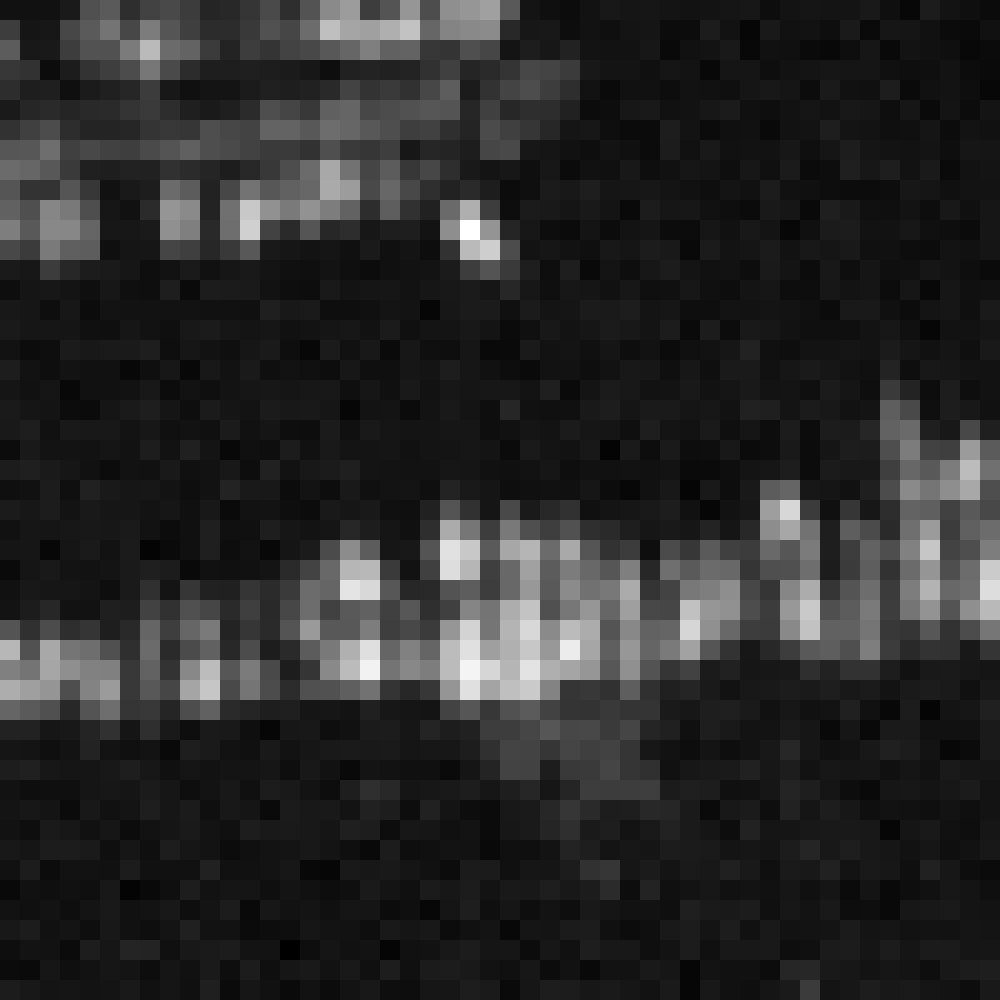
\includegraphics[width=\textwidth]{img/aliasedImg1L1}
\end{subfigure}%
\begin{subfigure}{0.2\textwidth}
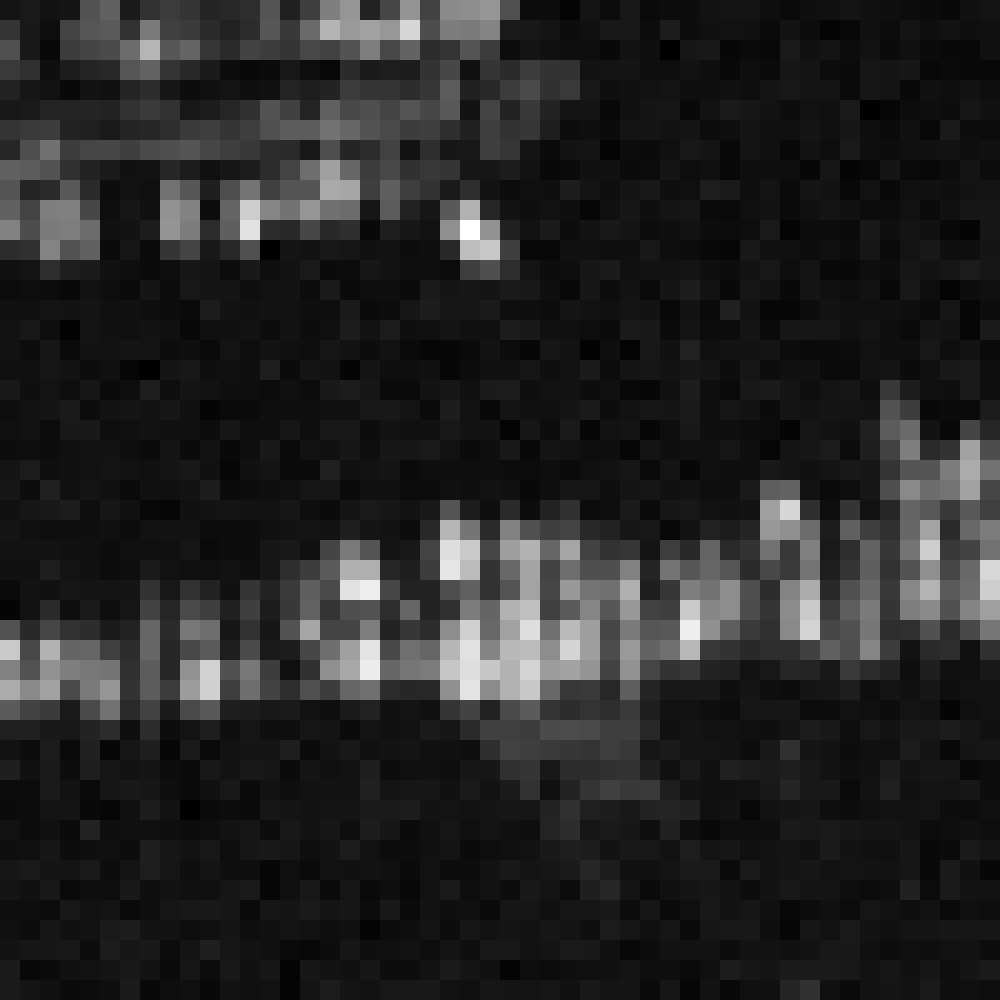
\includegraphics[width=\textwidth]{img/aliasedImg1L2}
\end{subfigure}%
\begin{subfigure}{0.2\textwidth}
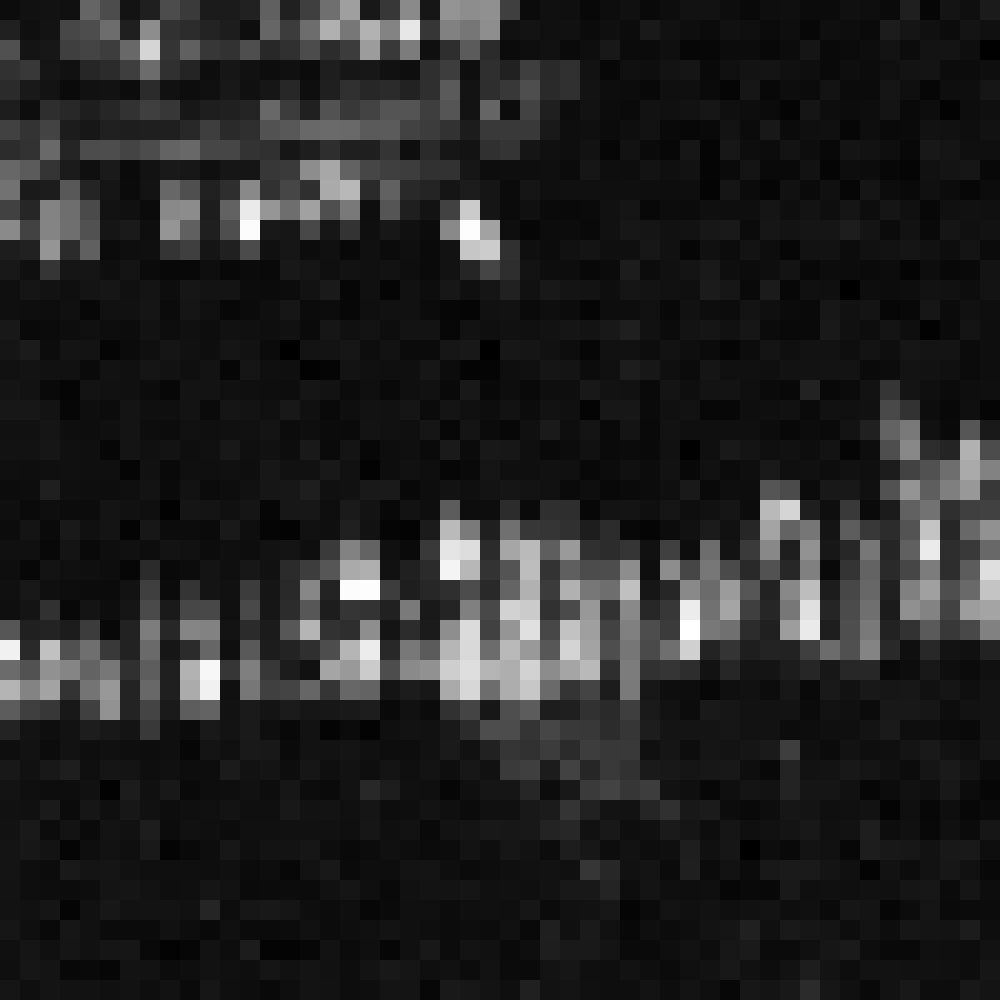
\includegraphics[width=\textwidth]{img/aliasedImg1L3}
\end{subfigure}%
\begin{subfigure}{0.2\textwidth}
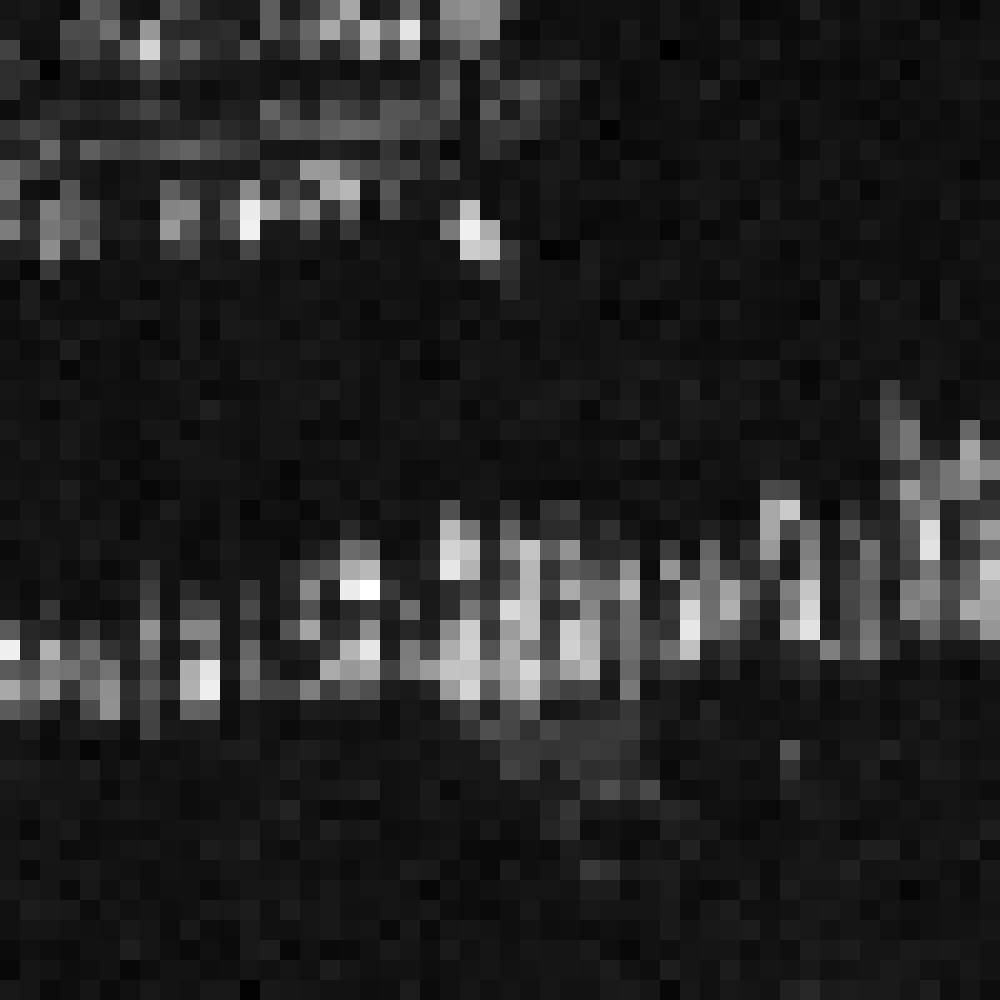
\includegraphics[width=\textwidth]{img/aliasedImg1L4}
\end{subfigure}%
\begin{subfigure}{0.2\textwidth}
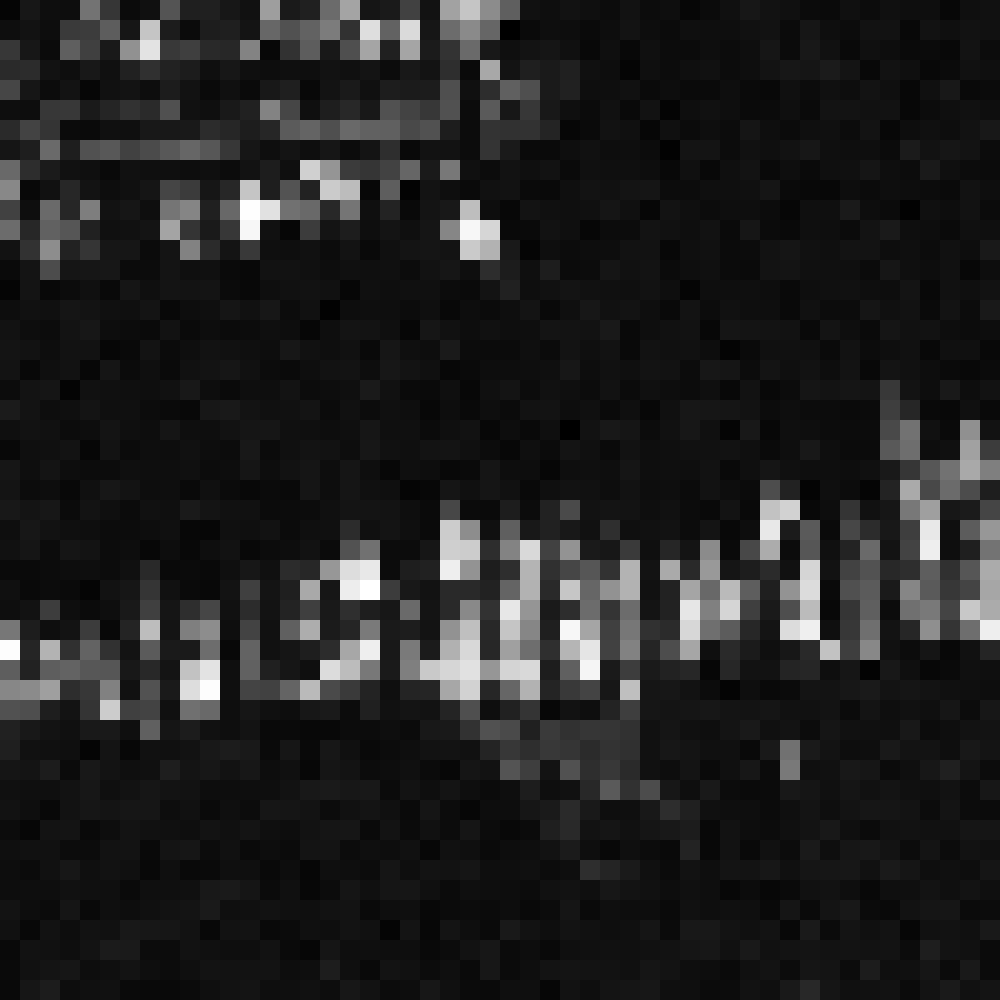
\includegraphics[width=\textwidth]{img/aliasedImg1L5}
\end{subfigure}
\begin{subfigure}{0.2\textwidth}
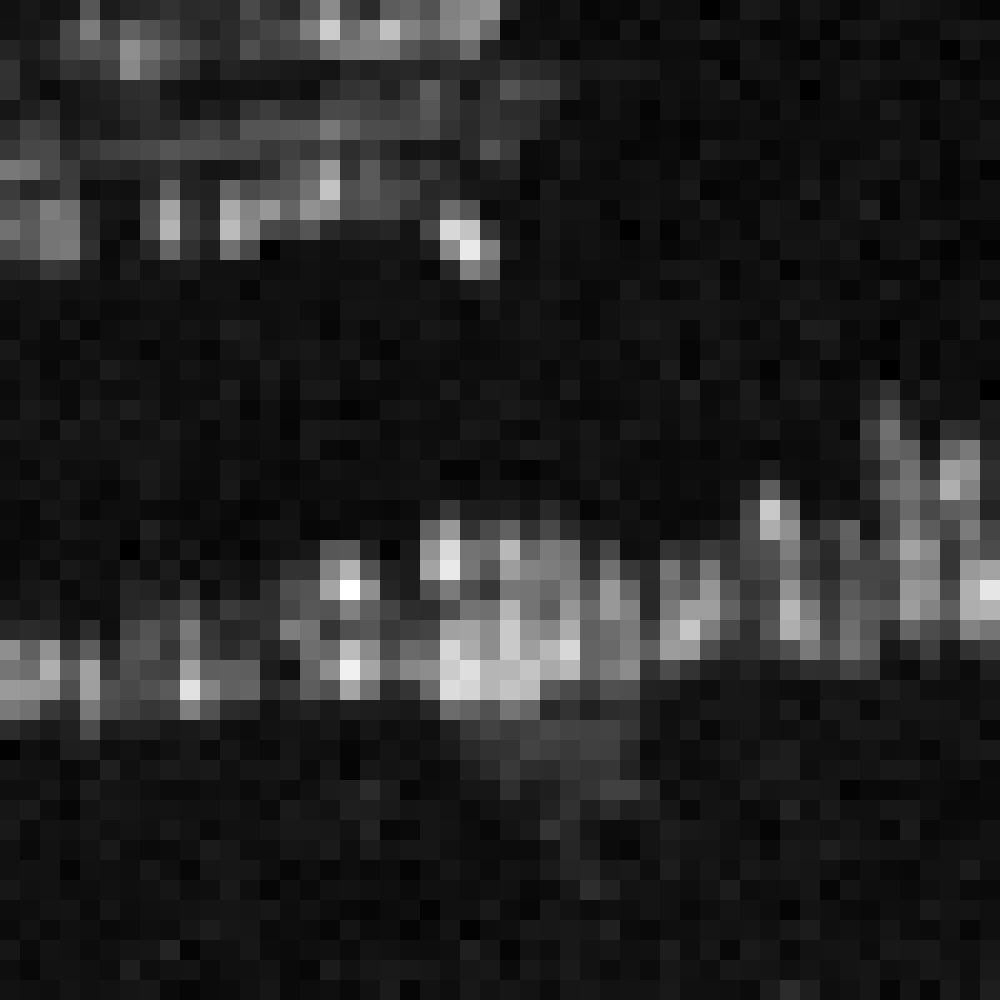
\includegraphics[width=\textwidth]{img/aliasedImg2L1}
\end{subfigure}%
\begin{subfigure}{0.2\textwidth}
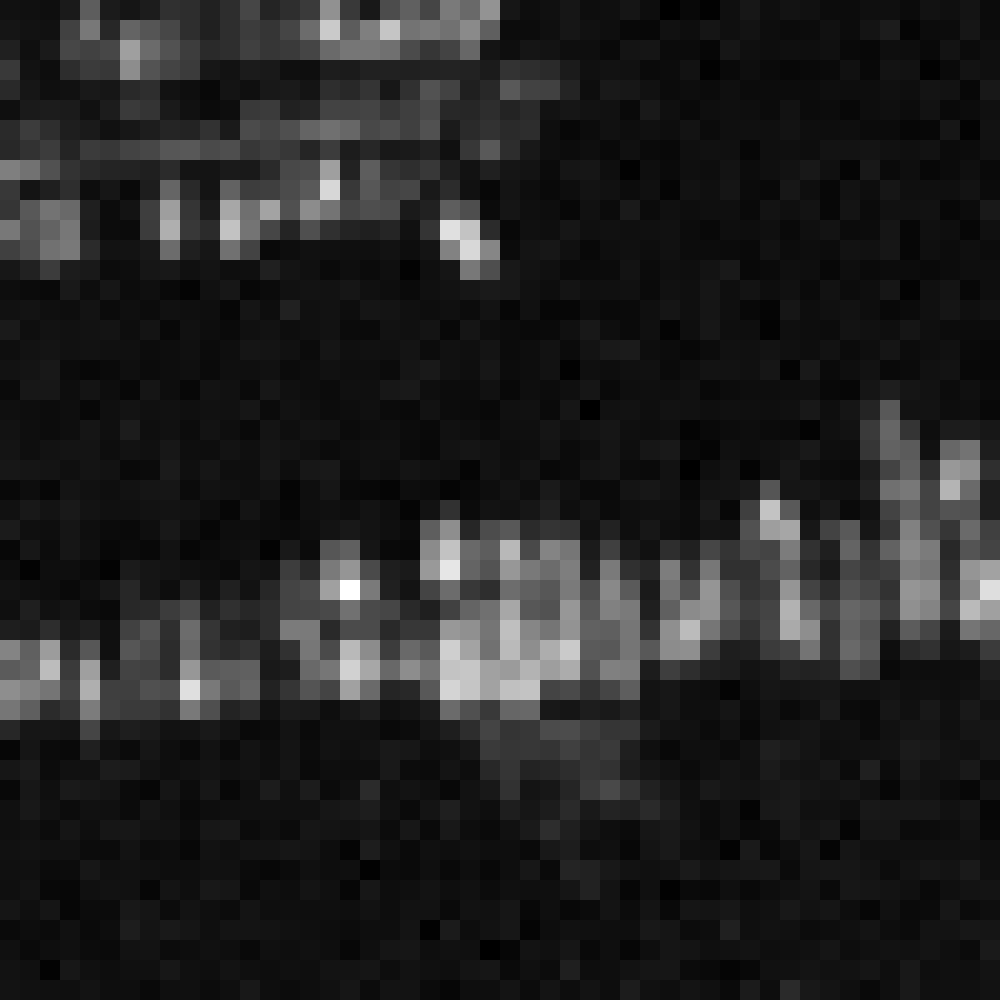
\includegraphics[width=\textwidth]{img/aliasedImg2L2}
\end{subfigure}%
\begin{subfigure}{0.2\textwidth}
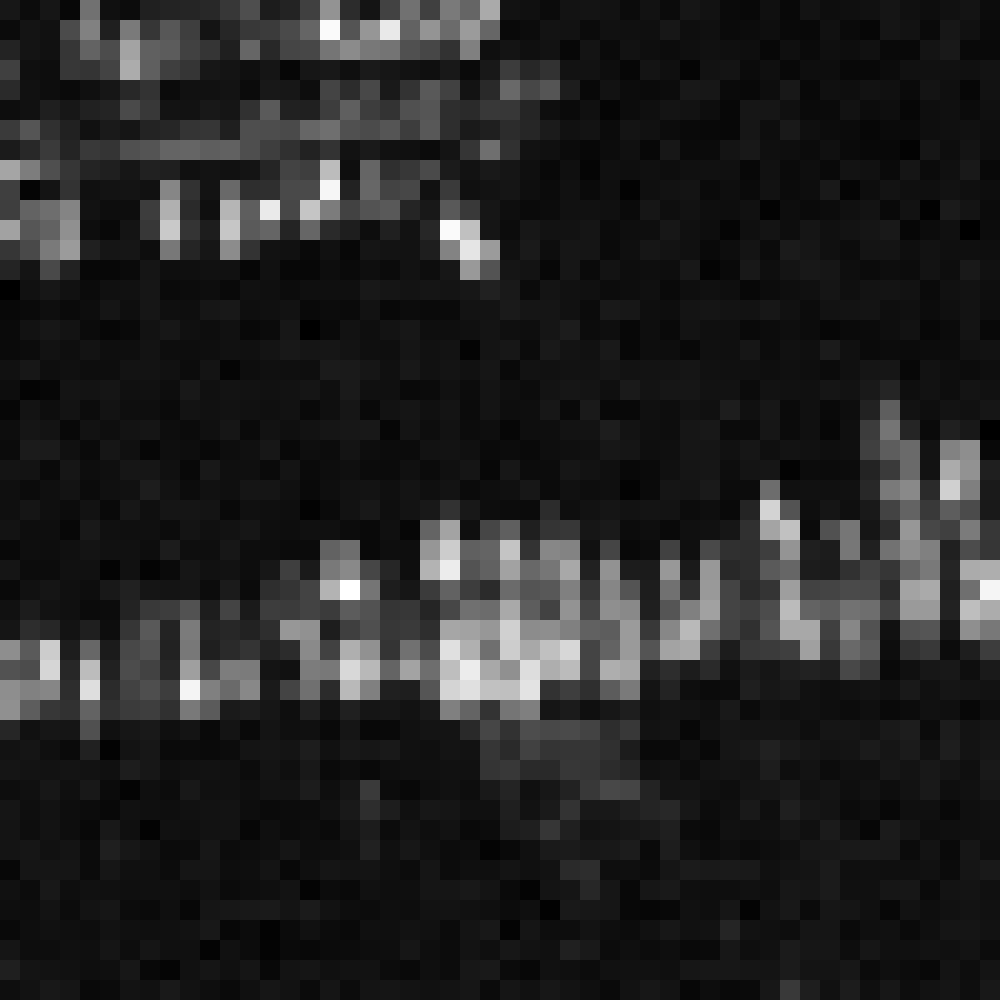
\includegraphics[width=\textwidth]{img/aliasedImg2L3}
\end{subfigure}%
\begin{subfigure}{0.2\textwidth}
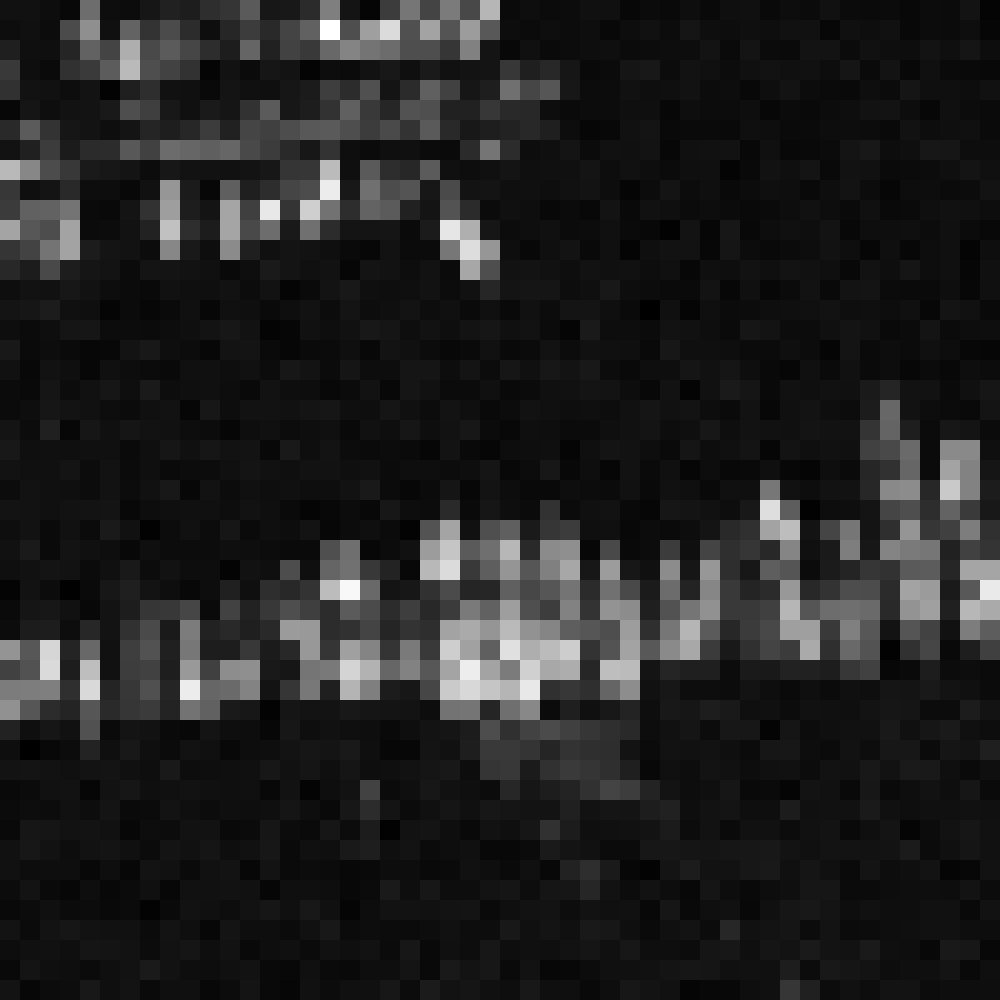
\includegraphics[width=\textwidth]{img/aliasedImg2L4}
\end{subfigure}%
\begin{subfigure}{0.2\textwidth}
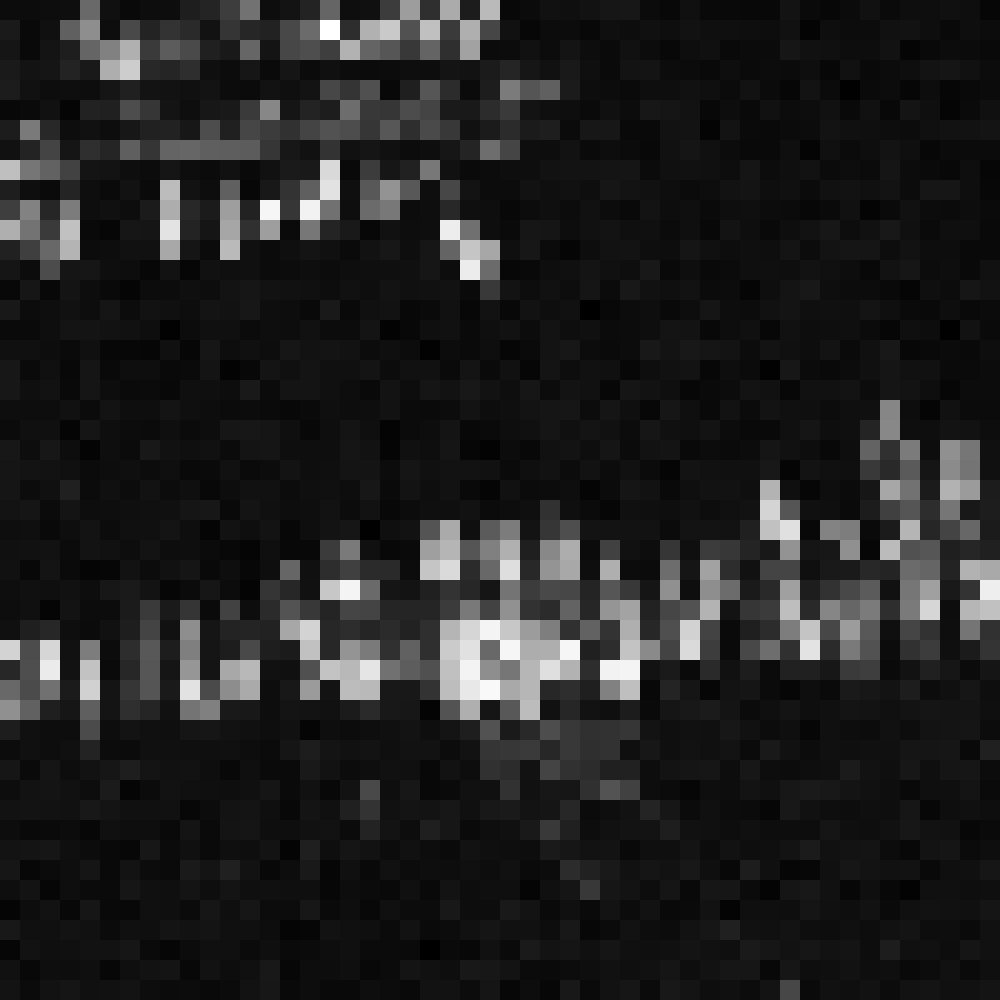
\includegraphics[width=\textwidth]{img/aliasedImg2L5}
\end{subfigure}
\begin{subfigure}{0.2\textwidth}
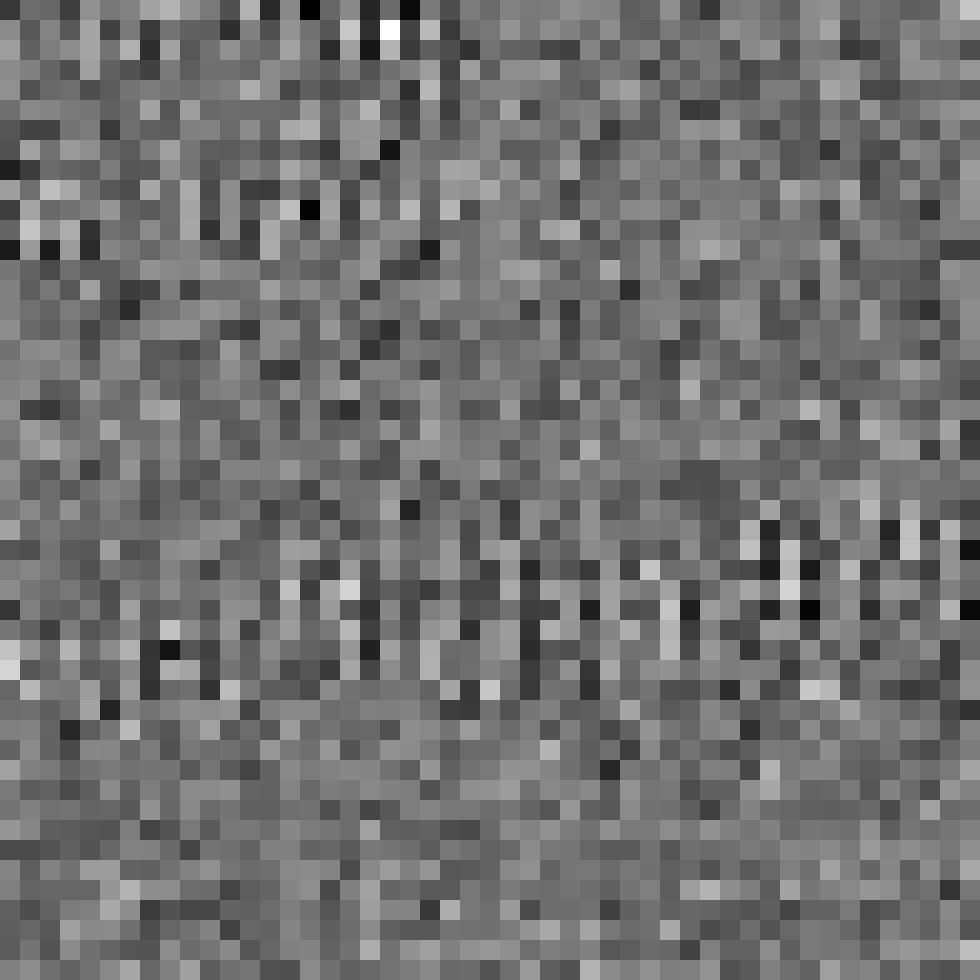
\includegraphics[width=\textwidth]{img/aliasedImgDifL1}
\caption{Level 1}
\end{subfigure}%
\begin{subfigure}{0.2\textwidth}
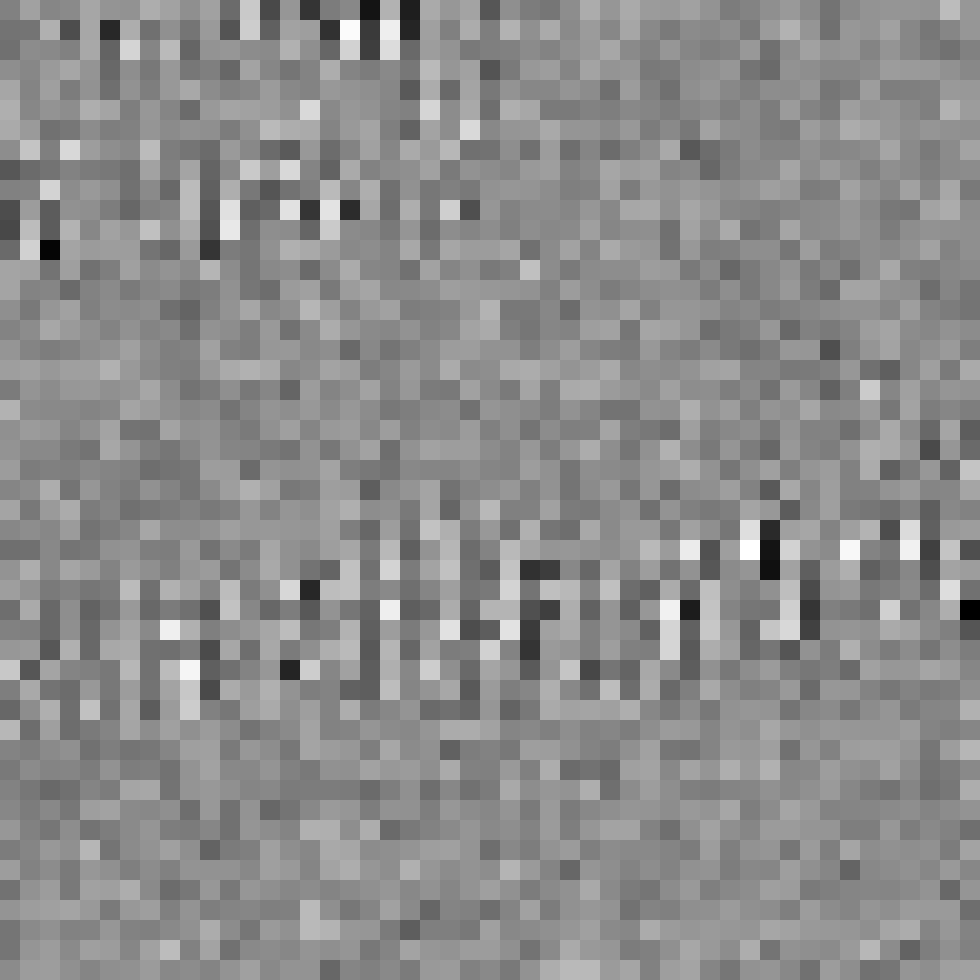
\includegraphics[width=\textwidth]{img/aliasedImgDifL2}
\caption{Level 2}
\end{subfigure}%
\begin{subfigure}{0.2\textwidth}
\includegraphics[width=\textwidth]{img/aliasedImgDifL3}
\caption{Level 3}
\end{subfigure}%
\begin{subfigure}{0.2\textwidth}
\includegraphics[width=\textwidth]{img/aliasedImgDifL4}
\caption{Level 4}
\end{subfigure}%
\begin{subfigure}{0.2\textwidth}
\includegraphics[width=\textwidth]{img/aliasedImgDifL5}
\caption{Level 5}
\end{subfigure}
\caption{Input images shifted by $(-0.25, 0.5)$ used for testing aliasing influence for each aliasing level. \textbf{Top}: $\tilde{I}_1$. \textbf{Center}: $\tilde{I}_2$. \textbf{Bottom}: Difference between compensated images (aliasing + noise effects). Dynamic ranges extended.}
\label{fig:aliasedImages}
\end{figure}

Nevertheless, results in Fig. \ref{fig:aliasingTop10ByLevel} prove that gradient-based methods are still able to deal with aliasing even though they break the brightness constancy constraint on which they are based. To generate this figure, one candidate variant from each evaluated shift estimation algorithm was selected, particularly the variant obtaining the highest average error among all aliasing levels and evaluated shifts. The figure then displays the top ten of these variants. As seen, GBSE approaches using spline interpolation and Gaussian derivatives with $\sigma=0.6$ gave the best results on average using few computational resources. Among the phase correlation methods, the improved gradient correlation approach of \cite{Tzimiropoulos2011} seems the least affected by aliasing, particularly when using short supported filters for gradient calculation (either Gausian with $\sigma=0.3$ or the first order Christmas kernel). The Stone method \cite{Stone_2001} also achieved accurate results without performing apodization of the input images, and should be considered, thanks to its fast implementation (in our computer, among these methods, it turned out to be the fastest). Finally, the Pham bidirectional approach \cite{pham2008} offers a good balance between speed and robustness against aliasing.

\begin{figure}[htpb]
\centering
\includegraphics[width=.75\textwidth]{img/tableAliasingTop10ByLevel}
\caption{Average error by aliasing level of top ten overall methods}
\label{fig:aliasingTop10ByLevel}
\end{figure}

Since aliasing is in general unpredictable and may impact more or less the accuracy depending on the sampling, 
averaging over all shifts may hide interesting cases. Indeed, for most evaluated displacements, the average accuracy of the top 10 approaches never exceed 0.04 pixels of error, however, we observed two situations for which the error was considerably higher. Results for two diferent shifts $(-0.437, 0.5)$ and $(-0.25, 0.5)$ displayed in Fig. \ref{fig:aliasingTop10ByShiftParticular} show a radical change on the methods obtaining the best results. Particularly in those cases, the variants presented by Tzimiropoulos \emph{et al.} \cite{Tzimiropoulos2011} based on gradient correlation obtained the best results, which allows us to conclude that their method is the most robust against aliasing. As for differential methods, the ULS approach again turned out to outperform its class. From these figures two important conclusions should be made. First, that indeed the claims of aliasing robustness of the Christmas derivatives (of first and second order) are true and should be considered when high aliasing exists. And secondly, as expected, that iterative approaches should avoid resampling in the frequency domain, due to a potential increase of artifacts appearing from working with images sampled below the Nyquist rate.

\begin{figure}[htpb]
\begin{subfigure}{0.5\textwidth}
\includegraphics[width=\textwidth]{img/tableAliasingTop10ByShift4}
\end{subfigure}%
\begin{subfigure}{0.5\textwidth}
\includegraphics[width=\textwidth]{img/tableAliasingTop10ByShift8}
\end{subfigure}%
\caption{Average error by aliasing level of top 10 for two particular shifts}
\label{fig:aliasingTop10ByShiftParticular}
\end{figure}
On the other side, an example of the top 10 methods usually resulting for every tested displacement is shown in Fig. \ref{fig:aliasingTop10ByShiftTypical}. GBSE approaches in general proved to be quite robust against low to moderate aliasing scenarios, while also achieving the most accurate results using the fewest computational resources. 

\begin{figure}[htpb]
\centering
\includegraphics[width=.65\textwidth]{img/tableAliasingTop10ByShift13}
\caption{Average error by aliasing level of top 10 methods for a typical shift}
\label{fig:aliasingTop10ByShiftTypical}
\end{figure}

\subsubsection{Conclusions from these experiments}
\label{sec:aliasingConclusionsChapter1}
Three conclusions were drawn from these experiments when dealing with aliasing. First, that GBSE methods (in particular CLS or ULS) offer the best results in terms of accuracy over time consumed. Second, that gradient estimation should be performed using either the kernels proposed by Christmas \cite{christmas1998spatial} or Gaussian derivatives with $\sigma=0.3$ or $\sigma=0.6$. Finally, under extreme aliasing scenarios, the slightly more expensive gradient correlation method proved to offer the best results.


\subsection{Computational cost comparison}
\label{sec:ComputationalCostChapter1}
To provide an idea of the computational resources required for each method, we averaged execution times for 1000 executions using several shift magnitudes and noises. The processing time of each method was measured using non-optimized Matlab implementations on an Intel Xeon E5-2650 CPU. Results, shown in Fig.~\ref{fig:avgTimes}, are orientative and should not be taken as a definitive measurement. Indeed, some displayed times are evidently not representative. As an example, the subspace method of Robinson (SS-ROBINSON-Wtw) should reflect lower processing time given its low complexity. Both Sinc fitting (PC-SINC-Wtw) together with gradient correlation methods based on non-linear kernel fitting (GC11) employ considerable time due to the optimization performed. The optimization is done by means of the $lsqcurvefit$ function in Matlab which besides the optimization procedure, also does an important amount of overhead work used to initialize internal components that would not exist if a more direct implementation were available.

\begin{figure}[ht!]
	\centering
	\includegraphics[width=.8\textwidth]{img/avgTimes}
	\caption{Average execution time for some representative methods}
	\label{fig:avgTimes}
\end{figure}

To contrast processing time with precision, we averaged the errors for each method over all noise levels and over the first three categories of shift magnitudes. We also made this comparison for each shift magnitude individually. Results displayed in Fig.~\ref{fig:avgTimesVsAccuracy} and Fig.~\ref{fig:avgTimesVsAccuracyByShift} represent a general summary of this review. 

\begin{figure}[ht!]
	\centering
	\includegraphics[width=1\textwidth]{img/avgTimesVsAccuracy}
	\caption{Average execution time (log scale) vs accuracy for some representative methods averaged over the first three shift magnitudes and all noise levels}
	\label{fig:avgTimesVsAccuracy}
\end{figure}

\begin{figure}[ht!]
	\centering
	\begin{subfigure}{.5\linewidth}
		\includegraphics[width=1\textwidth]{img/avgTimesVsAccuracyShift1}
		\caption{\footnotesize{Shift magnitude category 1}}
	\end{subfigure}%
	\begin{subfigure}{.5\linewidth}
		\includegraphics[width=1\textwidth]{img/avgTimesVsAccuracyShift2}
		\caption{\footnotesize{Shift magnitude category 2}}
	\end{subfigure}
	\begin{subfigure}{.5\linewidth}
	\vspace{3mm}
		\includegraphics[width=1\textwidth]{img/avgTimesVsAccuracyShift3}
		\caption{\footnotesize{Shift magnitude category 3}}
	\end{subfigure}%
	\begin{subfigure}{.5\linewidth}
	\vspace{3mm}
		\includegraphics[width=1\textwidth]{img/avgTimesVsAccuracyShift4}
		\caption{\footnotesize{Shift magnitude category 4}}
	\end{subfigure}%
		
	\caption{Average execution time (log scale) vs accuracy for some representative methods for each shift magnitude category averaged over all noise levels}
	\label{fig:avgTimesVsAccuracyByShift}
\end{figure}

Based on the provided figures, we conclude that gradient-based methods not only achieve more accurate results but also require fewer computational resources. When the shift estimation must cope with severe computational constraints, single iterated GBSE approaches are recommended, and the best option, as seen before, depends on the shift size. If the underlying shift magnitudes are small, LS or TLS methods using short gradient estimation kernels support should be selected. If shifts are uniformly distributed along the [-1,1] interval, the bidirectional bias corrected (ULS) approach proves to be the best choice. For larger displacements, the recommended approach is  multiscale GBSE, the method of Hoge \cite{Hoge_2003} or the approach of Stone \cite{Stone_2001}. Under less demanding time constraints, gradient-correlation-based methods should be considered.

\subsection{Evaluation on real MRI images}
\label{sec:realMRIChapter1}
We evaluated every method against a set of real MRI images of a grapefruit. This set, provided by Hoge \cite{Hoge_2003} together with its ground truth, is used in several articles of the state-of-the-art to contrast existing approaches. It consists of five different images shifted. To offer a more complete evaluation, we tested all shift estimation methods under  five different noise levels injected to the images. Again, we assumed additive white Gaussian noise and the standard deviation for each noise level is shown in Table \ref{tab:noiseLevels}. In Fig.~\ref{fig:grapefruitMRI} we show the original image along with two other versions generated by manually adding white Gaussian noise. 
\begin{figure}[htpb]
\begin{subfigure}{0.33\textwidth}
	\includegraphics[width=1\textwidth]{img/grapeMRILevel1}
\end{subfigure}%
\begin{subfigure}{0.33\textwidth}
	\includegraphics[width=1\textwidth]{img/grapeMRILevel3}
\end{subfigure}%
\begin{subfigure}{0.33\textwidth}
	\includegraphics[width=1\textwidth]{img/grapeMRILevel5}
\end{subfigure}%
\caption{First image of the MRI set provided by Hoge \cite{Hoge_2003} under different noise levels. \textbf{Left}: Original image (level 1). \textbf{Middle}: $\sigma=0.015$ (level 3). \textbf{Right}: $\sigma=0.055$ (level 5)}
\label{fig:grapefruitMRI}	
\end{figure}

For this experiment and due to the length of the underlying shifts to estimate, we included two multiscale GBSE methods using four and five scales, with increasing iterations across scales, spline interpolation and hypomode gradient, denoted MS-4 and MS-5 respectively. Results in Table \ref{tab:grapefruitMRIResults} show that errors were considerably higher than what was obtained in the previous simulated experiments. To explain this, we used the ground truth to resample each image with respect to the other. In Fig.~\ref{fig:grapefruitMRIDiff} we observe the absolute difference between an image and another aligned with it using the ground truth. As can be noted, for both left and middle images, the difference is considerably high on the image edges, which proves the images are not correctly registered, even though the ground truth was used. For the third case, the images are better registered and what is observed is mainly (signal dependent) noise  and some minor aliasing. Therefore, this explains the significative errors achieved by most methods. This fact is indeed of major importance, since several articles compared their methods using this dataset \cite{Hoge_2003, Ren_2010, Ren_2014, Tzimiropoulos2011}. Based on this result, the analysis of performance for every method for the whole dataset is not feasible, thus ommited. However, as an example, we evaluated every method by estimating the shift between the fourth and the fifth images of the dataset, for which the provided ground truth appeared to be faithful (by observing the difference between both aligned images). Results appearing in Table \ref{tab:grapefruitMRIResultsCorrect} again prove that the multiscale GBSE approach is the best overall option, however, by a shorter margin in this case. The next best competitor is again gradient-correlation-based methods \cite{Tzimiropoulos2011, Argyriou2004}. The iterative periodic correlation method \cite{Sidick2011} also gathered acceptable results, however the obtained error was too high for the lowest evaluated SNR. As for phase-correlation approaches, the esinc \cite{Argyriou2006} almost always appear as the best option for this images. The top 10 methods computed by taking the averages over all noise levels for these two images is shown in Table \ref{tab:grapefruitMRIResultsCorrectAverages}. We observe that only six method types achieved acceptable results for all noise levels.
%, although we observe that as the noise increases, both gradient correlation and GBSE methods appear in the top ten list, which reflects our previous findings. Nevertheless, it should be noted that this could be coincidental.

\begin{table}[htpb]
\scriptsize
\setlength{\tabcolsep}{1pt}
\centering
\begin{tabular}{c|c|c|c|c}
$\sigma = 0.000$ & $\sigma = 0.005$ & $\sigma = 0.015$ & $\sigma = 0.025$ & $\sigma = 0.055$\\ \hline 
\begin{tabular}{l}
0.1753 SS-HOGE-Wbh\\ 
0.1815 PC-LCM-1D2\\ 
0.1850 APC-0.0001\\ 
0.1894 NGC04-Gg0.6\\ 
0.1942 NGC11-G5\\ 
0.1942 GC11-G5\\ 
0.1962 MS-4,4321-IsssssGch3\\ 
0.2025 GC04-G6\\ 
0.2043 SDF-2QI\\ 
0.2045 CFI-2QI\\  
\end{tabular} & 
\begin{tabular}{l}
0.1742 PC-LCM-2D2\\ 
0.1856 SS-HOGE-Wbh\\ 
0.1908 APC-0.0001\\ 
0.1935 NGC11-G6\\ 
0.1938 GC11-G6\\ 
0.1948 MS-4\\ 
0.2005 GC04-Gg1\\ 
0.2046 CFI-2QI\\ 
0.2046 SDF-2QI\\ 
0.2115 ADF2-2QI\\ 
\end{tabular} & 
\begin{tabular}{l}
0.1913 NGC11-Gch3\\ 
0.1927 PC-LCM-2D1\\ 
0.1941 APC-0.0001\\ 
0.1953 GC11-Gch3\\ 
0.1985 GC04-G6\\ 
0.2039 GBSE-MS-5\\ 
0.2065 SDF-2QI\\ 
0.2068 CFI-2QI\\ 
0.2155 ADF2-2QI\\ 
0.2160 ADF-2QI\\  
\end{tabular} & 
\begin{tabular}{l}
0.2021 GBSE-MS-4\\ 
0.2075 APC-0.0001\\ 
0.2119 NGC11-G6\\ 
0.2121 GC11-G6\\ 
0.2142 GC04-Gg1\\ 
0.2161 PC-ESINC-Wbh\\ 
0.2270 SDF-2QI\\ 
0.2279 CFI-2QI\\ 
0.2304 ADF2-2QI\\ 
0.2307 ADF-2QI\\  
\end{tabular} & 
\begin{tabular}{l}
0.2132 GBSE-MS-5\\ 
0.2137 NGC11-Gg0.6\\ 
0.2210 GC11-Gg0.6\\ 
0.2241 GC04-Gg1\\ 
0.2403 ADF-2QI\\ 
0.2403 ADF2-2QI\\ 
0.2461 CFI-2QI\\ 
0.2472 SDF-2QI\\ 
0.2493 PC-GUIZAR-10\\ 
0.2549 APC-0.0001\\ 
\end{tabular}
\end{tabular}
\caption{Error values for top 10 best variants of each method averaged over all measurements for the grapefruit MRI dataset by injecting different amounts of additive white Gaussian noise. Note that these results cannot be relied upon, as the ground truth provided for this dataset appears to be incorrect.}
\label{tab:grapefruitMRIResults}
\end{table}

\begin{figure}[htpb]
\begin{subfigure}{0.33\textwidth}
	\includegraphics[width=1\textwidth]{img/grapeMRIDif1with3.png}
\end{subfigure}%
\begin{subfigure}{0.33\textwidth}
	\includegraphics[width=1\textwidth]{img/grapeMRIDif1with5.png}
\end{subfigure}%
\begin{subfigure}{0.33\textwidth}
	\includegraphics[width=1\textwidth]{img/grapeMRIDif3with5.png}
\end{subfigure}%
\caption{Absolute value of the difference between aligned images based on the ground truth information provided by Hoge \cite{Hoge_2003} using the original images. \textbf{Left}: Between the first and the third image. \textbf{Middle}: Between the first and the fifth image. \textbf{Right}: Between the third and the fifth image. Dynamic ranges extended for improved visual perception.}
\label{fig:grapefruitMRIDiff}	
\end{figure}

\begin{table}[htpb]
\scriptsize
\setlength{\tabcolsep}{1pt}
\hspace{-5mm}
\begin{tabular}{c|c|c|c|c}
$\sigma = 0.000$ & $\sigma = 0.005$ & $\sigma = 0.015$ & $\sigma = 0.025$ & $\sigma = 0.055$\\ \hline 
\begin{tabular}{l}
0.0024 MS-3,321-IfssGg1\\ 
0.0056 PC-ESINC-Wex\\ 
0.0062 NGC04-Gg1\\ 
0.0095 SS-HOGE-Wtw\\ 
0.0115 NGC11-Gg1\\ 
0.0118 APC-0.0001\\ 
0.0127 GC11-Gch3\\ 
0.0243 GC04-Gg1\\ 
0.0842 ACC-0.0001\\ 
0.1370 PCFOO\\ 
\end{tabular} & 
\begin{tabular}{l}
0.0136 MS-3,321-IsssGsim3\\ 
0.0162 GC11-Gch1\\ 
0.0167 PC-GUIZAR-10\\ 
0.0175 NGC11-Gch2\\ 
0.0199 APC-3It\\ 
0.0245 GC04-Gg1\\ 
0.0269 SS-HOGE-Wtw\\ 
0.2594 PCFOO\\ 
0.3413 ACC-3It\\ 
3.5684 CLS-4-IdGfa7\\ 
\end{tabular} & 
\begin{tabular}{l}
0.0229 MS-3,321-IsssGsim5\\ 
0.0264 GC11-Gg0.3\\ 
0.0275 NGC11-Gch1\\ 
0.0307 GC04-Gg1\\ 
0.0394 APC-2It\\ 
0.0423 PC-ESINC-Wtw\\ 
0.1838 SS-HOGE-Whw\\ 
0.2930 PCFOO\\ 
0.4506 ACC-3It\\ 
4.2313 CLS-4-IfGfa7\\ 
\end{tabular} & 
\begin{tabular}{l}
0.0296 MS-3,321-IsssGfa3\\ 
0.0357 GC11-Gg0.6\\ 
0.0377 NGC11-Gg0.6\\ 
0.0420 GC04-Gg1\\ 
0.0625 APC-0.01\\ 
0.0690 PC-ESINC-Wtw\\ 
0.3425 PCFOO\\ 
0.3645 SS-REN2014-Wtw\\ 
0.7081 ACC-2It\\ 
4.2080 LS-4-IdGfa7\\ 
\end{tabular} & 
\begin{tabular}{l}
0.0587 MS-3,321-IdssGfa5\\ 
0.0597 GC11-Gg1\\ 
0.0634 NGC11-Gg1\\ 
0.0672 GC04-Gg1\\ 
0.1260 PC-ESINC-Wtw\\ 
0.1458 APC-2It\\ 
0.4030 PCFOO\\ 
0.9873 ACC-2It\\ 
1.5331 SS-REN2014-Whw\\ 
4.7611 LS-4-IsGfa7\\ 
\end{tabular}
\end{tabular}
\caption{Average error values for top 10 best variants of each method by estimating the shift between the fourth and the fifth images of the grapefruit MRI dataset (ground truth shift: $(7.68,0)$) by injecting different amounts of additive white Gaussian noise.}
\label{tab:grapefruitMRIResultsCorrect}
\end{table}

\begin{table}[htpb]
\scriptsize
\setlength{\tabcolsep}{.5pt}
\centering
\begin{tabular}{|c|}
Avg \\ \hline
\begin{tabular}{l}
0.0282 MS-4,4321-IsssssGsim3 \\
0.0317 GC11-Gg0.6 \\
0.0332 NGC11-Gg0.6 \\
0.0377 GC04-Gg1 \\
0.0558 PC-ESINC-Wtw \\
0.0563 APC-3It \\
0.2870 PCFOO \\
0.5266 ACC-3It \\
0.5683 SS-REN2014-Whw \\
4.0268 CLS-4-IdGfa7 \\ \hline
\end{tabular}
\end{tabular}
\caption{Average error values for all levels of noise for top 10 best variants of each method by estimating the shift between the fourth and the fifth images of the grapefruit MRI dataset (ground truth shift: $(7.68,0)$).}
\label{tab:grapefruitMRIResultsCorrectAverages}
\end{table}


\section{Concluding Remarks}
\label{sec:conclusionsChapter1}

In this article we performed an in-depth review of fast and accurate shift estimation methods.  Although most recent work on shift estimation is based on phase-correlation methods, GBSE approaches proved to be more accurate, stable and run faster than phase correlation approaches, although they are limited to subpixel estimation or required to be used in a pyramidal multiscale approach in order to estimate larger shifts. On the other side, gradient-correlation-based methods showed an improvement over phase correlation methods, particularly under higher noise or highly aliased scenarios, although they usually require more computational resources. Throughout this article, we found out that if \emph{a-priori} knowledge is available regarding the maximum shift magnitude to estimate, then better estimation accuracies can be achieved by selecting a more suitable variant for each method. We provided the reader with such fine-tuning tips. Another interesting discovery is that one of the most used ground truth data used for comparison among state-of-the-art methods is not precise and should be avoided. Finally and most importantly, based on this study and on the characteristics of the underlying shift estimation problem, a practical recipe is offered to the community in order to achieve fast and accurate shift estimation.


Despite the extensive length of this review, we plan to include other useful information. First, some interesting methods were excluded from the final comparison due to the complexity of their implementations or high computational times. These were the methods of Takita \cite{Takita2003}, Balci \cite{Balci_2005}, Leprince \cite{leprince2007automatic} and the recent method of Tong \emph{et al.} \cite{tong2015novel}. We plan to add them in the future. Another considered task, is to test the robustness of each method under varying illumination conditions between the images. We believe that in these cases, if no histogram equalization is possible, GBSE methods should be avoided and phase or gradient correlation approaches would become first options. Also, we plan on combining different presented approaches to obtain a more general method yielding good results on every situation. Finally, we plan to provide publicly a ground truth dataset to be used for comparison of shift estimation methods, considering all difficulties usually faced on such task.

\section*{Acknowledgements}
	I would like to thank Prof. Vasileios Argyriou for providing several source codes helping the development of this review. We also thank Dr. Tuan Q. Pham for fruitful comments and discussions.

